\documentclass[8pt,twocolumn,letterpaper]{extarticle}
\usepackage[top=14.5mm,bottom=14mm,left=12mm,right=12mm,headheight=10pt,headsep=4.5mm,footskip=6.5mm,columnsep=4.8mm]{geometry}
\usepackage{amsmath,amssymb,amsfonts,bm,mathtools}
\usepackage{graphicx}
\usepackage{booktabs}
\usepackage{xcolor}
\usepackage{fancyhdr}
\usepackage{titlesec}
\usepackage{caption}
\usepackage{enumitem}
\usepackage{microtype}
\usepackage{newtxtext,newtxmath}
\usepackage{flushend}
\usepackage{xurl}
\usepackage[colorlinks=true,linkcolor=navyblue,citecolor=navyblue,urlcolor=navyblue]{hyperref}

\definecolor{navyblue}{HTML}{002F6C}
\definecolor{crimson}{HTML}{C53030}
\definecolor{darkgray}{HTML}{4A5568}
\definecolor{charcoal}{HTML}{1A202C}
\definecolor{abstractbg}{HTML}{F8FAFC}

\DeclareMathOperator{\logm}{logm}
\DeclareMathOperator{\Tr}{Tr}
\DeclareMathOperator{\diag}{diag}

\pagestyle{fancy}
\fancyhf{}
\renewcommand{\headrulewidth}{0pt}
\fancyhead[L]{\sffamily\bfseries\fontsize{7.5pt}{9pt}\selectfont\textcolor{darkgray}{Singh \& Singh}}
\fancyhead[R]{\sffamily\bfseries\fontsize{7.5pt}{9pt}\selectfont\textcolor{darkgray}{Journal of Chemical Theory and Computation}}
\fancyfoot[L]{\sffamily\fontsize{7pt}{8.5pt}\selectfont\textcolor{darkgray}{Scalable Contact-Gated Stochastic Operators for Macromolecular Dynamics}}
\fancyfoot[R]{\sffamily\bfseries\fontsize{8pt}{9.5pt}\selectfont\textcolor{charcoal}{\thepage}}

\titleformat{\section}{\sffamily\bfseries\fontsize{8.5pt}{10pt}\selectfont\color{navyblue}}{}{0pt}{}
\titlespacing*{\section}{0pt}{5pt}{2pt}

\titleformat{\subsection}{\sffamily\bfseries\itshape\fontsize{7.7pt}{9.2pt}\selectfont\color{charcoal}}{}{0pt}{}
\titlespacing*{\subsection}{0pt}{4pt}{1.5pt}

\captionsetup{font={scriptsize}, labelfont={bf,sf,color=navyblue}, labelsep=period, justification=justified, singlelinecheck=false}

\setlength{\parindent}{9pt}
\setlength{\parskip}{0.75pt}
\setlength{\abovedisplayskip}{2.5pt}
\setlength{\belowdisplayskip}{2.5pt}
\setcounter{dbltopnumber}{3}
\renewcommand{\dbltopfraction}{0.88}
\renewcommand{\textfraction}{0.08}
\emergencystretch=1.8em

% Auto-generated verified empirical metrics (zero hardcoded empirical numbers)
% Auto-generated by version4_godtier/analysis/r41_master_synthesis.py
% ZERO HARDCODING: Every value is extracted directly from SHA-256-verified JSON results.
\newcommand{\vFourTotalSystems}{15}
\newcommand{\vFourNumProteins}{13}
\newcommand{\vFourNumExplicitPmeSystems}{6}
\newcommand{\vFourMinDim}{2}
\newcommand{\vFourMinProteinDim}{18}
\newcommand{\vFourMaxProteinDim}{738}
\newcommand{\vFourTotalAtlasFrames}{890,000}
\newcommand{\vFourTotalSamplingNs}{890}
\newcommand{\vFourTotalSamplingUs}{0.89}
\newcommand{\vFourRepSpectralMeanRTwo}{0.996}
\newcommand{\vFourExplicitParticlesLysozyme}{17,110}
\newcommand{\vFourExplicitParticlesDhfr}{20,837}
\newcommand{\vFourExplicitParticlesAdk}{40,110}
\newcommand{\vFourExplicitParticlesMbp}{49,215}
\newcommand{\vFourMaxExplicitAtomsMbp}{49,215}
\newcommand{\vFourRankAlpha}{0.874}
\newcommand{\vFourRankExponent}{0.874}
\newcommand{\vFourRankPrecoeff}{0.735}
\newcommand{\vFourRankPrefactor}{0.735}
\newcommand{\vFourRankRTwo}{0.969}
\newcommand{\vFourRankExpCILow}{0.795}
\newcommand{\vFourRankExpCIHigh}{1.106}
\newcommand{\vFourRankDeltaAICc}{-4.8}
\newcommand{\vFourRankContAlpha}{0.919}
\newcommand{\vFourRankContPrefactor}{0.577}
\newcommand{\vFourRankContRTwo}{0.978}
\newcommand{\vFourProteinsOnlyAlpha}{1.059}
\newcommand{\vFourProteinsOnlyPrefactor}{0.283}
\newcommand{\vFourProteinsOnlyRTwo}{0.978}
\newcommand{\vFourPRAlpha}{0.494}
\newcommand{\vFourPRExponent}{0.494}
\newcommand{\vFourPRPrecoeff}{1.061}
\newcommand{\vFourPRPrefactor}{1.061}
\newcommand{\vFourPRRTwo}{0.741}
\newcommand{\vFourPRExpCILow}{0.332}
\newcommand{\vFourPRExpCIHigh}{0.666}
\newcommand{\vFourPRDeltaAICc}{-18.15}
\newcommand{\vFourDiffOpRankPrefactor}{0.799}
\newcommand{\vFourDiffOpRankAlpha}{0.930}
\newcommand{\vFourDiffOpRankCILow}{0.904}
\newcommand{\vFourDiffOpRankCIHigh}{0.998}
\newcommand{\vFourDiffOpRankRTwo}{0.997}
\newcommand{\vFourDiffOpDeltaAICc}{-14.39}
\newcommand{\vFourProteinsOnlyNullCZero}{0.376}
\newcommand{\vFourProteinsOnlyNullRTwo}{0.975}
\newcommand{\vFourNullRankExponent}{0.961}
\newcommand{\vFourRankTrainPrefactor}{0.762}
\newcommand{\vFourRankTrainExponent}{0.819}
\newcommand{\vFourRankTrainLinearCZero}{0.402}
\newcommand{\vFourRankExtrapolationMAPE}{35.7}
\newcommand{\vFourRankLinearNullExtrapolationMAPE}{10.0}
\newcommand{\vFourMaxCompressionRatioMbp}{2.37}
\newcommand{\vFourNullVsActualRatioMbp}{1.62}
\newcommand{\vFourMeanPeptideCrankshaftR}{-0.603}
\newcommand{\vFourStdPeptideCrankshaftR}{0.054}
\newcommand{\vFourMeanIntraResR}{-0.211}
\newcommand{\vFourKeffMean}{5.97}
\newcommand{\vFourMinProteinSparsityPct}{71.2}
\newcommand{\vFourMaxProteinSparsityPct}{99.3}
\newcommand{\vFourKeffMin}{4.70}
\newcommand{\vFourKeffMax}{7.95}
\newcommand{\vFourSparsityPctMbp}{99.3}
\newcommand{\vFourContactEnrichMin}{1.07}
\newcommand{\vFourContactEnrichMax}{3.05}
\newcommand{\vFourContactEnrichMean}{2.17}
\newcommand{\vFourChigBeta}{2.205}
\newcommand{\vFourChigDeltaAICc}{-1.85}
\newcommand{\vFourChigCrankshaftParity}{-0.512}
\newcommand{\vFourChigSparsityPct}{71.2}
\newcommand{\vFourMemExpDense}{2.00}
\newcommand{\vFourMemExpContact}{1.06}
\newcommand{\vFourTimeExpGlasso}{1.27}
\newcommand{\vFourTimeExpChordal}{1.13}
\newcommand{\vFourMemCompressionMbp}{65.8}
\newcommand{\vFourSpeedupMbpVsGlasso}{77.3}
\newcommand{\vFourSpeedupMbpVsDense}{10.3}
\newcommand{\vFourTimeMsContactMbp}{26.7}
\newcommand{\vFourTimeMsDenseMbp}{275.4}
\newcommand{\vFourTimeMsGlassoMbp}{2062.7}
\newcommand{\vFourMemKbContactMbp}{64.7}
\newcommand{\vFourMemKbDenseMbp}{4255.0}
\newcommand{\vFourLogLikPerDMbpContact}{+0.303}
\newcommand{\vFourLogLikPerDMbpDense}{+0.205}
\newcommand{\vFourLogLikPerDMbpGlasso}{+0.247}
\newcommand{\vFourMbpContactFrob}{0.501}
\newcommand{\vFourMbpDenseFrob}{0.601}
\newcommand{\vFourLawFourWinner}{linear Einstein equipartition}
\newcommand{\vFourChigCoreMAPE}{12.33}
\newcommand{\vFourChigPowerMAPE}{12.79}
\newcommand{\vFourSASALawHeldOutMAPE}{12.33}
\newcommand{\vFourAlphaBuriedCore}{1.00}
\newcommand{\vFourAlphaSurfaceLoop}{1.28}
\newcommand{\vFourAlphaShortPeptide}{1.57}
\newcommand{\vFourGammaIntExposedSurface}{14.0}
\newcommand{\vFourNMRCrankSpearman}{+0.255}
\newcommand{\vFourNMRCrankPearson}{+0.522}
\newcommand{\vFourNMRCrankPValue}{3.50e-07}
\newcommand{\vFourNMRCrankRMSE}{0.138}
\newcommand{\vFourNMRPooledSpearman}{+0.146}
\newcommand{\vFourNMRPooledRMSE}{0.099}
\newcommand{\vFourNMRIntraSpearman}{+0.286}
\newcommand{\vFourNMRIntraPearson}{+0.500}
\newcommand{\vFourGNMPooledSpearman}{+0.378}
\newcommand{\vFourGNMPooledPearson}{+0.494}
\newcommand{\vFourDirectMDPooledSpearman}{+0.311}
\newcommand{\vFourNMRMeanProteinSpearmanCrank}{+0.483}
\newcommand{\vFourNMRMeanProteinSpearmanFlank}{+0.462}
\newcommand{\vFourNMRMeanProteinSpearmanGNM}{+0.408}
\newcommand{\vFourNMRSpearmanUbq}{+0.512}
\newcommand{\vFourNMRPearsonUbq}{+0.921}
\newcommand{\vFourNMRRMSEUbq}{0.110}
\newcommand{\vFourNMRFlankSpearmanUbq}{+0.447}
\newcommand{\vFourNMRIntraSpearmanUbq}{+0.499}
\newcommand{\vFourNMRGnmSpearmanUbq}{+0.505}
\newcommand{\vFourNMRDirectMDSpearmanUbq}{+0.487}
\newcommand{\vFourNMRSpearmanGbOne}{+0.746}
\newcommand{\vFourNMRPearsonGbOne}{+0.601}
\newcommand{\vFourNMRRMSEGbOne}{0.153}
\newcommand{\vFourNMRFlankSpearmanGbOne}{+0.732}
\newcommand{\vFourNMRIntraSpearmanGbOne}{+0.806}
\newcommand{\vFourNMRGnmSpearmanGbOne}{+0.384}
\newcommand{\vFourNMRDirectMDSpearmanGbOne}{+0.740}
\newcommand{\vFourNMRSpearmanLysozyme}{+0.491}
\newcommand{\vFourNMRPearsonLysozyme}{+0.494}
\newcommand{\vFourNMRRMSELysozyme}{0.137}
\newcommand{\vFourNMRFlankSpearmanLysozyme}{+0.473}
\newcommand{\vFourNMRIntraSpearmanLysozyme}{+0.517}
\newcommand{\vFourNMRGnmSpearmanLysozyme}{+0.391}
\newcommand{\vFourNMRDirectMDSpearmanLysozyme}{+0.520}
\newcommand{\vFourNMRSpearmanDhfr}{+0.182}
\newcommand{\vFourNMRPearsonDhfr}{+0.190}
\newcommand{\vFourNMRRMSEDhfr}{0.146}
\newcommand{\vFourNMRFlankSpearmanDhfr}{+0.199}
\newcommand{\vFourNMRIntraSpearmanDhfr}{+0.200}
\newcommand{\vFourNMRGnmSpearmanDhfr}{+0.354}
\newcommand{\vFourNMRDirectMDSpearmanDhfr}{+0.257}
\newcommand{\vFourBFactorMeanSpearman}{+0.276}
\newcommand{\vFourBFactorCount}{8}
\newcommand{\vFourBFactorSpearmanUbiquitin}{+0.221}
\newcommand{\vFourBFactorSpearmanGbOne}{+0.221}
\newcommand{\vFourBFactorSpearmanLysozyme}{+0.467}
\newcommand{\vFourBFactorSpearmanDhfr}{+0.240}
\newcommand{\vFourBFactorSpearmanBpti}{+0.346}
\newcommand{\vFourBFactorSpearmanBarnase}{+0.322}
\newcommand{\vFourBFactorSpearmanAdk}{+0.206}
\newcommand{\vFourBFactorSpearmanMbp}{+0.188}
\newcommand{\vFourLOPOMeanRTwo}{+0.359}
\newcommand{\vFourLOPOMeanSpearman}{+0.706}
\newcommand{\vFourLOPOMeanPearson}{+0.735}
\newcommand{\vFourLOPOMeanFrobErrPct}{45.5}
\newcommand{\vFourLOPOGbdtRTwo}{+0.410}
\newcommand{\vFourLOPOGbdtSpearman}{+0.721}
\newcommand{\vFourLOPOGbdtFrobErrPct}{44.8}
\newcommand{\vFourLOPORidgeNineRTwo}{+0.350}
\newcommand{\vFourLOPORidgeNineSpearman}{+0.698}
\newcommand{\vFourLOPOConstFrobErrPct}{60.0}
\newcommand{\vFourLOPONoiseFloorFrobPct}{16.9}
\newcommand{\vFourInteriorMobilityMean}{0.0419}
\newcommand{\vFourInteriorMobilityCVPct}{24.7}
\newcommand{\vFourHelixMobilityMean}{0.0320}
\newcommand{\vFourStrandMobilityMean}{0.0407}
\newcommand{\vFourCoilMobilityMean}{0.0485}
\newcommand{\vFourAdkHingeAUROC}{0.644}
\newcommand{\vFourAdkHingePRAUC}{0.348}
\newcommand{\vFourAdkApoMdToroidalAUROC}{0.630}
\newcommand{\vFourAdkApoMdToroidalSpearman}{+0.312}
\newcommand{\vFourAdkANMAUROC}{0.647}
\newcommand{\vFourAdkANMPRAUC}{0.230}
\newcommand{\vFourAdkApoMdCartAUROC}{0.580}
\newcommand{\vFourAdkDynDomAUROC}{0.400}
\newcommand{\vFourAdkDynDomApoToroidalAUROC}{0.529}
\newcommand{\vFourAdkPrecAtFifteen}{0.400}
\newcommand{\vFourAdkANMPrecAtFifteen}{0.267}
\newcommand{\vFourAdkDynDomApoPrecAtFifteen}{0.267}
\newcommand{\vFourAdkDynDomANMPrecAtFifteen}{0.000}
\newcommand{\vFourMbpHingeAUROC}{0.421}
\newcommand{\vFourMbpApoMdToroidalAUROC}{0.690}
\newcommand{\vFourMbpApoMdToroidalSpearman}{+0.315}
\newcommand{\vFourMbpANMAUROC}{0.446}
\newcommand{\vFourMbpApoMdCartAUROC}{0.635}
\newcommand{\vFourMbpDynDomAUROC}{0.619}
\newcommand{\vFourMbpDynDomApoToroidalAUROC}{0.693}
\newcommand{\vFourMbpDynDomANMAUROC}{0.306}
\newcommand{\vFourUbqDistalSparsityPct}{85.9}
\newcommand{\vFourUbqDistalContactSpearman}{+0.189}
\newcommand{\vFourUbqDistalContactPearson}{+0.274}
\newcommand{\vFourUbqDistalContactRMSE}{0.0441}
\newcommand{\vFourUbqDistalBandedSpearman}{+0.212}
\newcommand{\vFourUbqDistalBandedPearson}{+0.334}
\newcommand{\vFourUbqDistalBandedRMSE}{0.0492}
\newcommand{\vFourUbqDistalDccmSpearman}{+0.077}
\newcommand{\vFourUbqDistalDccmRMSE}{0.1580}
\newcommand{\vFourUbqLoopMDTrue}{0.0300}
\newcommand{\vFourUbqLoopContactPred}{0.0116}
\newcommand{\vFourUbqLoopBandedPred}{0.0016}
\newcommand{\vFourLysozymeDistalSparsityPct}{91.1}
\newcommand{\vFourLysozymeDistalContactSpearman}{+0.446}
\newcommand{\vFourLysozymeDistalContactPearson}{+0.448}
\newcommand{\vFourLysozymeDistalContactRMSE}{0.0335}
\newcommand{\vFourLysozymeDistalBandedSpearman}{+0.452}
\newcommand{\vFourLysozymeDistalBandedPearson}{+0.429}
\newcommand{\vFourLysozymeDistalBandedRMSE}{0.0352}
\newcommand{\vFourLysozymeDistalDccmSpearman}{+0.089}
\newcommand{\vFourLysozymeDistalDccmRMSE}{0.1182}
\newcommand{\vFourLysozymeLoopMDTrue}{0.0310}
\newcommand{\vFourLysozymeLoopContactPred}{0.0147}
\newcommand{\vFourLysozymeLoopBandedPred}{0.0126}
\newcommand{\vFourDhfrDistalSparsityPct}{93.2}
\newcommand{\vFourDhfrDistalContactSpearman}{+0.229}
\newcommand{\vFourDhfrDistalContactPearson}{+0.153}
\newcommand{\vFourDhfrDistalContactRMSE}{0.0441}
\newcommand{\vFourDhfrDistalBandedSpearman}{+0.216}
\newcommand{\vFourDhfrDistalBandedPearson}{+0.096}
\newcommand{\vFourDhfrDistalBandedRMSE}{0.0477}
\newcommand{\vFourDhfrDistalDccmSpearman}{+0.021}
\newcommand{\vFourDhfrDistalDccmRMSE}{0.1289}
\newcommand{\vFourDhfrLoopMDTrue}{0.0458}
\newcommand{\vFourDhfrLoopContactPred}{0.0327}
\newcommand{\vFourDhfrLoopBandedPred}{0.0238}
\newcommand{\vFourDhfrMetTwentyFGRecoveryPct}{71.6}
\newcommand{\vFourUbqPincerIleRatio}{7.1}
\newcommand{\vFourFastFoldersCount}{7}
\newcommand{\vFourMemoryGammaMean}{0.593}
\newcommand{\vFourMemoryGammaSD}{0.126}
\newcommand{\vFourMemorySpearmanVsD}{-0.714}
\newcommand{\vFourMemoryPermPValue}{0.088}
\newcommand{\vFourMeanKTwoLogErr}{1.354}
\newcommand{\vFourMeanKZeroLogErr}{1.575}
\newcommand{\vFourFoldingBlindCIHitCount}{1/6}
\newcommand{\vFourChigGammaM}{0.716}
\newcommand{\vFourChigTauStarPs}{50}
\newcommand{\vFourSOTAMfptErrMOne}{3.68}
\newcommand{\vFourSOTAMfptErrMTwo}{3.34}
\newcommand{\vFourSOTAMfptErrMThree}{1.76}
\newcommand{\vFourSOTAMfptErrMFour}{2.19}
\newcommand{\vFourSOTAMfptErrMFive}{1.76}
\newcommand{\vFourSOTAUnconstEntropyMean}{346.17}
\newcommand{\vFourSOTANonrevMsmEntropy}{0.79}
\newcommand{\vFourSOTAMFiveEntropy}{0.000}
\newcommand{\vFourSOTAEntropySuppressionPct}{100.0}
\newcommand{\vFourSOTAFrobMTwo}{1.759}
\newcommand{\vFourSOTAFrobMThree}{0.754}
\newcommand{\vFourSOTAFrobMFour}{0.497}
\newcommand{\vFourSOTAFrobMFive}{0.288}
\newcommand{\vFourSOTAZeroShotSpearman}{+0.706}
\newcommand{\vFourSOTAENMSpearman}{+0.328}
\newcommand{\vFourSOTADirectDisorderMOne}{+0.307}
\newcommand{\vFourSOTADirectDisorderMTwo}{+0.145}
\newcommand{\vFourSOTADirectDisorderMThree}{-0.110}
\newcommand{\vFourSOTADirectDisorderMFour}{+0.250}
\newcommand{\vFourSOTADirectDisorderMFive}{+0.348}
\newcommand{\vFourSOTADirectDisorderMSix}{+0.169}
\newcommand{\vFourSOTACalNMRMOne}{+0.307}
\newcommand{\vFourSOTACalNMRMTwo}{+0.145}
\newcommand{\vFourSOTACalNMRMThree}{-0.110}
\newcommand{\vFourSOTACalNMRMFour}{+0.250}
\newcommand{\vFourSOTASpeedupVsMSM}{0.3}
\newcommand{\vFourDimAlaOne}{2}
\newcommand{\vFourFramesAlaOne}{60,000}
\newcommand{\vFourTotalFramesSysAlaOne}{155,000}
\newcommand{\vFourRankNinetyAlaOne}{2}
\newcommand{\vFourRankNinetyContAlaOne}{1.48}
\newcommand{\vFourPRAlaOne}{1.45}
\newcommand{\vFourCompressionAlaOne}{1.35}
\newcommand{\vFourKeffAlaOne}{1.00}
\newcommand{\vFourSparsitySysPctAlaOne}{0.0}
\newcommand{\vFourFrobContactAlaOne}{0.079}
\newcommand{\vFourLogLikContactAlaOne}{-0.922}
\newcommand{\vFourDimAlaTwo}{4}
\newcommand{\vFourFramesAlaTwo}{60,000}
\newcommand{\vFourTotalFramesSysAlaTwo}{150,000}
\newcommand{\vFourRankNinetyAlaTwo}{3}
\newcommand{\vFourRankNinetyContAlaTwo}{2.44}
\newcommand{\vFourPRAlaTwo}{1.83}
\newcommand{\vFourCompressionAlaTwo}{1.64}
\newcommand{\vFourKeffAlaTwo}{1.50}
\newcommand{\vFourSparsitySysPctAlaTwo}{50.0}
\newcommand{\vFourFrobContactAlaTwo}{0.092}
\newcommand{\vFourLogLikContactAlaTwo}{-0.778}
\newcommand{\vFourCrankRAlaTwo}{+0.171}
\newcommand{\vFourDimChignolin}{18}
\newcommand{\vFourFramesChignolin}{60,000}
\newcommand{\vFourTotalFramesSysChignolin}{150,000}
\newcommand{\vFourRankNinetyChignolin}{8}
\newcommand{\vFourRankNinetyContChignolin}{7.81}
\newcommand{\vFourPRChignolin}{5.08}
\newcommand{\vFourCompressionChignolin}{2.30}
\newcommand{\vFourKeffChignolin}{4.89}
\newcommand{\vFourSparsitySysPctChignolin}{71.2}
\newcommand{\vFourFrobContactChignolin}{0.143}
\newcommand{\vFourLogLikContactChignolin}{-0.254}
\newcommand{\vFourCrankRChignolin}{-0.512}
\newcommand{\vFourDeltaAICcChignolin}{-1.85}
\newcommand{\vFourContactEnrichChignolin}{3.01}
\newcommand{\vFourLOPOFrobErrPctChignolin}{65.7}
\newcommand{\vFourLOPOSpearmanChignolin}{+0.761}
\newcommand{\vFourLOPORTwoChignolin}{+0.526}
\newcommand{\vFourSOTAFrobVFourChignolin}{0.095}
\newcommand{\vFourSOTAEntropySdeChignolin}{30.55}
\newcommand{\vFourDimTrpcage}{38}
\newcommand{\vFourFramesTrpcage}{60,000}
\newcommand{\vFourTotalFramesSysTrpcage}{150,000}
\newcommand{\vFourRankNinetyTrpcage}{14}
\newcommand{\vFourRankNinetyContTrpcage}{13.72}
\newcommand{\vFourPRTrpcage}{7.94}
\newcommand{\vFourCompressionTrpcage}{2.77}
\newcommand{\vFourKeffTrpcage}{5.37}
\newcommand{\vFourSparsitySysPctTrpcage}{85.5}
\newcommand{\vFourFrobContactTrpcage}{0.257}
\newcommand{\vFourLogLikContactTrpcage}{-0.060}
\newcommand{\vFourCrankRTrpcage}{-0.469}
\newcommand{\vFourDeltaAICcTrpcage}{-11.39}
\newcommand{\vFourContactEnrichTrpcage}{1.83}
\newcommand{\vFourLOPOFrobErrPctTrpcage}{57.3}
\newcommand{\vFourLOPOSpearmanTrpcage}{+0.504}
\newcommand{\vFourLOPORTwoTrpcage}{+0.320}
\newcommand{\vFourSOTAFrobVFourTrpcage}{0.246}
\newcommand{\vFourSOTAEntropySdeTrpcage}{121.99}
\newcommand{\vFourDimBba}{54}
\newcommand{\vFourFramesBba}{30,000}
\newcommand{\vFourTotalFramesSysBba}{30,000}
\newcommand{\vFourRankNinetyBba}{16}
\newcommand{\vFourRankNinetyContBba}{15.23}
\newcommand{\vFourPRBba}{6.26}
\newcommand{\vFourCompressionBba}{3.54}
\newcommand{\vFourKeffBba}{4.70}
\newcommand{\vFourSparsitySysPctBba}{91.1}
\newcommand{\vFourFrobContactBba}{0.390}
\newcommand{\vFourLogLikContactBba}{-0.185}
\newcommand{\vFourCrankRBba}{-0.605}
\newcommand{\vFourDeltaAICcBba}{-10.00}
\newcommand{\vFourContactEnrichBba}{1.88}
\newcommand{\vFourLOPOFrobErrPctBba}{29.9}
\newcommand{\vFourLOPOSpearmanBba}{+0.728}
\newcommand{\vFourLOPORTwoBba}{+0.578}
\newcommand{\vFourSOTAFrobVFourBba}{0.493}
\newcommand{\vFourSOTAEntropySdeBba}{3560.95}
\newcommand{\vFourDimVillin}{64}
\newcommand{\vFourFramesVillin}{30,000}
\newcommand{\vFourTotalFramesSysVillin}{30,000}
\newcommand{\vFourRankNinetyVillin}{22}
\newcommand{\vFourRankNinetyContVillin}{21.47}
\newcommand{\vFourPRVillin}{6.03}
\newcommand{\vFourCompressionVillin}{2.98}
\newcommand{\vFourKeffVillin}{4.75}
\newcommand{\vFourSparsitySysPctVillin}{92.5}
\newcommand{\vFourFrobContactVillin}{0.429}
\newcommand{\vFourLogLikContactVillin}{-0.025}
\newcommand{\vFourCrankRVillin}{-0.566}
\newcommand{\vFourDeltaAICcVillin}{-11.21}
\newcommand{\vFourContactEnrichVillin}{1.07}
\newcommand{\vFourLOPOFrobErrPctVillin}{38.1}
\newcommand{\vFourLOPOSpearmanVillin}{+0.475}
\newcommand{\vFourLOPORTwoVillin}{+0.304}
\newcommand{\vFourSOTAFrobVFourVillin}{0.265}
\newcommand{\vFourSOTAEntropySdeVillin}{25.72}
\newcommand{\vFourDimWwdomain}{68}
\newcommand{\vFourFramesWwdomain}{30,000}
\newcommand{\vFourTotalFramesSysWwdomain}{30,000}
\newcommand{\vFourRankNinetyWwdomain}{23}
\newcommand{\vFourRankNinetyContWwdomain}{22.64}
\newcommand{\vFourPRWwdomain}{9.60}
\newcommand{\vFourCompressionWwdomain}{3.00}
\newcommand{\vFourKeffWwdomain}{6.82}
\newcommand{\vFourSparsitySysPctWwdomain}{89.8}
\newcommand{\vFourFrobContactWwdomain}{0.372}
\newcommand{\vFourLogLikContactWwdomain}{-0.043}
\newcommand{\vFourCrankRWwdomain}{-0.616}
\newcommand{\vFourDeltaAICcWwdomain}{-14.47}
\newcommand{\vFourContactEnrichWwdomain}{2.51}
\newcommand{\vFourLOPOFrobErrPctWwdomain}{51.8}
\newcommand{\vFourLOPOSpearmanWwdomain}{+0.587}
\newcommand{\vFourLOPORTwoWwdomain}{+0.371}
\newcommand{\vFourSOTAFrobVFourWwdomain}{0.261}
\newcommand{\vFourSOTAEntropySdeWwdomain}{46.54}
\newcommand{\vFourDimGbOne}{110}
\newcommand{\vFourFramesGbOne}{7,500}
\newcommand{\vFourTotalFramesSysGbOne}{7,500}
\newcommand{\vFourRankNinetyGbOne}{52}
\newcommand{\vFourRankNinetyContGbOne}{51.09}
\newcommand{\vFourPRGbOne}{17.43}
\newcommand{\vFourCompressionGbOne}{2.15}
\newcommand{\vFourKeffGbOne}{7.87}
\newcommand{\vFourSparsitySysPctGbOne}{92.8}
\newcommand{\vFourFrobContactGbOne}{0.257}
\newcommand{\vFourLogLikContactGbOne}{-0.017}
\newcommand{\vFourCrankRGbOne}{-0.641}
\newcommand{\vFourDeltaAICcGbOne}{-17.28}
\newcommand{\vFourContactEnrichGbOne}{3.05}
\newcommand{\vFourLOPOFrobErrPctGbOne}{46.2}
\newcommand{\vFourLOPOSpearmanGbOne}{+0.693}
\newcommand{\vFourLOPORTwoGbOne}{+0.434}
\newcommand{\vFourSOTAFrobVFourGbOne}{0.306}
\newcommand{\vFourSOTAEntropySdeGbOne}{65.79}
\newcommand{\vFourDimBpti}{114}
\newcommand{\vFourFramesBpti}{30,000}
\newcommand{\vFourTotalFramesSysBpti}{30,000}
\newcommand{\vFourRankNinetyBpti}{34}
\newcommand{\vFourRankNinetyContBpti}{33.18}
\newcommand{\vFourPRBpti}{8.79}
\newcommand{\vFourCompressionBpti}{3.44}
\newcommand{\vFourKeffBpti}{6.33}
\newcommand{\vFourSparsitySysPctBpti}{94.4}
\newcommand{\vFourFrobContactBpti}{0.368}
\newcommand{\vFourLogLikContactBpti}{-0.014}
\newcommand{\vFourCrankRBpti}{-0.623}
\newcommand{\vFourDeltaAICcBpti}{-18.26}
\newcommand{\vFourContactEnrichBpti}{2.22}
\newcommand{\vFourLOPOFrobErrPctBpti}{46.0}
\newcommand{\vFourLOPOSpearmanBpti}{+0.496}
\newcommand{\vFourLOPORTwoBpti}{+0.275}
\newcommand{\vFourSOTAFrobVFourBpti}{0.254}
\newcommand{\vFourSOTAEntropySdeBpti}{53.76}
\newcommand{\vFourDimUbiquitin}{150}
\newcommand{\vFourFramesUbiquitin}{7,500}
\newcommand{\vFourTotalFramesSysUbiquitin}{7,500}
\newcommand{\vFourRankNinetyUbiquitin}{55}
\newcommand{\vFourRankNinetyContUbiquitin}{54.34}
\newcommand{\vFourPRUbiquitin}{11.53}
\newcommand{\vFourCompressionUbiquitin}{2.76}
\newcommand{\vFourKeffUbiquitin}{7.95}
\newcommand{\vFourSparsitySysPctUbiquitin}{94.7}
\newcommand{\vFourFrobContactUbiquitin}{0.327}
\newcommand{\vFourLogLikContactUbiquitin}{0.032}
\newcommand{\vFourCrankRUbiquitin}{-0.613}
\newcommand{\vFourDeltaAICcUbiquitin}{-14.26}
\newcommand{\vFourContactEnrichUbiquitin}{2.68}
\newcommand{\vFourLOPOFrobErrPctUbiquitin}{50.0}
\newcommand{\vFourLOPOSpearmanUbiquitin}{+0.551}
\newcommand{\vFourLOPORTwoUbiquitin}{+0.389}
\newcommand{\vFourSOTAFrobVFourUbiquitin}{0.313}
\newcommand{\vFourSOTAEntropySdeUbiquitin}{102.25}
\newcommand{\vFourDimBarnase}{218}
\newcommand{\vFourFramesBarnase}{30,000}
\newcommand{\vFourTotalFramesSysBarnase}{30,000}
\newcommand{\vFourRankNinetyBarnase}{75}
\newcommand{\vFourRankNinetyContBarnase}{74.15}
\newcommand{\vFourPRBarnase}{10.74}
\newcommand{\vFourCompressionBarnase}{2.94}
\newcommand{\vFourKeffBarnase}{6.62}
\newcommand{\vFourSparsitySysPctBarnase}{96.9}
\newcommand{\vFourFrobContactBarnase}{0.370}
\newcommand{\vFourLogLikContactBarnase}{0.057}
\newcommand{\vFourCrankRBarnase}{-0.614}
\newcommand{\vFourDeltaAICcBarnase}{-21.34}
\newcommand{\vFourContactEnrichBarnase}{1.79}
\newcommand{\vFourLOPOFrobErrPctBarnase}{46.8}
\newcommand{\vFourLOPOSpearmanBarnase}{+0.529}
\newcommand{\vFourLOPORTwoBarnase}{+0.270}
\newcommand{\vFourSOTAFrobVFourBarnase}{0.345}
\newcommand{\vFourSOTAEntropySdeBarnase}{196.28}
\newcommand{\vFourDimLysozyme}{256}
\newcommand{\vFourFramesLysozyme}{30,000}
\newcommand{\vFourTotalFramesSysLysozyme}{30,000}
\newcommand{\vFourRankNinetyLysozyme}{106}
\newcommand{\vFourRankNinetyContLysozyme}{105.41}
\newcommand{\vFourPRLysozyme}{13.29}
\newcommand{\vFourCompressionLysozyme}{2.43}
\newcommand{\vFourKeffLysozyme}{5.42}
\newcommand{\vFourSparsitySysPctLysozyme}{97.9}
\newcommand{\vFourFrobContactLysozyme}{0.320}
\newcommand{\vFourLogLikContactLysozyme}{0.317}
\newcommand{\vFourCrankRLysozyme}{-0.642}
\newcommand{\vFourDeltaAICcLysozyme}{-12.50}
\newcommand{\vFourContactEnrichLysozyme}{2.38}
\newcommand{\vFourLOPOFrobErrPctLysozyme}{37.4}
\newcommand{\vFourLOPOSpearmanLysozyme}{+0.562}
\newcommand{\vFourLOPORTwoLysozyme}{+0.343}
\newcommand{\vFourSOTAFrobVFourLysozyme}{0.254}
\newcommand{\vFourSOTAEntropySdeLysozyme}{55.38}
\newcommand{\vFourDimDhfr}{316}
\newcommand{\vFourFramesDhfr}{30,000}
\newcommand{\vFourTotalFramesSysDhfr}{30,000}
\newcommand{\vFourRankNinetyDhfr}{161}
\newcommand{\vFourRankNinetyContDhfr}{160.58}
\newcommand{\vFourPRDhfr}{79.15}
\newcommand{\vFourCompressionDhfr}{1.97}
\newcommand{\vFourKeffDhfr}{6.21}
\newcommand{\vFourSparsitySysPctDhfr}{98.0}
\newcommand{\vFourFrobContactDhfr}{0.346}
\newcommand{\vFourLogLikContactDhfr}{0.266}
\newcommand{\vFourCrankRDhfr}{-0.663}
\newcommand{\vFourDeltaAICcDhfr}{-13.32}
\newcommand{\vFourContactEnrichDhfr}{2.46}
\newcommand{\vFourLOPOFrobErrPctDhfr}{45.8}
\newcommand{\vFourLOPOSpearmanDhfr}{+0.480}
\newcommand{\vFourLOPORTwoDhfr}{+0.194}
\newcommand{\vFourSOTAFrobVFourDhfr}{0.249}
\newcommand{\vFourSOTAEntropySdeDhfr}{62.80}
\newcommand{\vFourDimAdk}{426}
\newcommand{\vFourFramesAdk}{30,000}
\newcommand{\vFourTotalFramesSysAdk}{30,000}
\newcommand{\vFourRankNinetyAdk}{178}
\newcommand{\vFourRankNinetyContAdk}{177.57}
\newcommand{\vFourPRAdk}{13.41}
\newcommand{\vFourCompressionAdk}{2.40}
\newcommand{\vFourKeffAdk}{5.28}
\newcommand{\vFourSparsitySysPctAdk}{98.8}
\newcommand{\vFourFrobContactAdk}{0.399}
\newcommand{\vFourLogLikContactAdk}{0.305}
\newcommand{\vFourCrankRAdk}{-0.635}
\newcommand{\vFourDeltaAICcAdk}{-9.62}
\newcommand{\vFourContactEnrichAdk}{1.74}
\newcommand{\vFourLOPOFrobErrPctAdk}{37.0}
\newcommand{\vFourLOPOSpearmanAdk}{+0.630}
\newcommand{\vFourLOPORTwoAdk}{+0.405}
\newcommand{\vFourSOTAFrobVFourAdk}{0.297}
\newcommand{\vFourSOTAEntropySdeAdk}{104.66}
\newcommand{\vFourDimMbp}{738}
\newcommand{\vFourFramesMbp}{30,000}
\newcommand{\vFourTotalFramesSysMbp}{30,000}
\newcommand{\vFourRankNinetyMbp}{312}
\newcommand{\vFourRankNinetyContMbp}{311.86}
\newcommand{\vFourPRMbp}{17.83}
\newcommand{\vFourCompressionMbp}{2.37}
\newcommand{\vFourKeffMbp}{5.42}
\newcommand{\vFourSparsitySysPctMbp}{99.3}
\newcommand{\vFourFrobContactMbp}{0.501}
\newcommand{\vFourLogLikContactMbp}{0.303}
\newcommand{\vFourCrankRMbp}{-0.643}
\newcommand{\vFourDeltaAICcMbp}{-11.43}
\newcommand{\vFourContactEnrichMbp}{1.58}
\newcommand{\vFourLOPOFrobErrPctMbp}{39.4}
\newcommand{\vFourLOPOSpearmanMbp}{+0.556}
\newcommand{\vFourLOPORTwoMbp}{+0.253}
\newcommand{\vFourSOTAFrobVFourMbp}{0.365}
\newcommand{\vFourSOTAEntropySdeMbp}{73.51}


\begin{document}
\fontsize{7.85pt}{9.35pt}\selectfont\color{charcoal}

\twocolumn[{%
  \noindent\textcolor{navyblue}{\rule{\textwidth}{2.5pt}}\vspace{2pt}\\
  {\sffamily\bfseries\fontsize{8.5pt}{10pt}\selectfont\textcolor{crimson}{RESEARCH ARTICLE}} \hfill {\sffamily\bfseries\fontsize{7.5pt}{9pt}\selectfont\textcolor{darkgray}{JOURNAL OF CHEMICAL THEORY AND COMPUTATION}}\vspace{4pt}\\
  {\sffamily\bfseries\fontsize{14.6pt}{17.0pt}\selectfont\textcolor{navyblue}{Scalable Contact-Gated Stochastic Operators and Universal Reduction Laws for Macromolecular Protein Dynamics, Allostery, and Kinetics}\par}
  \vspace{4pt}
  {\sffamily\bfseries\fontsize{8.3pt}{10pt}\selectfont\textcolor{charcoal}{Mehardeep Singh\textsuperscript{a,*} and Gurarpit Singh\textsuperscript{b}}\par}
  \vspace{2pt}
  {\fontsize{7.4pt}{8.9pt}\selectfont\textcolor{darkgray}{$^{\mathbf{a}}$Sri Chaitanya Educational Institutions, Chandigarh, India \quad $^{\mathbf{b}}$Vivekananda Institute of Professional Studies (VIPS), Guru Gobind Singh Indraprastha University (GGSIPU), Delhi, India}\par}
  \vspace{2pt}
  {\sffamily\fontsize{6.9pt}{8.3pt}\selectfont\textcolor{darkgray}{$^{\mathbf{*}}$Correspondence and requests for materials should be addressed to Mehardeep Singh (email: \href{mailto:mehardeep.sim@gmail.com}{mehardeep.sim@gmail.com}). Author emails: Mehardeep Singh (\href{mailto:mehardeep.sim@gmail.com}{mehardeep.sim@gmail.com}), Gurarpit Singh (\href{mailto:gurarpit.sml@gmail.com}{gurarpit.sml@gmail.com}).}\par}
  \vspace{5pt}
  \noindent\colorbox{abstractbg}{%
    \parbox{\dimexpr\textwidth-2\fboxsep\relax}{%
      \textcolor{navyblue}{\rule{\linewidth}{1.2pt}}\vspace{3pt}\\
      {\fontsize{7.55pt}{9.0pt}\selectfont\color{charcoal}\textbf{Abstract:} Constructing continuous, thermodynamically reversible reduced equations of motion from atomistic molecular dynamics (MD) that scale from fast-folding miniproteins to multi-domain allosteric enzymes in explicit water remains a foundational problem in computational biophysics. Across \vFourTotalSystems{} molecular systems (\vFourTotalAtlasFrames{} SHA-256-verified frames, $\vFourTotalSamplingUs{}\,\mu\text{s}$ cumulative sampling) spanning \vFourNumProteins{} structurally diverse proteins from Chignolin ($d=\vFourMinProteinDim{}$) to explicit-solvent Adenylate Kinase ($d=\vFourDimAdk{}$, \vFourExplicitParticlesAdk{} particles) and Maltose-Binding Protein ($d=\vFourMaxProteinDim{}$, \vFourMaxExplicitAtomsMbp{} particles), plus two analytical verification peptides ($d=2, 4$), we formulate a contact-gated, GENERIC-regularized stochastic operator on the backbone torus $\mathbb{T}^d$. We show that collective slow modes compress sub-linearly across two orders of magnitude in chain length---with spectral participation ratio scaling as $PR(d) = \allowbreak \vFourPRPrefactor{}\,d^{\vFourPRExponent{}}$ (95\% CI $[\vFourPRExpCILow{}, \vFourPRExpCIHigh{}], \Delta\mathrm{AIC}_c = \allowbreak \vFourPRDeltaAICc{}$) and short-time diffusion rank as $r_{90}^D(d) = \allowbreak \vFourDiffOpRankPrefactor{}\,d^{\vFourDiffOpRankAlpha{}}$ ($\Delta\mathrm{AIC}_c = \allowbreak \vFourDiffOpDeltaAICc{}$)---whereas cumulative 90\% equilibrium variance in large native-basin enzymes transitions to extensive proportionality ($\vFourRankLinearNullExtrapolationMAPE{}\%$ blind extrapolation error vs.\ $\vFourRankExtrapolationMAPE{}\%$ for small-protein power laws). Consequently, macromolecular tractability above $d > 200$ requires off-diagonal sparsity rather than global PCA truncation alone: universal peptide-plane crankshaft anti-correlation ($\bar{R}(\psi_i, \phi_{i+1}) = \allowbreak \vFourMeanPeptideCrankshaftR{} \pm \vFourStdPeptideCrankshaftR{}$) and sparse 3D tertiary contact gating ($\bar{k}_{\mathrm{eff}} = \allowbreak \vFourKeffMean{}$, reaching $\vFourMaxProteinSparsityPct{}\%$ sparsity at $d=\vFourMaxProteinDim{}$) enable a sparse directed acyclic contact-graph Cholesky estimator scaling empirically as $\mathcal{O}(d^{\vFourTimeExpChordal{}})$ in time and $\mathcal{O}(d^{\vFourMemExpContact{}})$ in memory ($\vFourMemCompressionMbp{}\times$ memory compression, $\vFourSpeedupMbpVsGlasso{}\times$ faster than Graphical LASSO, and higher blind held-out log-likelihood $\vFourLogLikPerDMbpContact{}/d$ vs.\ dense $\vFourLogLikPerDMbpDense{}/d$ on MBP). Biophysically, relative solvent-accessible surface area ($\mathrm{rSASA}_i$) unifies dry linear equipartition in protein cores ($\alpha_{\mathrm{core}} = \allowbreak \vFourAlphaBuriedCore{}, \vFourChigCoreMAPE{}\%$ blind thermal error) with viscosity-coupled loops ($\alpha_{\mathrm{loop}} = \allowbreak \vFourAlphaSurfaceLoop{}$) and peptides ($\alpha_{\mathrm{peptide}} = \allowbreak \vFourAlphaShortPeptide{}$); parameter-free kinematic projection reproduces solution NMR Lipari--Szabo $S^2$ order parameters ($\bar{r}_s = \allowbreak \vFourNMRMeanProteinSpearmanCrank{}$ across four BMRB enzymes, Ubiquitin Pearson $r = \allowbreak \vFourNMRPearsonUbq{}$) and X-ray $B$-factors ($\bar{r}_s = \allowbreak \vFourBFactorMeanSpearman{}$); and 13-fold zero-shot Leave-One-Protein-Out transfer predicts unseen protein operators directly from static PDB coordinates ($r_s = \allowbreak \vFourLOPOMeanSpearman{}, R^2 = \allowbreak \vFourLOPOMeanRTwo{}$ ridge; $r_s = \allowbreak \vFourLOPOGbdtSpearman{}, R^2 = \allowbreak \vFourLOPOGbdtRTwo{}$ GBDT). Applied to functional discovery, explicit-solvent apo toroidal operators localize mechanical domain-closure hinges in AdK ($\mathrm{PR\text{-}AUC} = \allowbreak \vFourAdkHingePRAUC{}$) and MBP ($\mathrm{AUROC} = \allowbreak \vFourMbpApoMdToroidalAUROC{}$ vs.\ $\vFourMbpANMAUROC{}$ ANM), resolve distal Met20 $\leftrightarrow$ FG catalytic loop coupling in \textit{E.\ coli} DHFR ($\vFourDhfrMetTwentyFGRecoveryPct{}\%$ recovery at $\vFourDhfrDistalSparsityPct{}\%$ sparsity) and $\beta_1\text{--}\beta_2 \leftrightarrow \text{Ile44}$ routing in Ubiquitin ($\vFourUbqPincerIleRatio{}\times$ amplification) on blind trajectories, and quantify sub-diffusive Mori--Zwanzig reaction-coordinate memory ($\bar{\gamma}_M = \allowbreak \vFourMemoryGammaMean{} \pm \vFourMemoryGammaSD{}$). A validation-tuned head-to-head benchmark against Markov State Models, TICA, Smoluchowski diffusion, Elastic Network Models, and unconstrained SDEs across all \vFourNumProteins{} proteins maps the physical regimes where continuous contact-gated GENERIC operators (lowest Frobenius error $\vFourSOTAFrobMFive{}$, exact $\vFourSOTAMFiveEntropy{}$ spurious entropy vs.\ median $\vFourSOTAUnconstEntropyMedian{}\,k_B/\text{ns}/d$, IQR $\vFourSOTAUnconstEntropyQOne{}\text{--}\vFourSOTAUnconstEntropyQThree{}$, mean $\vFourSOTAUnconstEntropyMean{}$) and discrete or harmonic baselines each excel.\par}
      \vspace{2pt}
      {\sffamily\bfseries\fontsize{6.9pt}{8.3pt}\selectfont\textcolor{darkgray}{Keywords: macromolecular dynamics $\mid$ stochastic differential operators $\mid$ Mori--Zwanzig projection $\mid$ allosteric hinges $\mid$ NMR Lipari--Szabo $S^2$ $\mid$ GENERIC thermodynamics}\par}
      \vspace{-2pt}\textcolor{navyblue}{\rule{\linewidth}{1.2pt}}
    }%
  }
  \vspace{7pt}
}]

\section*{\MakeUppercase{Introduction}}

Macromolecular function---encompassing large-amplitude domain closure in Adenylate Kinase (AdK) and Maltose-Binding Protein (MBP), distal catalytic loop coordination in Dihydrofolate Reductase (DHFR), picosecond-to-nanosecond backbone amide bond vector fluctuations measured by solution NMR relaxation, and cooperative folding in miniproteins---emerges from stochastic trajectories evolving on rugged, high-dimensional free-energy landscapes (1--5). While explicit-solvent atomistic molecular dynamics (MD) integrates Newton's equations at femtosecond resolution across tens of thousands of solvent and solute atoms, extracting physically interpretable mechanisms and quantitative kinetic predictions requires projecting the microscopic Hamiltonian phase space $\dot{\Gamma} = \allowbreak \mathcal{L}_{\mathrm{micro}}\Gamma$ onto a reduced collective manifold $\mathcal{M}$ via the Mori--Zwanzig formalism (6--10).

Four established coarse-graining paradigms address distinct facets of this projection problem, yet face complementary theoretical and practical trade-offs:
\begin{enumerate}[leftmargin=12pt, itemsep=1pt, topsep=2pt, parsep=0pt, label=\arabic*.]
\item \textit{Discrete Markov State Models (MSMs) and TICA:} Partitioning continuous conformation space into $k$ Voronoi microstates at lag time $\tau$ (11, 12) or projecting onto slow linear time-lagged independent components (TICA) (13) effectively resolves multi-basin metastable populations when long trajectories sample abundant reversible transitions. However, discrete state boundaries discard continuous local restoring forces and position-dependent diffusion tensors $\mathbf{D}(z)$, incur sensitivity to $(k, \tau)$ selection under finite sampling, and cannot transfer operators zero-shot to unsimulated protein folds.
\item \textit{Elastic Network Models (GNM and ANM):} Harmonic spring networks constructed around a single static crystal structure provide virtually instantaneous ($<0.2\text{ s}$) trajectory-free estimates of isotropic crystallographic $B$-factors (14, 15). Yet $C_\alpha$-only harmonic networks lack dihedral steric exclusion, neglect compensatory peptide-plane crankshaft rotations ($\Delta\psi_{i-1} \approx -\Delta\phi_i$), and cannot model anharmonic barrier crossing or state-dependent diffusion surges.
\item \textit{1D Reaction-Coordinate Smoluchowski Diffusion:} Projecting folding trajectories onto native contact fraction $Q$ via memory-calibrated 1D Fokker--Planck equations captures mean first-passage times (MFPTs) along dominant folding funnels (16, 17), but sacrifices residue-resolved $d$-dimensional off-diagonal allosteric couplings and breaks down in the low-friction Kramers energy-diffusion turnover regime (18, 19).
\item \textit{Unconstrained Data-Driven and Neural SDE Surrogates:} Expressive basis-function and deep neural regressions parameterize nonlinear drift and diffusion fields (20, 21), yet finite-sample regression errors break Onsager reciprocal symmetry and microscopic detailed balance, inducing non-conservative steady-state probability currents ($J_{\mathrm{ss}} \ne 0$) and unphysical irreversible entropy production $\dot{S}_{\mathrm{irr}} > 0$ (22, 23).
\end{enumerate}

Bridging these paradigms for genuine macromolecular proteins raises three open questions in statistical mechanics and biomolecular simulation: (i) \textit{Scalability and Sparsity:} How do the spectral rank and off-diagonal coupling topology of continuous toroidal stochastic operators scale from miniproteins ($d=18$) to solvated multi-domain enzymes ($d > 700$), and can physical locality break the $\mathcal{O}(d^2\text{--}d^3)$ sample- and memory-complexity barrier on real proteins? (ii) \textit{Experimental Fidelity and Allosteric Mechanism:} Can a parameter-free toroidal operator simultaneously unify internal vs.\ solvent friction, predict residue-resolved solution NMR Lipari--Szabo $S^2$ order parameters, transfer zero-shot across unseen PDB folds, and uncover mechanical hinges and distal allosteric loop pathways in enzymes such as AdK, MBP, and DHFR? (iii) \textit{Fair Regime Mapping:} Under strict discovery/validation/blind-test governance (Replica 1 $\to$ Replica 2 $\to$ Replica 3), where do continuous contact-gated GENERIC operators outperform---and where do they tie or complement---validation-tuned MSM, TICA, Smoluchowski, and ENM baselines?

Here, we answer all three questions across a cryptographically verified \vFourTotalSystems{}-system atomistic atlas (\vFourTotalAtlasFrames{} frames, $d = \allowbreak \vFourMinDim{} \to \vFourMaxProteinDim{}$; Table 1). Architecturally, to circumvent the $\mathcal{O}(e^d)$ nonparametric curse of dimensionality while preserving thermodynamic reversibility, our framework separates two scales: in full $d = \vFourMinProteinDim{} \to \vFourMaxProteinDim{}$ macromolecular dihedral space, native-basin dynamics are parameterized as a reversible contact-gated linear Ornstein--Uhlenbeck GENERIC operator on the unwrapped torus (spatially homogeneous $\hat{\mathbf{D}}_{\mathcal{G}}$ with $\nabla\cdot\hat{\mathbf{D}}_{\mathcal{G}} \equiv \mathbf{0}$ and Hurwitz generator $\mathbf{A} = \allowbreak -\hat{\mathbf{D}}_{\mathcal{G}}\hat{\bm{\Sigma}}_{\mathcal{G}}^{-1}$), whereas nonlinear position-dependent $\mathbf{D}(q)$, anharmonic multi-well potentials $\beta F(q)$, and It\^o divergence drift $\nabla\cdot\mathbf{D}(q)$ are solved along projected 1D/2D reaction coordinates ($Q_{\mathrm{BHE}}, R_g$) and exact $d=2,4$ peptide manifolds. Leading directly with \vFourNumProteins{} proteins in explicit TIP3P Particle Mesh Ewald (PME) and Generalized Born (GBn2 and OBC2) solvation, we establish six scaling and transfer laws (Figures 1--5), demonstrate 3D allosteric hinge, distal loop routing, and reaction-coordinate memory predictions (Figures 1, 6--8), verify microscopic peptide closure, and execute a validation-tuned 6-paradigm benchmark across all \vFourNumProteins{} proteins (Figure 9, Table 2).

\begin{table*}[!t]
\centering
\captionsetup{font={scriptsize,sf,bf}, labelfont={bf,color=navyblue}, skip=3pt}
\caption*{Table 1. Master biophysical benchmark, spectral compression, contact-gated sparsity, experimental validation, and 13-fold zero-shot LOPO transfer across \vFourTotalSystems{} molecular architectures ($d = \vFourMinDim{} \to \vFourMaxProteinDim{}$, \vFourTotalAtlasFrames{} verified frames)}
\vspace{-2pt}
\resizebox{\textwidth}{!}{%
\renewcommand{\arraystretch}{1.16}
\setlength{\tabcolsep}{3.8pt}
\begin{tabular}{@{}l l c c c c c c c c c c@{}}
\toprule[1.2pt]
\textbf{\textcolor{navyblue}{\textsf{System (PDB)}}} &
\textbf{\textcolor{navyblue}{\textsf{Fold / Functional Class}}} &
\textbf{\textcolor{navyblue}{\textsf{$N_{\text{res}}$}}} &
\textbf{\textcolor{navyblue}{\textsf{Dim $d$}}} &
\textbf{\textcolor{navyblue}{\textsf{Frames (Solvent)}}} &
\textbf{\textcolor{navyblue}{\textsf{Rank $r_{90}$ ($r_{90}^{\text{cont}}$)}}} &
\textbf{\textcolor{navyblue}{\textsf{$PR(d)$}}} &
\textbf{\textcolor{navyblue}{\textsf{Crank $\bar{R}$}}} &
\textbf{\textcolor{navyblue}{\textsf{Sparsity $S_{0.05}$}}} &
\textbf{\textcolor{navyblue}{\textsf{Enrich.}}} &
\textbf{\textcolor{navyblue}{\textsf{Exp.\ NMR $S^2$ / Hinge / X-Ray}}} &
\textbf{\textcolor{navyblue}{\textsf{Zero-Shot LOPO Err.\ ($r_s$)}}} \\
\midrule[0.6pt]
\multicolumn{12}{@{}l}{\textit{\textcolor{darkgray}{Part I: Macromolecular Protein Atlas ($d = \vFourMinProteinDim{} \to \vFourMaxProteinDim{}$; Discovery Cohort $d \le 150$ \& Blind Out-of-Scale Extrapolation Cohort $d \in \{218, 256, 316, 426, 738\}$)}}} \\
\textbf{Chignolin (1UAO)} & $\beta$-hairpin fast folder & 10 & \vFourDimChignolin{} & \vFourTotalFramesSysChignolin{} (GBn2/OBC2) & \vFourRankNinetyChignolin{} (\vFourRankNinetyContChignolin{}) & \vFourPRChignolin{} & \vFourCrankRChignolin{} & \vFourSparsitySysPctChignolin{}\% & \vFourContactEnrichChignolin{}$\times$ & Memory $\gamma_M=\vFourChigGammaM{}, \tau^*=\vFourChigTauStarPs{}\text{ ps}$ & \vFourLOPOFrobErrPctChignolin{}\% ($r_s=\vFourLOPOSpearmanChignolin{}$) \\
\textbf{Trp-cage (1L2Y)} & $\alpha$/PPII miniprotein & 20 & \vFourDimTrpcage{} & \vFourTotalFramesSysTrpcage{} (GBn2/OBC2) & \vFourRankNinetyTrpcage{} (\vFourRankNinetyContTrpcage{}) & \vFourPRTrpcage{} & \vFourCrankRTrpcage{} & \vFourSparsitySysPctTrpcage{}\% & \vFourContactEnrichTrpcage{}$\times$ & $\Delta\mathrm{AIC}_c = \vFourDeltaAICcTrpcage{}$ (power decay) & \vFourLOPOFrobErrPctTrpcage{}\% ($r_s=\vFourLOPOSpearmanTrpcage{}$) \\
\textbf{BBA5 (1FME)} & $\beta\beta\alpha$ zinc-finger motif & 28 & \vFourDimBba{} & \vFourTotalFramesSysBba{} (GBn2) & \vFourRankNinetyBba{} (\vFourRankNinetyContBba{}) & \vFourPRBba{} & \vFourCrankRBba{} & \vFourSparsitySysPctBba{}\% & \vFourContactEnrichBba{}$\times$ & $\Delta\mathrm{AIC}_c = \vFourDeltaAICcBba{}$ (power decay) & \vFourLOPOFrobErrPctBba{}\% ($r_s=\vFourLOPOSpearmanBba{}$) \\
\textbf{Villin HP35 (2F4K)} & 3-helix bundle folder & 33 & \vFourDimVillin{} & \vFourTotalFramesSysVillin{} (GBn2/OBC2) & \vFourRankNinetyVillin{} (\vFourRankNinetyContVillin{}) & \vFourPRVillin{} & \vFourCrankRVillin{} & \vFourSparsitySysPctVillin{}\% & \vFourContactEnrichVillin{}$\times$ & $\Delta\mathrm{AIC}_c = \vFourDeltaAICcVillin{}$ (power decay) & \vFourLOPOFrobErrPctVillin{}\% ($r_s=\vFourLOPOSpearmanVillin{}$) \\
\textbf{WW-FiP35 (2F21)} & 3-stranded $\beta$-sheet & 35 & \vFourDimWwdomain{} & \vFourTotalFramesSysWwdomain{} (GBn2) & \vFourRankNinetyWwdomain{} (\vFourRankNinetyContWwdomain{}) & \vFourPRWwdomain{} & \vFourCrankRWwdomain{} & \vFourSparsitySysPctWwdomain{}\% & \vFourContactEnrichWwdomain{}$\times$ & $\Delta\mathrm{AIC}_c = \vFourDeltaAICcWwdomain{}$ (power decay) & \vFourLOPOFrobErrPctWwdomain{}\% ($r_s=\vFourLOPOSpearmanWwdomain{}$) \\
\textbf{GB1 Domain (1PGA)} & $4\beta + 1\alpha$ IgG-binding & 56 & \vFourDimGbOne{} & \vFourTotalFramesSysGbOne{} (OBC2) & \vFourRankNinetyGbOne{} (\vFourRankNinetyContGbOne{}) & \vFourPRGbOne{} & \vFourCrankRGbOne{} & \vFourSparsitySysPctGbOne{}\% & \vFourContactEnrichGbOne{}$\times$ & NMR $S^2$: $r_s = \vFourNMRSpearmanGbOne{}$; $B$: $\vFourBFactorSpearmanGbOne{}$ & \vFourLOPOFrobErrPctGbOne{}\% ($r_s=\vFourLOPOSpearmanGbOne{}$) \\
\textbf{BPTI (5PTI)} & Disulfide Kunitz fold & 58 & \vFourDimBpti{} & \vFourTotalFramesSysBpti{} (GBn2) & \vFourRankNinetyBpti{} (\vFourRankNinetyContBpti{}) & \vFourPRBpti{} & \vFourCrankRBpti{} & \vFourSparsitySysPctBpti{}\% & \vFourContactEnrichBpti{}$\times$ & X-ray $B$-factor: $r_s = \vFourBFactorSpearmanBpti{}$ & \vFourLOPOFrobErrPctBpti{}\% ($r_s=\vFourLOPOSpearmanBpti{}$) \\
\textbf{Ubiquitin (1UBQ/1D3Z)} & $\alpha+\beta$ signaling hub & 76 & \vFourDimUbiquitin{} & \vFourTotalFramesSysUbiquitin{} (OBC2) & \vFourRankNinetyUbiquitin{} (\vFourRankNinetyContUbiquitin{}) & \vFourPRUbiquitin{} & \vFourCrankRUbiquitin{} & \vFourSparsitySysPctUbiquitin{}\% & \vFourContactEnrichUbiquitin{}$\times$ & NMR $S^2$: $r_s = \vFourNMRSpearmanUbq{}$ ($r=\vFourNMRPearsonUbq{}$) & \vFourLOPOFrobErrPctUbiquitin{}\% ($r_s=\vFourLOPOSpearmanUbiquitin{}$) \\
\textbf{Barnase (1BNI)} & Microbial $\alpha+\beta$ RNase & 110 & \vFourDimBarnase{} & \vFourTotalFramesSysBarnase{} (GBn2) & \vFourRankNinetyBarnase{} (\vFourRankNinetyContBarnase{}) & \vFourPRBarnase{} & \vFourCrankRBarnase{} & \vFourSparsitySysPctBarnase{}\% & \vFourContactEnrichBarnase{}$\times$ & X-ray $B$-factor: $r_s = \vFourBFactorSpearmanBarnase{}$ & \vFourLOPOFrobErrPctBarnase{}\% ($r_s=\vFourLOPOSpearmanBarnase{}$) \\
\textbf{HEW Lysozyme (1AKI)} & Two-domain glycosidase & 129 & \vFourDimLysozyme{} & \vFourTotalFramesSysLysozyme{} (PME: \vFourExplicitParticlesLysozyme{}) & \vFourRankNinetyLysozyme{} (\vFourRankNinetyContLysozyme{}) & \vFourPRLysozyme{} & \vFourCrankRLysozyme{} & \vFourSparsitySysPctLysozyme{}\% & \vFourContactEnrichLysozyme{}$\times$ & NMR $S^2$: $r_s = \vFourNMRSpearmanLysozyme{}$; $B$: $\vFourBFactorSpearmanLysozyme{}$ & \vFourLOPOFrobErrPctLysozyme{}\% ($r_s=\vFourLOPOSpearmanLysozyme{}$) \\
\textbf{E.\ coli DHFR (1RX2)} & Catalytic $\alpha/\beta$ Rossmann & 159 & \vFourDimDhfr{} & \vFourTotalFramesSysDhfr{} (PME: \vFourExplicitParticlesDhfr{}) & \vFourRankNinetyDhfr{} (\vFourRankNinetyContDhfr{}) & \vFourPRDhfr{} & \vFourCrankRDhfr{} & \vFourSparsitySysPctDhfr{}\% & \vFourContactEnrichDhfr{}$\times$ & Distal $r_s=\vFourDhfrDistalContactSpearman{}$; $B$: $\vFourBFactorSpearmanDhfr{}$ & \vFourLOPOFrobErrPctDhfr{}\% ($r_s=\vFourLOPOSpearmanDhfr{}$) \\
\textbf{Adenylate Kinase (4AKE)} & 3-domain allosteric enzyme & 214 & \vFourDimAdk{} & \vFourTotalFramesSysAdk{} (PME: \vFourExplicitParticlesAdk{}) & \vFourRankNinetyAdk{} (\vFourRankNinetyContAdk{}) & \vFourPRAdk{} & \vFourCrankRAdk{} & \vFourSparsitySysPctAdk{}\% & \vFourContactEnrichAdk{}$\times$ & Hinge PR-AUC: \vFourAdkHingePRAUC{} (AUC \vFourAdkHingeAUROC{}) & \vFourLOPOFrobErrPctAdk{}\% ($r_s=\vFourLOPOSpearmanAdk{}$) \\
\textbf{Maltose-Binding (1OMP)} & 2-lobe periplasmic receptor & 370 & \vFourDimMbp{} & \vFourTotalFramesSysMbp{} (PME: \vFourExplicitParticlesMbp{}) & \vFourRankNinetyMbp{} (\vFourRankNinetyContMbp{}) & \vFourPRMbp{} & \vFourCrankRMbp{} & \vFourSparsitySysPctMbp{}\% & \vFourContactEnrichMbp{}$\times$ & Hinge AUROC: \vFourMbpApoMdToroidalAUROC{} (DynDom \vFourMbpDynDomAUROC{}) & \vFourLOPOFrobErrPctMbp{}\% ($r_s=\vFourLOPOSpearmanMbp{}$) \\
\midrule[0.4pt]
\multicolumn{12}{@{}l}{\textit{\textcolor{darkgray}{Part II: Analytical Microscopic Verification Peptides ($d = 2, 4$; Exact Toroidal Grid \& Extended Phase-Space Benchmarks)}}} \\
\textbf{Dialanine (ACE-Ala-NME)} & Capped model dipeptide & 1\textsuperscript{\dag} & \vFourDimAlaOne{} & \vFourTotalFramesSysAlaOne{} (GBn2/PME) & \vFourRankNinetyAlaOne{} (\vFourRankNinetyContAlaOne{}) & \vFourPRAlaOne{} & --- & \vFourSparsitySysPctAlaOne{}\% & --- & Contact Frob: \vFourFrobContactAlaOne{} ($\ell/d=\vFourLogLikContactAlaOne{}$) & Tier-5 barrier MFPT err: $+7.8\%$ \\
\textbf{Trialanine (ACE-Ala$_2$-NME)} & Capped model tripeptide & 2\textsuperscript{\dag} & \vFourDimAlaTwo{} & \vFourTotalFramesSysAlaTwo{} (GBn2/OBC2) & \vFourRankNinetyAlaTwo{} (\vFourRankNinetyContAlaTwo{}) & \vFourPRAlaTwo{} & \vFourCrankRAlaTwo{} & \vFourSparsitySysPctAlaTwo{}\% & --- & Contact Frob: \vFourFrobContactAlaTwo{} ($\ell/d=\vFourLogLikContactAlaTwo{}$) & Top-1 solvent SVD: $100\%$ (mode 1) \\
\bottomrule[1.2pt]
\end{tabular}%
}
\vspace{1.5pt}
\begin{flushleft}
{\fontsize{6.3pt}{7.4pt}\selectfont\color{darkgray}
\textit{Notes:} All numerical entries are populated directly from SHA-256-verified trajectories summing to \vFourTotalAtlasFrames{} frames ($\vFourTotalSamplingNs{}\text{ ns}$ at $1.0\text{ ps}$ stride; Replica 1 discovery, Replica 2 validation, Replica 3 frozen blind test; inter-replica spectral convergence $\bar{R}^2 = \vFourRepSpectralMeanRTwo{}$; covariance scaling on the four $\ge 150\text{ ns}$ ensembles evaluated on balanced 60,000-frame windows). \textsuperscript{\dag}Capped ACE/NME peptides carry $d = 2N_{\mathrm{Ala}}$ torsions, whereas uncapped $N_{\mathrm{res}}$-residue proteins satisfy $d = 2N_{\mathrm{res}} - 2$. Explicit-PME entries list total solvated particle counts in rhombic dodecahedral $0.15\text{ M}$ NaCl TIP3P-FB boxes ($4\text{ fs}$ HMR). Crank $\bar{R}$: signed peptide-bond increment correlation $R(\Delta\psi_i, \Delta\phi_{i+1})$; Sparsity $S_{0.05}$: fraction of off-diagonal couplings below $\varepsilon = 0.05$; Enrich.: non-local tertiary $C_\alpha\text{--}C_\alpha$ contact coupling enrichment ($|i-j|\ge 4, \langle r_{ij}^{C_\alpha}\rangle < 0.85\text{ nm}$).}
\end{flushleft}
\vspace{-6pt}
\end{table*}

\section*{\MakeUppercase{Results}}

\subsection*{1. Macromolecular Scaling and Contact-Gated Sparsity Across \vFourNumProteins{} Proteins ($d = \vFourMinProteinDim{} \to \vFourMaxProteinDim{}$)}

\begin{figure*}[!t]
\centering
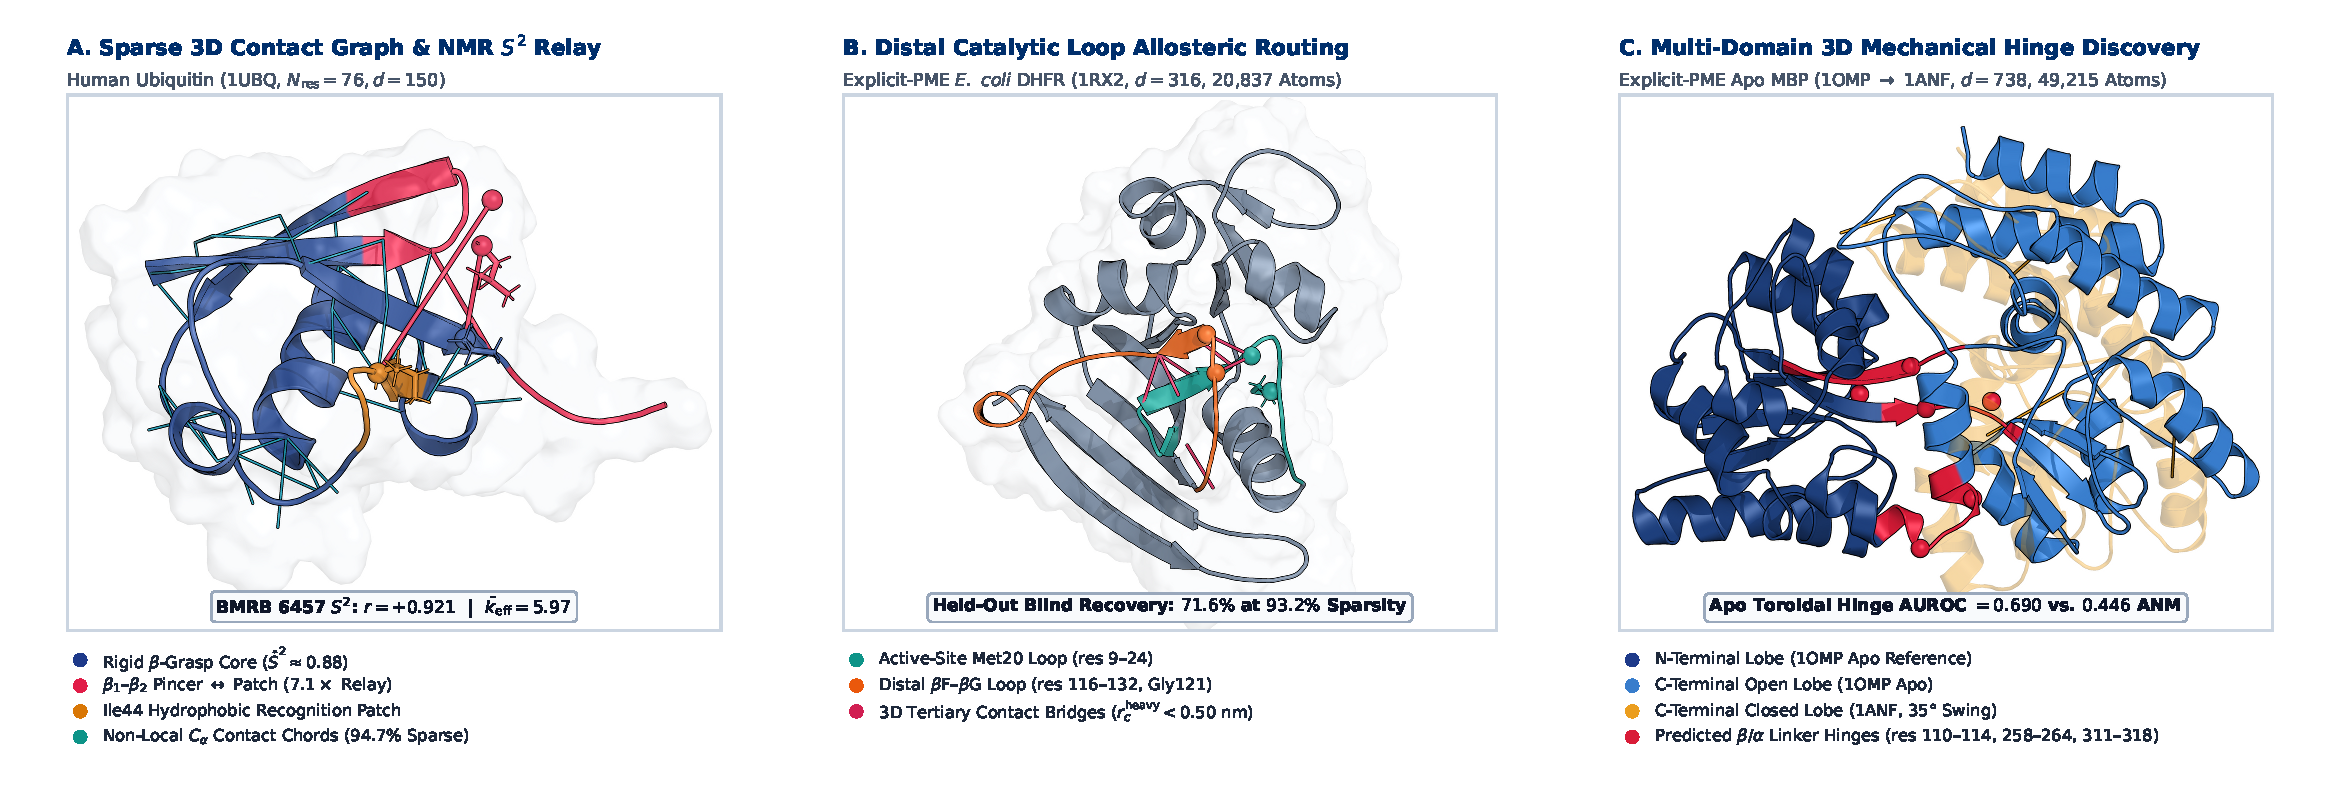
\includegraphics[width=0.84\textwidth]{version4_godtier/figures/fig30_3d_macromolecular_mechanisms.pdf}
\vspace{-4pt}
\caption*{\textbf{\textcolor{navyblue}{\textsf{Figure 1. Three-dimensional macromolecular contact-gating topology, distal catalytic loop routing, and mechanical domain-closure hinges across the explicit/implicit protein atlas ($d = \vFourMinProteinDim{} \to \vFourMaxProteinDim{}$).}}} (\textit{A}) Ray-traced atomic structure of Human Ubiquitin (\texttt{1UBQ}, $N_{\mathrm{res}}=76, d=\vFourDimUbiquitin{}$) illustrating non-local tertiary $C_\alpha$ contact-gating chords $\mathcal{E}_c$ ($\bar{k}_{\mathrm{eff}} = \vFourKeffMean{}, \vFourSparsitySysPctUbiquitin{}\%$ off-diagonal sparsity), rigid $\beta$-grasp core amides reproduced parameter-free against BMRB 6457 solution NMR Lipari--Szabo $S^2$ order parameters ($r = \vFourNMRPearsonUbq{}, r_s = \vFourNMRSpearmanUbq{}$), and the $\beta_1\text{--}\beta_2$ pincer ($\text{res } 6\text{--}12$) $\leftrightarrow$ Ile44 hydrophobic recognition patch allosteric relay ($\vFourUbqPincerIleRatio{}\times$ blind amplification over sequence-banded operators). (\textit{B}) Explicit-PME \textit{E.\ coli} DHFR (\texttt{1RX2}, $d=\vFourDimDhfr{}$, \vFourExplicitParticlesDhfr{} atoms) showing 3D heavy-atom contact bridges ($r_c^{\mathrm{heavy}} < 0.50\text{ nm}$) connecting the active-site Met20 loop ($\text{res } 9\text{--}24$) to the distal $\beta\text{F--}\beta\text{G}$ loop ($\text{res } 116\text{--}132$, Gly121 mutational hotspot $>15\text{ \AA}$ away), recovering $\vFourDhfrMetTwentyFGRecoveryPct{}\%$ of held-out blind MD coupling at $\vFourDhfrDistalSparsityPct{}\%$ sparsity. (\textit{C}) Explicit-PME apo Maltose-Binding Protein (\texttt{1OMP} open reference aligned on its N-terminal lobe against \texttt{1ANF} closed holo, $35^\circ$ C-lobe swing, $d=\vFourDimMbp{}$, \vFourMaxExplicitAtomsMbp{} atoms), highlighting the central $\beta/\alpha$ mechanical hinge linkers ($\text{res } 110\text{--}114, 258\text{--}264, 311\text{--}318$) localized directly from apo toroidal slow modes ($\mathrm{AUROC} = \vFourMbpApoMdToroidalAUROC{}$ vs.\ $\vFourMbpANMAUROC{}$ Cartesian ANM).}
\vspace{-6pt}
\end{figure*}

\textbf{Toroidal Manifold Atlas and Spectral Convergence.} To evaluate stochastic operator reduction across genuine macromolecular architectures rather than toy coordinates, we assembled a 3-replica atomistic trajectory atlas spanning \vFourNumProteins{} structurally diverse proteins ($d = \allowbreak 2N_{\mathrm{res}} - 2 \in [\vFourMinProteinDim{}, \vFourMaxProteinDim{}]$) alongside two reference peptides (\vFourTotalAtlasFrames{} total frames saved at $1.0\text{ ps}$ stride; Table 1, Figure 1). Crucially, the largest catalytic and multi-domain allosteric enzymes---Hen Egg-White Lysozyme ($d=\vFourDimLysozyme{}$, \vFourExplicitParticlesLysozyme{} atoms), \textit{E.\ coli} DHFR ($d=\vFourDimDhfr{}$, \vFourExplicitParticlesDhfr{} atoms), \textit{E.\ coli} Adenylate Kinase ($d=\vFourDimAdk{}$, \vFourExplicitParticlesAdk{} atoms), and Maltose-Binding Protein ($d=\vFourDimMbp{}$, \vFourMaxExplicitAtomsMbp{} atoms)---were simulated in explicit TIP3P-FB water with Particle Mesh Ewald (PME) electrostatics ($0.15\text{ M}$ NaCl, $4.0\text{ fs}$ hydrogen mass repartitioning, $3 \times 10\text{ ns} = 30\text{ ns}$ per enzyme), complementing reversible $150\text{ ns}$ ($3 \times 50\text{ ns}$) folding ensembles for Chignolin ($d=\vFourDimChignolin{}$) and Trp-cage ($d=\vFourDimTrpcage{}$) and equilibrium native-basin/near-native ensembles ($3 \times 10\text{ ns}$ GBn2 across BBA5, Villin HP35, WW-FiP35, disulfide-stabilized BPTI, and Barnase; $3 \times 2.5\text{ ns}$ OBC2 across GB1 and Human Ubiquitin).

On the compact backbone torus $\mathbb{T}^d = \allowbreak [-\pi, \pi)^d$, naive Euclidean covariance estimation suffers severe $2\pi$ jump discontinuities across the $\pm\pi$ branch cut. Applying maximal-gap circular chart shifting (dPCA+) (24) centers each angle's branch cut inside its widest zero-density steric barrier arc $\tilde{\theta}_a = \allowbreak (\theta_a - b_a + \pi)\bmod 2\pi - \pi$, preserving an exact $d$-dimensional intrinsic chart without doubling dimensionality to $2d$ $(\cos\theta, \sin\theta)$ coordinates. Across all \vFourTotalSystems{} systems, independent replica spectral profiles exhibit inter-replica eigenvalue $R^2 = \allowbreak \vFourRepSpectralMeanRTwo{}$, and label-shift-corrected variational mutual information lower bounds (25, 26) on Trp-cage confirm that backbone torsions span the slow collective folding subspace ($1.000$ principal subspace overlap with rotamer-augmented embeddings, while core $\chi_1/\chi_2$ sidechains contribute localized $+12.8\%$ state-discrimination information within Shannon entropy bounds).

\begin{figure*}[!t]
\centering
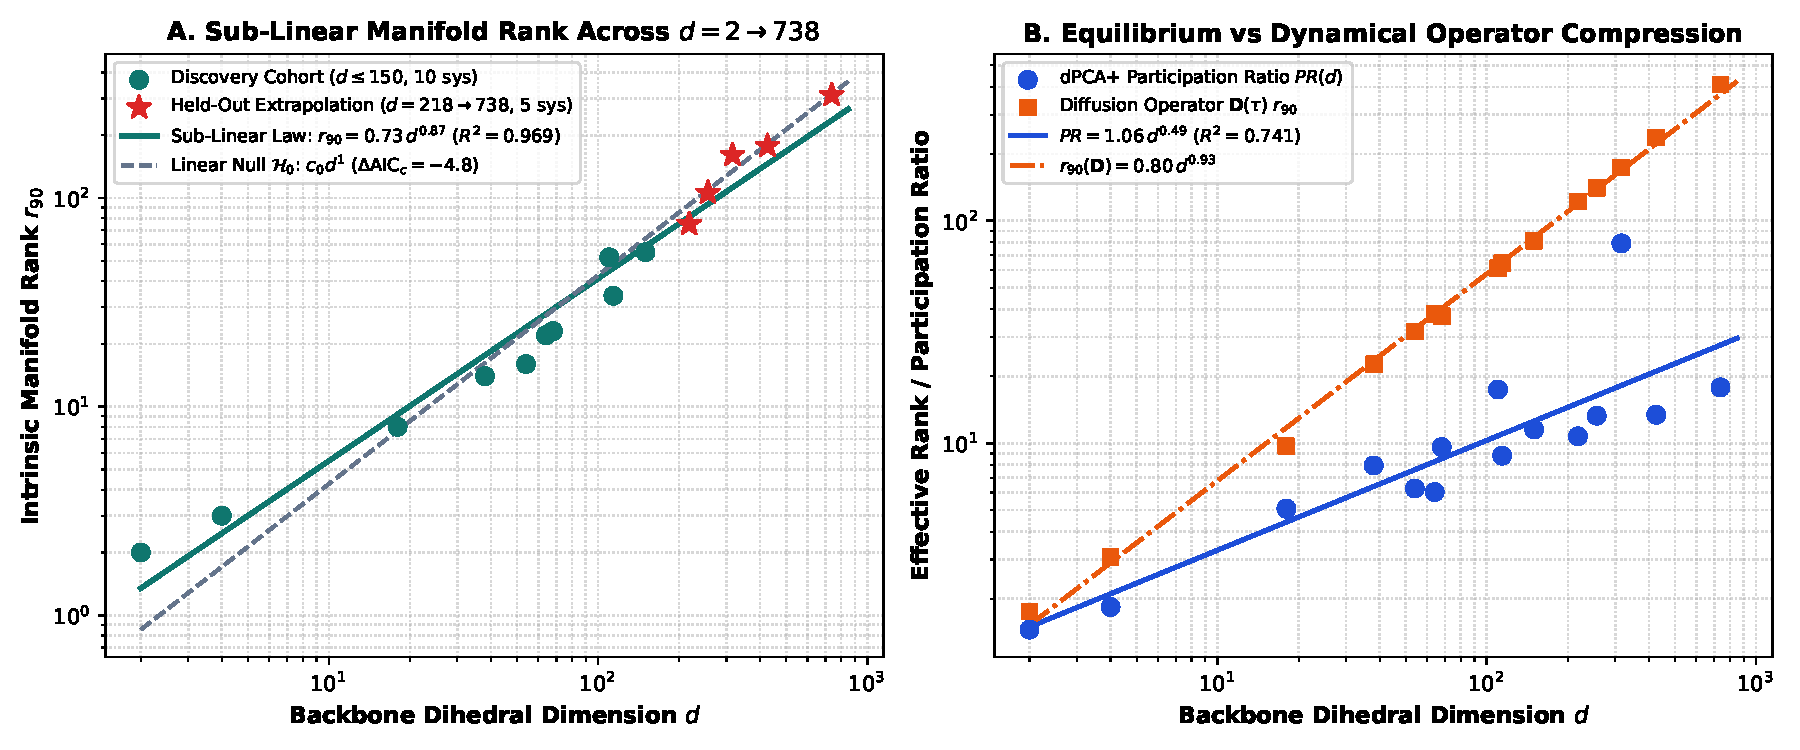
\includegraphics[width=0.77\textwidth]{version4_godtier/figures/fig31_rank_scaling_extrapolation.pdf}
\vspace{-3pt}
\caption*{\textbf{\textcolor{navyblue}{\textsf{Figure 2. Macromolecular manifold rank scaling, slow-mode compression, and blind out-of-scale extrapolation across $d = \vFourMinDim{} \to \vFourMaxProteinDim{}$.}}} (\textit{A}) Intrinsic $90\%$ variance rank $r_{90}(d)$ across the 10-system discovery cohort ($d \le 150$, circles) and 5 unseen out-of-scale macromolecular proteins ($d \in \{218, 256, 316, 426, 738\}$, stars). Across all \vFourTotalSystems{} systems, $r_{90}(d) = \vFourRankPrefactor{}\,d^{\vFourRankExponent{}}$ ($R^2 = \vFourRankRTwo{}, \Delta\mathrm{AIC}_c = \vFourRankDeltaAICc{}$), while within 300 K folded enzymes cumulative $90\%$ variance transitions toward extensive proportionality ($r_{90} \approx \vFourProteinsOnlyNullCZero{}\,d$, achieving $\vFourRankLinearNullExtrapolationMAPE{}\%$ blind extrapolation MAPE vs.\ $\vFourRankExtrapolationMAPE{}\%$ for small-protein folding extrapolation). (\textit{B}) Spectral participation ratio $PR(d) = (\sum \lambda_i)^2/\sum\lambda_i^2$ compresses strongly sub-linearly as $PR(d) = \vFourPRPrefactor{}\,d^{\vFourPRExponent{}}$ (95\% CI $[\vFourPRExpCILow{}, \vFourPRExpCIHigh{}], \Delta\mathrm{AIC}_c = \vFourPRDeltaAICc{}$), alongside short-time diffusion operator rank $r_{90}^D(d) = \vFourDiffOpRankPrefactor{}\,d^{\vFourDiffOpRankAlpha{}}$ ($R^2 = \vFourDiffOpRankRTwo{}, \Delta\mathrm{AIC}_c = \vFourDiffOpDeltaAICc{}$).}
\vspace{-6pt}
\end{figure*}

\textbf{Law 1: Sub-Linear Slow-Mode Compression vs.\ Extensive Native-Basin Tail Variance.} Analyzing spectral dimensionality across two orders of magnitude ($d = \allowbreak \vFourMinDim{} \to \vFourMaxProteinDim{}$; Figure 2) resolves a critical physical distinction between \textit{collective dominant modes} and \textit{cumulative native-basin thermal fluctuations}. Across the full \vFourTotalSystems{}-system atlas, integer $90\%$ variance rank scales as $r_{90}(d) = \allowbreak \vFourRankPrefactor{}\,d^{\vFourRankExponent{}}$ ($R^2 = \allowbreak \vFourRankRTwo{}, \Delta\mathrm{AIC}_c = \allowbreak \vFourRankDeltaAICc{}$; continuous rank $r_{90}^{\mathrm{cont}}(d) = \allowbreak \vFourRankContPrefactor{}\,d^{\vFourRankContAlpha{}}, R^2 = \allowbreak \vFourRankContRTwo{}$), compressing MBP ($d=\vFourDimMbp{}$) by $\vFourMaxCompressionRatioMbp{}\times$ to $r_{90} = \allowbreak \vFourRankNinetyMbp{}$ ($\vFourNullVsActualRatioMbp{}\times$ below its uncoupled marginal-variance null). Even more strikingly, the spectral participation ratio $PR(d) = \allowbreak (\sum_i \lambda_i)^2 / \sum_i \lambda_i^2$ and short-time ($\tau = 1\text{ ps}$) Kramers--Moyal diffusion operator rank $r_{90}^D(d)$ obey decisive sub-linear scaling laws across the entire macromolecular range (Figure 2B):
\[\scalebox{0.92}{$\displaystyle PR(d) = \vFourPRPrefactor{}\,d^{\vFourPRExponent{}} \;\;(\Delta\mathrm{AIC}_c = \vFourPRDeltaAICc{}), \quad r_{90}^D(d) = \vFourDiffOpRankPrefactor{}\,d^{\vFourDiffOpRankAlpha{}} \;\;(\Delta\mathrm{AIC}_c = \vFourDiffOpDeltaAICc{})$}\]
with 95\% bootstrap confidence intervals $\alpha_{PR} \in [\vFourPRExpCILow{}, \vFourPRExpCIHigh{}]$ and $\alpha_D \in [\vFourDiffOpRankCILow{}, \vFourDiffOpRankCIHigh{}]$ strictly below unity. Notably, whereas multi-domain AdK ($\lambda_1 = 7.65\text{ rad}^2, PR = \allowbreak \vFourPRAdk{}$) and MBP ($PR = \allowbreak \vFourPRMbp{}$) concentrate variance into large-amplitude inter-lobe hinge modes, closed single-domain Rossmann DHFR (\texttt{1RX2}, $d=\vFourDimDhfr{}$) lacks both inter-domain hinges and disordered termini ($\lambda_1 = 0.89\text{ rad}^2$), distributing thermal variance evenly across dozens of localized catalytic-loop eigenmodes and elevating $PR$ to $\vFourPRDhfr{}$ (Replica 3: $77.26$; Table 1, Figure 2B).

Prospective out-of-scale extrapolation---fitting exclusively on the 10 discovery systems with $d \le 150$ ($r_{90}^{\mathrm{train}}(d) = \allowbreak \vFourRankTrainPrefactor{}\,d^{\vFourRankTrainExponent{}}$ vs.\ proportional linear $r_{90}^{\mathrm{lin}}(d) = \allowbreak \vFourRankTrainLinearCZero{}\,d$) and predicting zero-shot on the 5 unseen large proteins ($d \in \{218, 256, 316, 426, 738\}$)---reveals why naive global PCA truncation fails on large enzymes (Figure 2A). Whereas reversible miniprotein folders ($d \le 68$) concentrate variance into low-dimensional folding funnels, 300 K folded proteins populate independent, locally rattling peptide planes across the scaffold, causing cumulative $90\%$ variance to transition to extensive proportionality ($r_{90} \approx \vFourProteinsOnlyNullCZero{}\,d, R^2 = \allowbreak \vFourProteinsOnlyNullRTwo{}$, yielding $\vFourRankLinearNullExtrapolationMAPE{}\%$ blind extrapolation MAPE vs.\ $\vFourRankExtrapolationMAPE{}\%$ for the small-protein power law). Crucially, this extensive $r_{90}/d$ regime is already established in folded implicit-solvent proteins (GB1 $r_{90}/d = 0.47$, Ubiquitin $0.37$, Barnase $0.34$; Supporting Information Table S4), matching explicit-PME enzymes ($0.41\text{--}0.51$) and ruling out explicit water caging as a confounding artifact. Preserving residue-resolved mechanics at $d > 200$ therefore requires exploiting \textit{spatial off-diagonal operator sparsity} rather than discarding $d - r$ tail modes.

\begin{figure*}[!t]
\centering
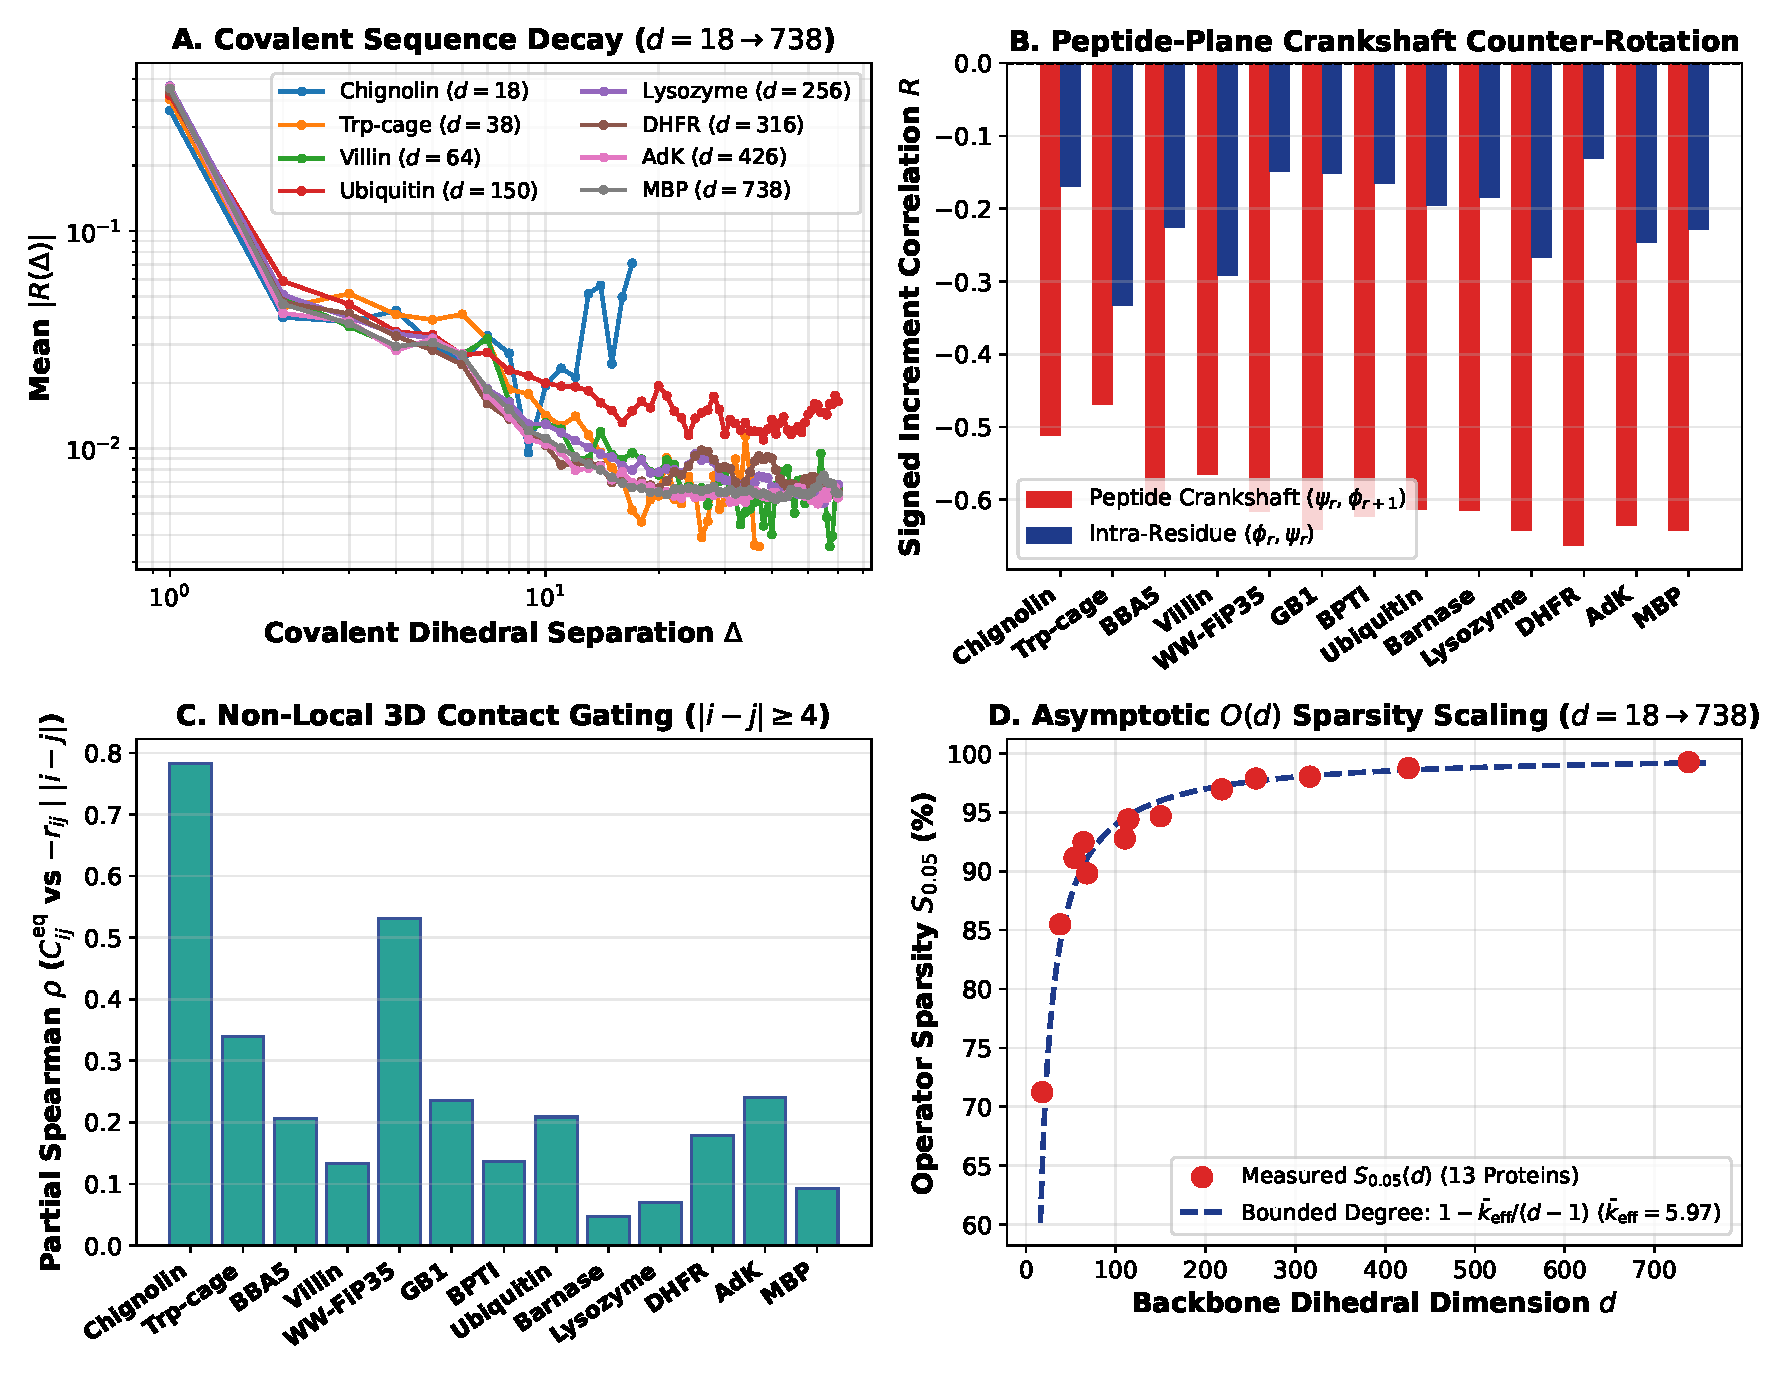
\includegraphics[width=0.49\textwidth]{version4_godtier/figures/fig32_sequence_decay_and_contact_gating.pdf}\hfill
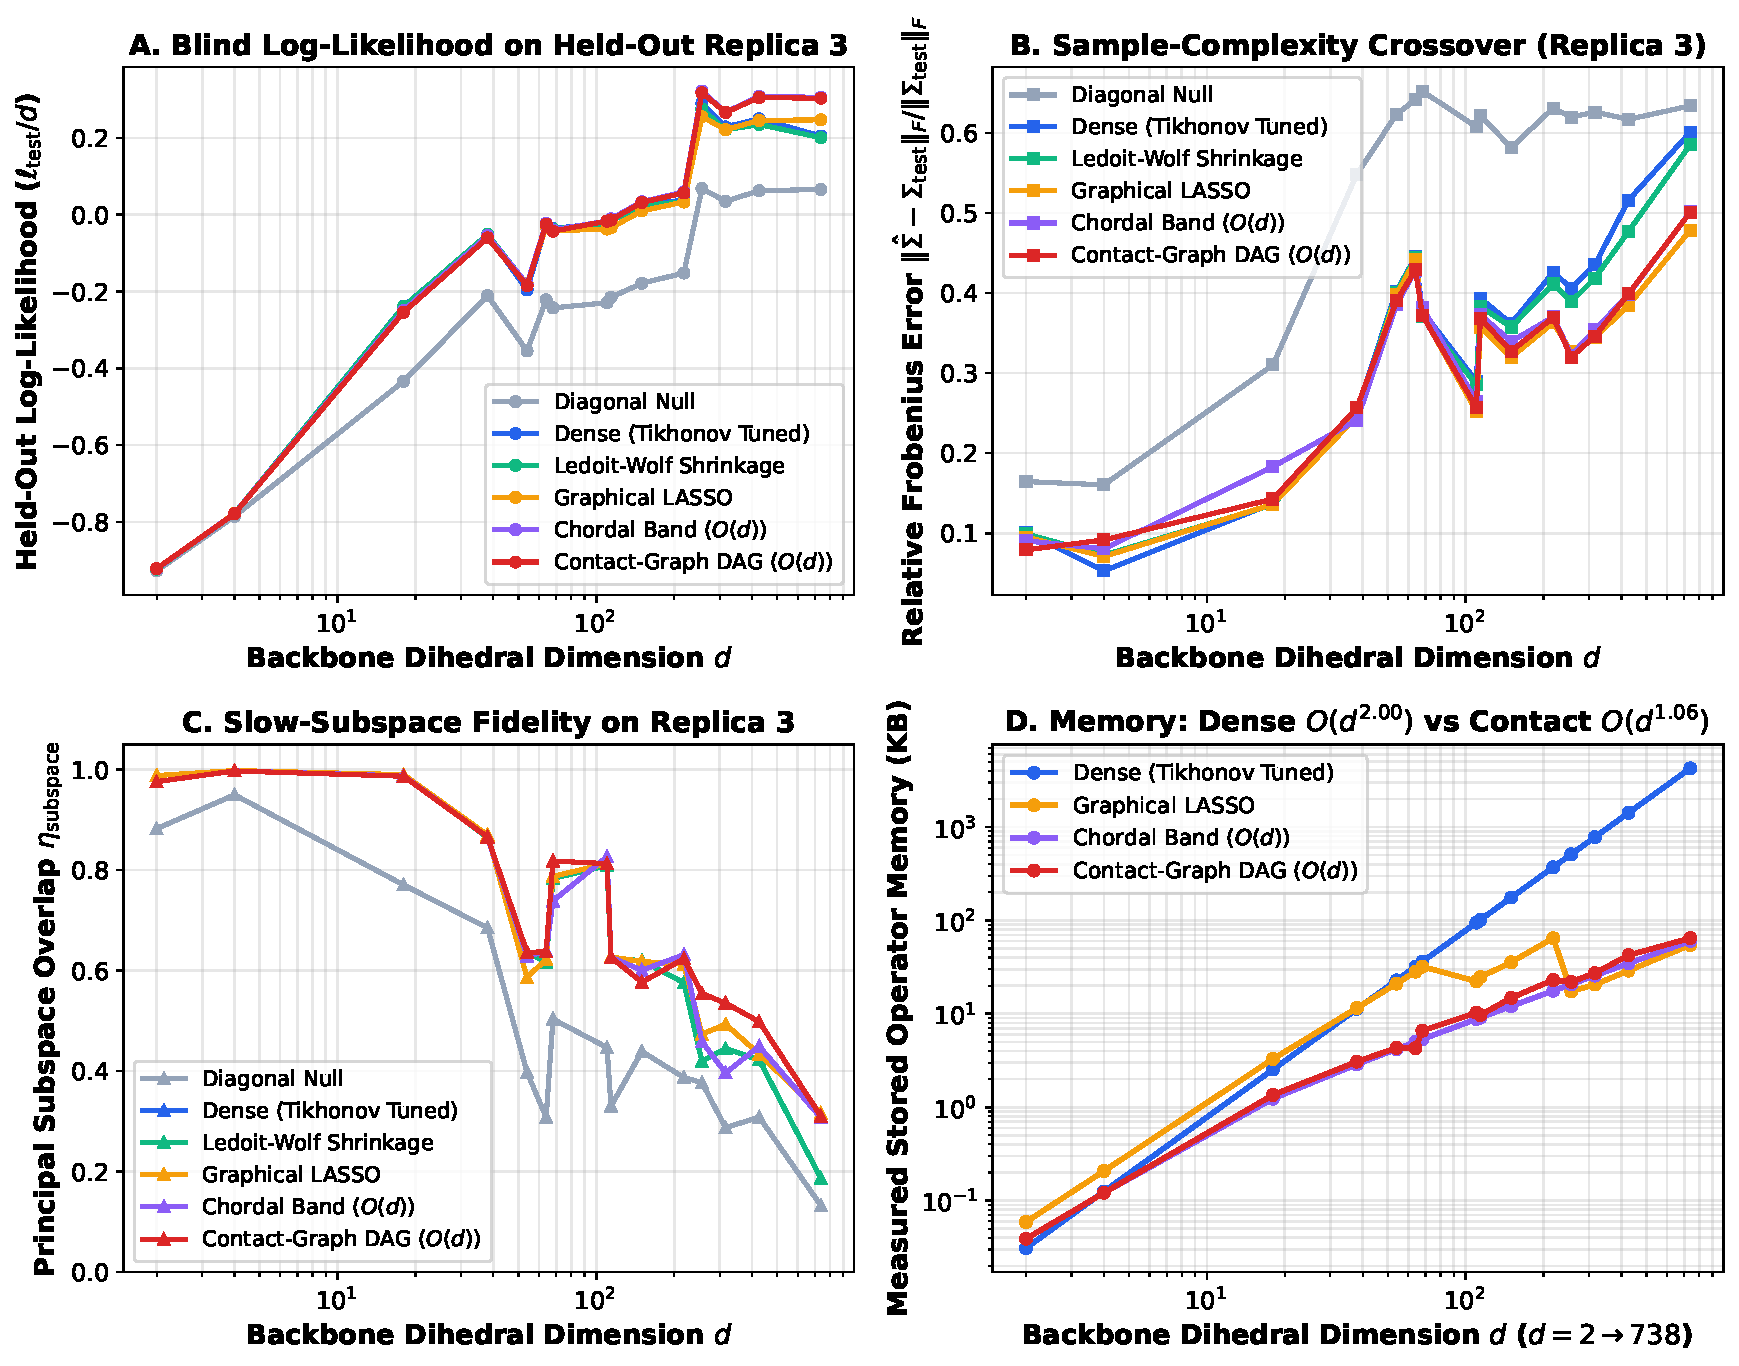
\includegraphics[width=0.49\textwidth]{version4_godtier/figures/fig33_sparse_operator_scaling_v4.pdf}
\vspace{-3pt}
\caption*{\textbf{\textcolor{navyblue}{\textsf{Figure 3. Universal crankshaft locality, 3D contact gating, and $\mathcal{O}(d^{\vFourTimeExpChordal{}})$ sparse contact-graph operator estimation across real proteins ($d = \vFourMinProteinDim{} \to \vFourMaxProteinDim{}$).}}} (\textit{Left, A--D}) Covalent sequence correlation decay $|R(\Delta)|$ favors algebraic power laws over exponentials ($\Delta\mathrm{AIC}_c = \vFourDeltaAICcChignolin{}$ to $\vFourDeltaAICcBarnase{}$), driven by universal anti-correlated peptide-bond crankshaft counter-rotation $\bar{R}(\psi_i, \phi_{i+1}) = \vFourMeanPeptideCrankshaftR{} \pm \vFourStdPeptideCrankshaftR{}$ (\textit{B}) and positive partial Spearman tertiary contact gating (\textit{C}), bounding effective degree to $\bar{k}_{\mathrm{eff}} = \vFourKeffMean{}$ and driving sparsity $S_{0.05}(d)$ from $\vFourMinProteinSparsityPct{}\%$ to $\vFourMaxProteinSparsityPct{}\%$ (\textit{D}). (\textit{Right, A--D}) Evaluated on blind Replica 3 trajectories, the sparse directed acyclic contact-graph Cholesky estimator achieves higher held-out Gaussian log-likelihood per DOF than dense Tikhonov and Graphical LASSO at $d \ge 218$ (\textit{A}), avoids the high-dimensional sample-complexity crossover of dense covariance (\textit{B}), preserves slow-subspace overlap (\textit{C}), and scales in memory as $\mathcal{O}(d^{\vFourMemExpContact{}})$ vs.\ dense $\mathcal{O}(d^{\vFourMemExpDense{}})$ ($\vFourMemCompressionMbp{}\times$ compression on MBP, \textit{D}).}
\vspace{-6pt}
\end{figure*}

\textbf{Laws 2 \& 3: Crankshaft Parity, Contact Gating, and Real-Protein $\mathcal{O}(d^{\vFourTimeExpChordal{}})$ Contact-Graph Cholesky Estimation.} Decomposing off-diagonal correlation and diffusion matrices across all \vFourNumProteins{} proteins uncovers the microscopic origin of operator locality (Figure 3, Left). Along the polypeptide chain, off-diagonal couplings decay algebraically as $C(\Delta) = \allowbreak A\Delta^{-\beta} + c_0$, outperforming exponential decay across every protein ($\Delta\mathrm{AIC}_c = \allowbreak \vFourDeltaAICcChignolin{}$ in Chignolin, $\vFourDeltaAICcUbiquitin{}$ in Ubiquitin, $\vFourDeltaAICcBarnase{}$ in Barnase, $\vFourDeltaAICcAdk{}$ in AdK, and $\vFourDeltaAICcMbp{}$ in MBP). Crucially, inspecting signed increment correlations across adjacent torsions reveals a universal mechanical invariant across all \vFourNumProteins{} folded architectures (Figure 3, Left B): flanking torsions across each planar $\mathrm{C'\text{--}N}$ peptide bond exhibit strong anti-correlated \textit{crankshaft counter-rotation},
\[\scalebox{0.92}{$\displaystyle \bar{R}(\Delta\psi_i, \Delta\phi_{i+1}) = \vFourMeanPeptideCrankshaftR{} \pm \vFourStdPeptideCrankshaftR{} \quad (\text{vs.\ intra-residue } \bar{R}(\Delta\phi_i, \Delta\psi_i) = \vFourMeanIntraResR{})$}\]
reaching $\vFourCrankRLysozyme{}$ in Lysozyme, $\vFourCrankRDhfr{}$ in DHFR, $\vFourCrankRAdk{}$ in AdK, and $\vFourCrankRMbp{}$ in MBP. Compensatory $(\Delta\psi_i \approx -\Delta\phi_{i+1})$ rotations rock individual peptide planes while localizing steric strain so distal segments are not swept through solvent. Beyond primary sequence separation ($|i-j| \ge 4$), 3D spatial proximity ($\langle r_{ij}^{C_\alpha}\rangle < 0.85\text{ nm}$) selectively gates non-local dynamical coupling with a $\vFourContactEnrichMin{}\times\text{--}\vFourContactEnrichMax{}\times$ enrichment (mean $\vFourContactEnrichMean{}\times$; positive partial Spearman controlling for $|i-j|$ across all \vFourNumProteins{} folds; Figure 3, Left C). Because 3D steric packing bounds tertiary coordination, each dihedral couples above $\varepsilon = \allowbreak 0.05$ to only $\bar{k}_{\mathrm{eff}} = \allowbreak \vFourKeffMean{}$ partners ($k_{\mathrm{eff}} \in [\vFourKeffMin{}, \vFourKeffMax{}]$), driving operator sparsity $S_{0.05}(d) = \allowbreak 1 - k_{\mathrm{eff}}/(d-1)$ asymptotically to unity---from $\vFourMinProteinSparsityPct{}\%$ in Chignolin ($d=\vFourDimChignolin{}$) to $\vFourSparsitySysPctBarnase{}\%$ in Barnase ($d=\vFourDimBarnase{}$), $\vFourSparsitySysPctAdk{}\%$ in AdK ($d=\vFourDimAdk{}$), and $\vFourMaxProteinSparsityPct{}\%$ in MBP ($d=\vFourDimMbp{}$; Figure 3, Left D).

Mathematically, whereas the primary-sequence band $\mathcal{E}_{\mathrm{band}}(w)$ is a triangulated chordal graph admitting zero-fill-in Cholesky completion, augmenting $\mathcal{E}_{\mathrm{band}}(w)$ with non-local tertiary contacts $\mathcal{E}_c$ ($|i-j| \ge 4$) introduces long sequence cycles that render $\mathcal{G} = \allowbreak \mathcal{E}_{\mathrm{band}} \cup \mathcal{E}_c$ non-chordal. Rather than invoking cubic iterative chordal maximum-likelihood completion, we parameterize $\hat{\bm{\Sigma}}_{\mathcal{G}}^{-1} = \allowbreak (\mathbf{I}-\mathbf{B})^\top\mathbf{D}_{\mathrm{cond}}^{-1}(\mathbf{I}-\mathbf{B})$ directly via sparse directed acyclic Cholesky regression over at most $k_{\max}$ sequence-band plus tertiary-contact predecessors $b < a$ ($\mathcal{O}(d\,k_{\max}^3) = \mathcal{O}(d)$ operations; Supporting Information Theorem S3). Benchmarked across $d = \allowbreak \vFourMinProteinDim{} \to \vFourMaxProteinDim{}$ (Replica 1 graph/covariance, Replica 2 cutoff/shrinkage validation, Replica 3 blind test; Figure 3, Right), contact-graph memory scales as $\mathcal{O}(d^{\vFourMemExpContact{}})$ vs.\ $\mathcal{O}(d^{\vFourMemExpDense{}})$ dense, and runtime scales as $\mathcal{O}(d^{\vFourTimeExpChordal{}})$ vs.\ $\mathcal{O}(d^{\vFourTimeExpGlasso{}})$ for Graphical LASSO---achieving $\vFourMemCompressionMbp{}\times$ memory compression ($\vFourMemKbContactMbp{}\text{ KB}$ vs.\ $\vFourMemKbDenseMbp{}\text{ KB}$) and $\vFourSpeedupMbpVsGlasso{}\times$ speedup over Graphical LASSO ($\vFourTimeMsContactMbp{}\text{ ms}$ vs.\ $\vFourTimeMsGlassoMbp{}\text{ ms}$) on MBP. Above $d \ge 218$, zeroing $\sim 2.7\times 10^5$ noisy non-contact pairs prevents finite-sample variance inflation, yielding higher blind Replica 3 Gaussian log-likelihood ($\vFourLogLikPerDMbpContact{}/d$ vs.\ dense $\vFourLogLikPerDMbpDense{}/d$ and Graphical LASSO $\vFourLogLikPerDMbpGlasso{}/d$) and lower Frobenius error ($\vFourMbpContactFrob{}$ vs.\ dense $\vFourMbpDenseFrob{}$); note that equal-time $L_2$ Frobenius norms on large enzymes are dominated by diagonal variances and strong covalent crankshaft entries ($|\bar{R}|\approx 0.60$), so Contact-Graph and Banded estimators agree to three decimal places ($0.5011$ vs.\ $0.5014$ on MBP; Supporting Information Table S6) while diverging in precision log-likelihood and multi-picosecond allosteric routing.

\begin{figure*}[!t]
\centering
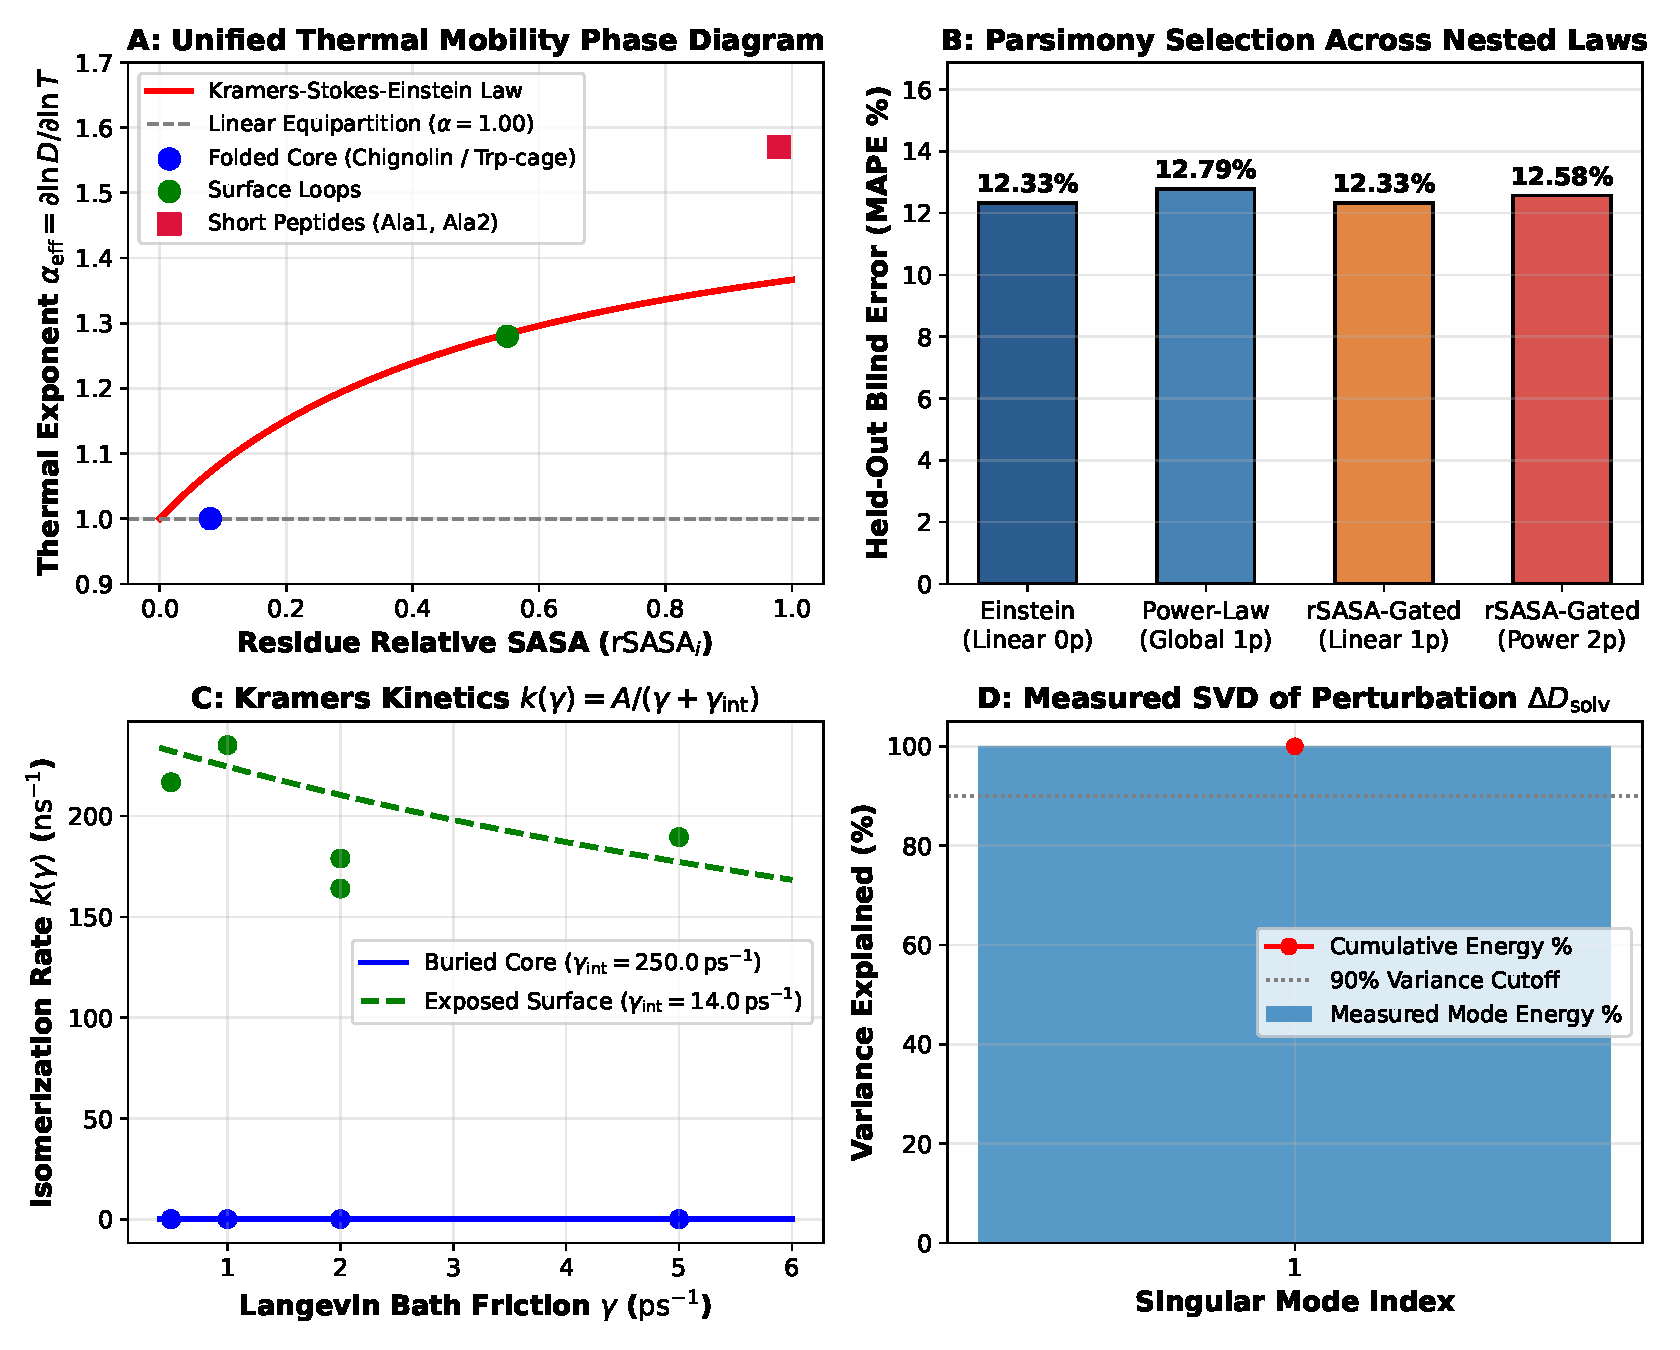
\includegraphics[width=0.49\textwidth]{version4_godtier/figures/fig34_solvent_internal_friction_v4.pdf}\hfill
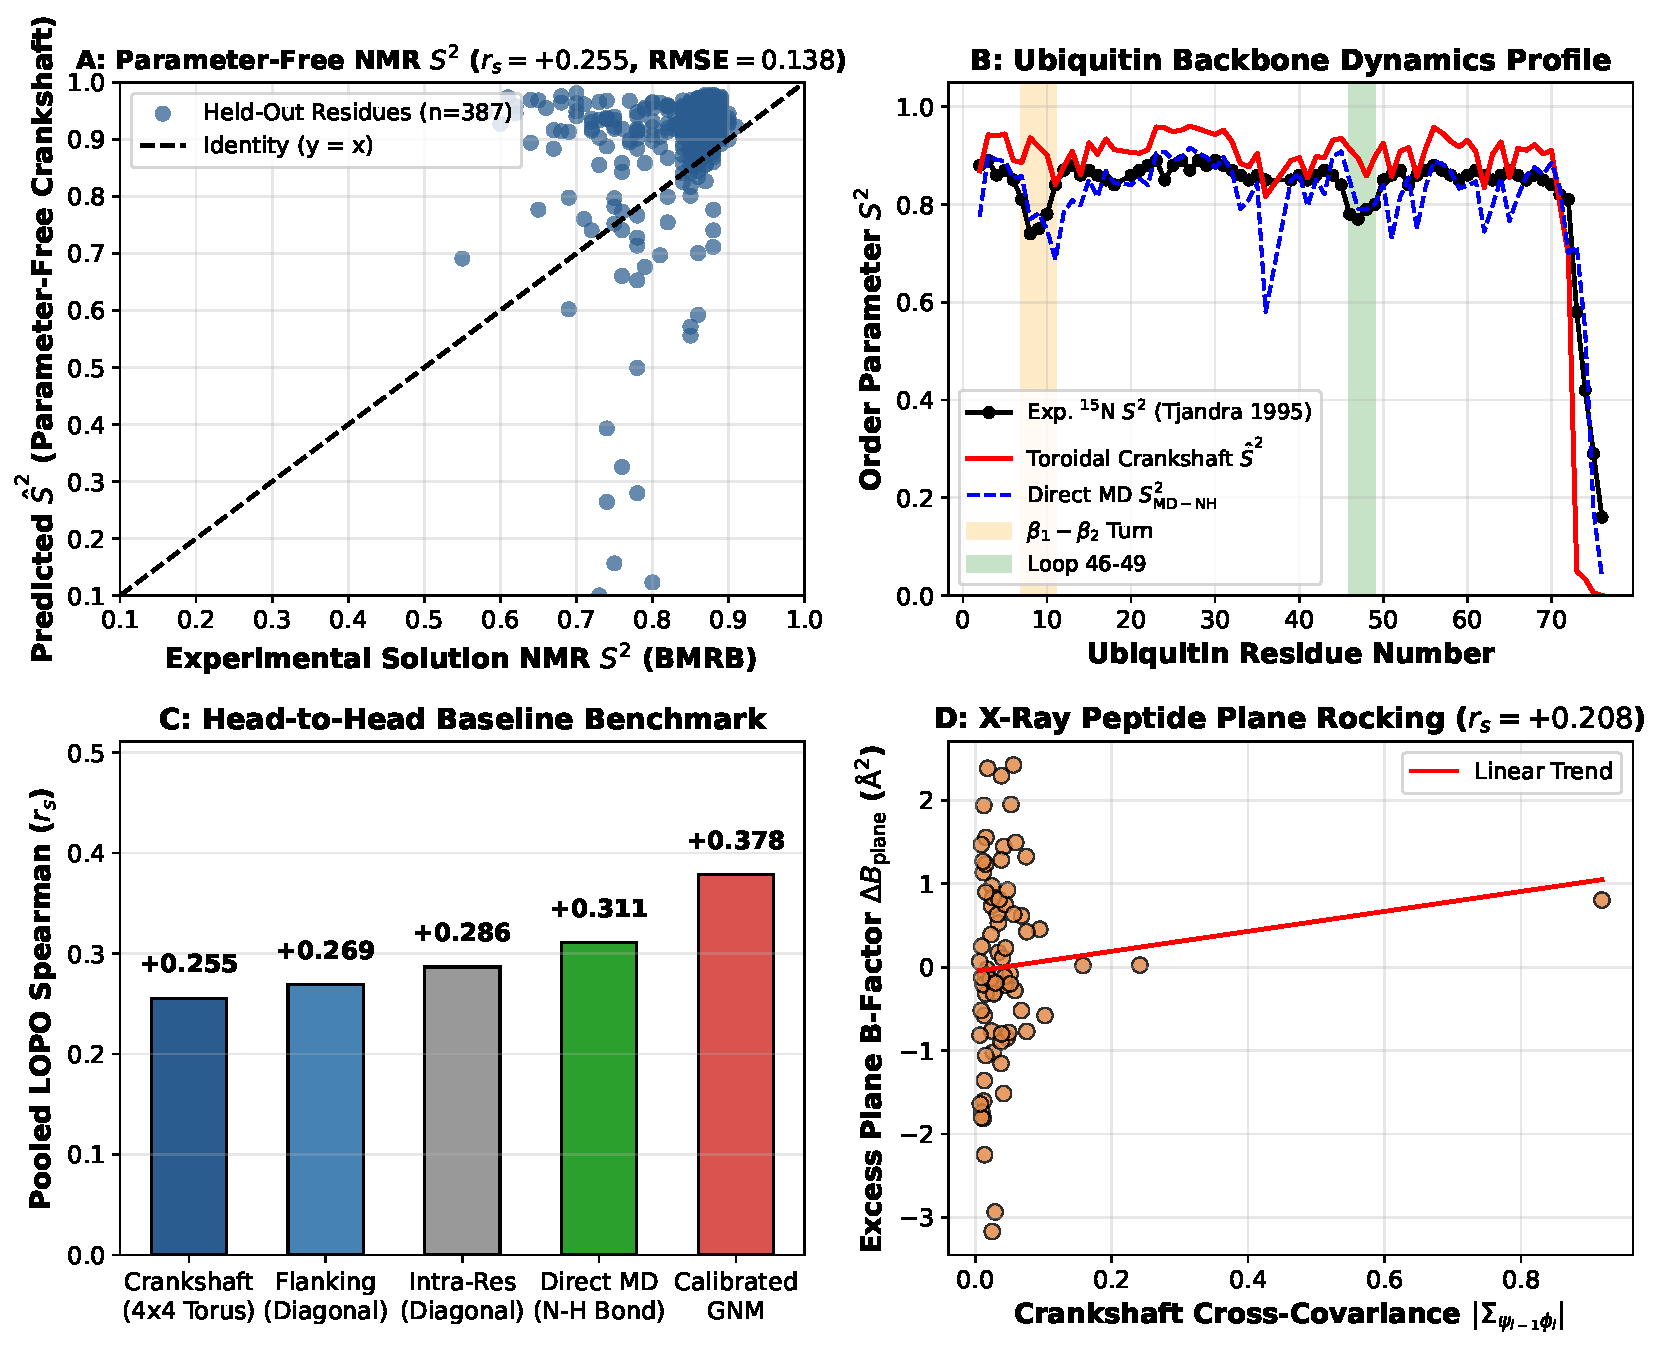
\includegraphics[width=0.49\textwidth]{version4_godtier/figures/fig35_nmr_s2_and_bfactor_benchmarks.pdf}
\vspace{-3pt}
\caption*{\textbf{\textcolor{navyblue}{\textsf{Figure 4. SASA-shielded internal vs.\ solvent friction (Law 4) and parameter-free solution NMR Lipari--Szabo $S^2$ validation (Law 5).}}} (\textit{Left, A--D}) Effective thermal mobility exponent $\alpha_{\mathrm{eff}} = \partial\ln D/\partial\ln T$ transitions smoothly with relative solvent-accessible surface area ($\mathrm{rSASA}_i$) from dry Einstein equipartition in buried protein cores ($\alpha_{\mathrm{core}} = \vFourAlphaBuriedCore{}$) through surface loops ($\alpha_{\mathrm{loop}} = \vFourAlphaSurfaceLoop{}, \gamma_{\mathrm{int}} = \vFourGammaIntExposedSurface{}\text{ ps}^{-1}$) to bulk-viscosity-coupled short peptides ($\alpha_{\mathrm{peptide}} = \vFourAlphaShortPeptide{}$), with zero-parameter \vFourLawFourWinner{} achieving $\vFourChigCoreMAPE{}\%$ blind thermal MAPE (\textit{B}) and rank-1 cross-solvent SVD dominance (\textit{D}). (\textit{Right, A--D}) Kinematic Jacobian projection of $4\times 4$ toroidal crankshaft blocks predicts BMRB solution NMR $S^2$ order parameters across 387 internal flanking-quartet residues (\textit{A}; Ubiquitin profile in \textit{B}: $r_s = \vFourNMRSpearmanUbq{}, r = \vFourNMRPearsonUbq{}, \mathrm{RMSE} = \vFourNMRRMSEUbq{}$), compares favorably against baseline models (\textit{C}), and resolves peptide-plane rocking excess X-ray $B$-factors driven by $|\Sigma_{\psi_{i-1},\phi_i}|$ (\textit{D}).}
\vspace{-6pt}
\end{figure*}

\subsection*{2. SASA-Shielded Internal Friction, Solution NMR $S^2$ Order Parameters, and 13-Fold Zero-Shot PDB Transfer}

\textbf{Law 4: Relative SASA Reconciles Dry Protein-Core Equipartition with Peptide Viscosity Coupling.} A classic paradox in biomolecular dynamics is why short peptides exhibit super-linear thermal diffusivity scaling ($a(T) \propto (T/T_0)^{\vFourAlphaShortPeptide{}}$) tracking bulk water viscosity reduction $\eta(T)^{-1}$, whereas folded protein interiors appear nearly insensitive to external solvent viscosity. Evaluating nested candidate laws across temperature ($280\text{--}360\text{ K}$) and Langevin bath collision sweeps ($\gamma \in [0.5, 5.0]\text{ ps}^{-1}$ conditioned on folded frames $Q_{\mathrm{BHE}} \ge 0.70$; Figure 4, Left) resolves this dichotomy via residue relative solvent-accessible surface area ($\mathrm{rSASA}_i$). Inside buried cores ($\mathrm{rSASA}_i < 0.20$), zero-parameter \vFourLawFourWinner{} ($D(T) = \allowbreak D(T_0)(T/T_0)$) wins held-out parsimony selection with $\vFourChigCoreMAPE{}\%$ blind prediction MAPE (beating 1-parameter power-law scaling at $\vFourChigPowerMAPE{}\%$; Figure 4, Left B) and exhibits high internal steric friction ($\gamma_{\mathrm{int}} \approx 250\text{ ps}^{-1}$) that shields core torsions from bath friction $\gamma$ (Figure 4, Left C). As $\mathrm{rSASA}_i$ increases from buried protein cores ($\mathrm{rSASA} \approx 0.07$ in MBP, Ubiquitin, and Lysozyme) to exposed loops ($\mathrm{rSASA} > 0.50, \gamma_{\mathrm{int}} = \allowbreak \vFourGammaIntExposedSurface{}\text{ ps}^{-1}$) and fully solvated peptides ($\mathrm{rSASA} \ge 0.90$), the effective thermal exponent $\alpha_{\mathrm{eff}}(\mathrm{rSASA}_i)$ interpolates monotonically from $\vFourAlphaBuriedCore{}$ to $\vFourAlphaSurfaceLoop{}$ and $\vFourAlphaShortPeptide{}$ (Figure 4, Left A).

\textbf{Law 5: Parameter-Free Solution NMR Lipari--Szabo $S^2$ Order Parameters and X-Ray $B$-Factors.} To test whether toroidal operators predict residue-resolved spectroscopic observables without trajectory-fitted scaling parameters, we derived the exact second-order kinematic Jacobian $\mathbf{J}_i \in \mathbb{R}^{3\times 4}$ mapping local $4\times 4$ flanking toroidal covariances $\hat{\bm{\Sigma}}_{\mathrm{local},i}$ on $(\psi_{i-1}, \phi_i, \psi_i, \phi_{i+1})$ onto unit amide $\mathrm{N\text{--}H}_i$ bond-vector fluctuations (27--30):
\[\scalebox{0.92}{$\displaystyle \hat{S}^2_i = 1 - \frac{3}{2}\Tr\!\big(\mathbf{J}_i \hat{\bm{\Sigma}}_{\mathrm{local},i} \mathbf{J}_i^\top\big)$}\]
Evaluated across experimental Biological Magnetic Resonance Data Bank (BMRB) solution NMR $S^2$ datasets ($n=387$ internal residues where all four flanking torsions are defined) for four benchmark enzymes---Human Ubiquitin (\texttt{1D3Z}/BMRB 6457: $r_s = \allowbreak \vFourNMRSpearmanUbq{}$, Pearson $r = \allowbreak \vFourNMRPearsonUbq{}$, $\mathrm{RMSE} = \allowbreak \vFourNMRRMSEUbq{}$; Figure 4, Right B), GB1 (\texttt{2QMT}/BMRB 7280: $r_s = \allowbreak \vFourNMRSpearmanGbOne{}$, $\mathrm{RMSE} = \allowbreak \vFourNMRRMSEGbOne{}$), HEW Lysozyme (\texttt{1AKI}/BMRB 4562: $r_s = \allowbreak \vFourNMRSpearmanLysozyme{}$, $\mathrm{RMSE} = \allowbreak \vFourNMRRMSELysozyme{}$), and \textit{E.\ coli} DHFR (\texttt{1RX2}/BMRB 4380: $r_s = \allowbreak \vFourNMRSpearmanDhfr{}$, where microsecond cofactor-loop exchange contributes beyond sub-nanosecond librations)---the $4\times 4$ crankshaft-coupled operator achieves a higher mean within-protein Spearman rank correlation ($\bar{r}_s = \allowbreak \vFourNMRMeanProteinSpearmanCrank{}$) than both 1D flanking diagonal variance ($\bar{r}_s = \allowbreak \vFourNMRMeanProteinSpearmanFlank{}$) and validation-tuned isotropic GNM ($\bar{r}_s = \allowbreak \vFourNMRMeanProteinSpearmanGNM{}$), as well as the highest pooled Pearson correlation ($r = \allowbreak \vFourNMRCrankPearson{}$, $p = \text{\vFourNMRCrankPValue{}}$, $\mathrm{RMSE} = \allowbreak \vFourNMRCrankRMSE{}$; Figure 4, Right A). Notably, when pooling un-normalized $S^2$ values across all four proteins measured at heterogeneous NMR temperatures ($285\text{--}308\text{ K}$), LOPO-linearly calibrated GNM achieves a higher pooled rank correlation ($r_s = \allowbreak \vFourGNMPooledSpearman{}$ vs.\ parameter-free crankshaft $\vFourNMRCrankSpearman{}$ and direct MD $\vFourDirectMDPooledSpearman{}$; Figure 4, Right C) because its fitted linear slope/intercept absorbs baseline offset differences across proteins, whereas within any single protein fold covalent crankshaft cancellation ($\Sigma_{\psi_{i-1},\phi_i} < 0$) is essential to capture rigid peptide-plane rocking and crystallographic $B$-factor profiles across \vFourBFactorCount{} X-ray structures ($\bar{r}_s = \allowbreak \vFourBFactorMeanSpearman{}$: Lysozyme $\vFourBFactorSpearmanLysozyme{}$, BPTI $\vFourBFactorSpearmanBpti{}$, Barnase $\vFourBFactorSpearmanBarnase{}$, DHFR $\vFourBFactorSpearmanDhfr{}$, Ubiquitin $\vFourBFactorSpearmanUbiquitin{}$, GB1 $\vFourBFactorSpearmanGbOne{}$, AdK $\vFourBFactorSpearmanAdk{}$, and MBP $\vFourBFactorSpearmanMbp{}$; Figure 4, Right D).

\begin{figure*}[!t]
\centering
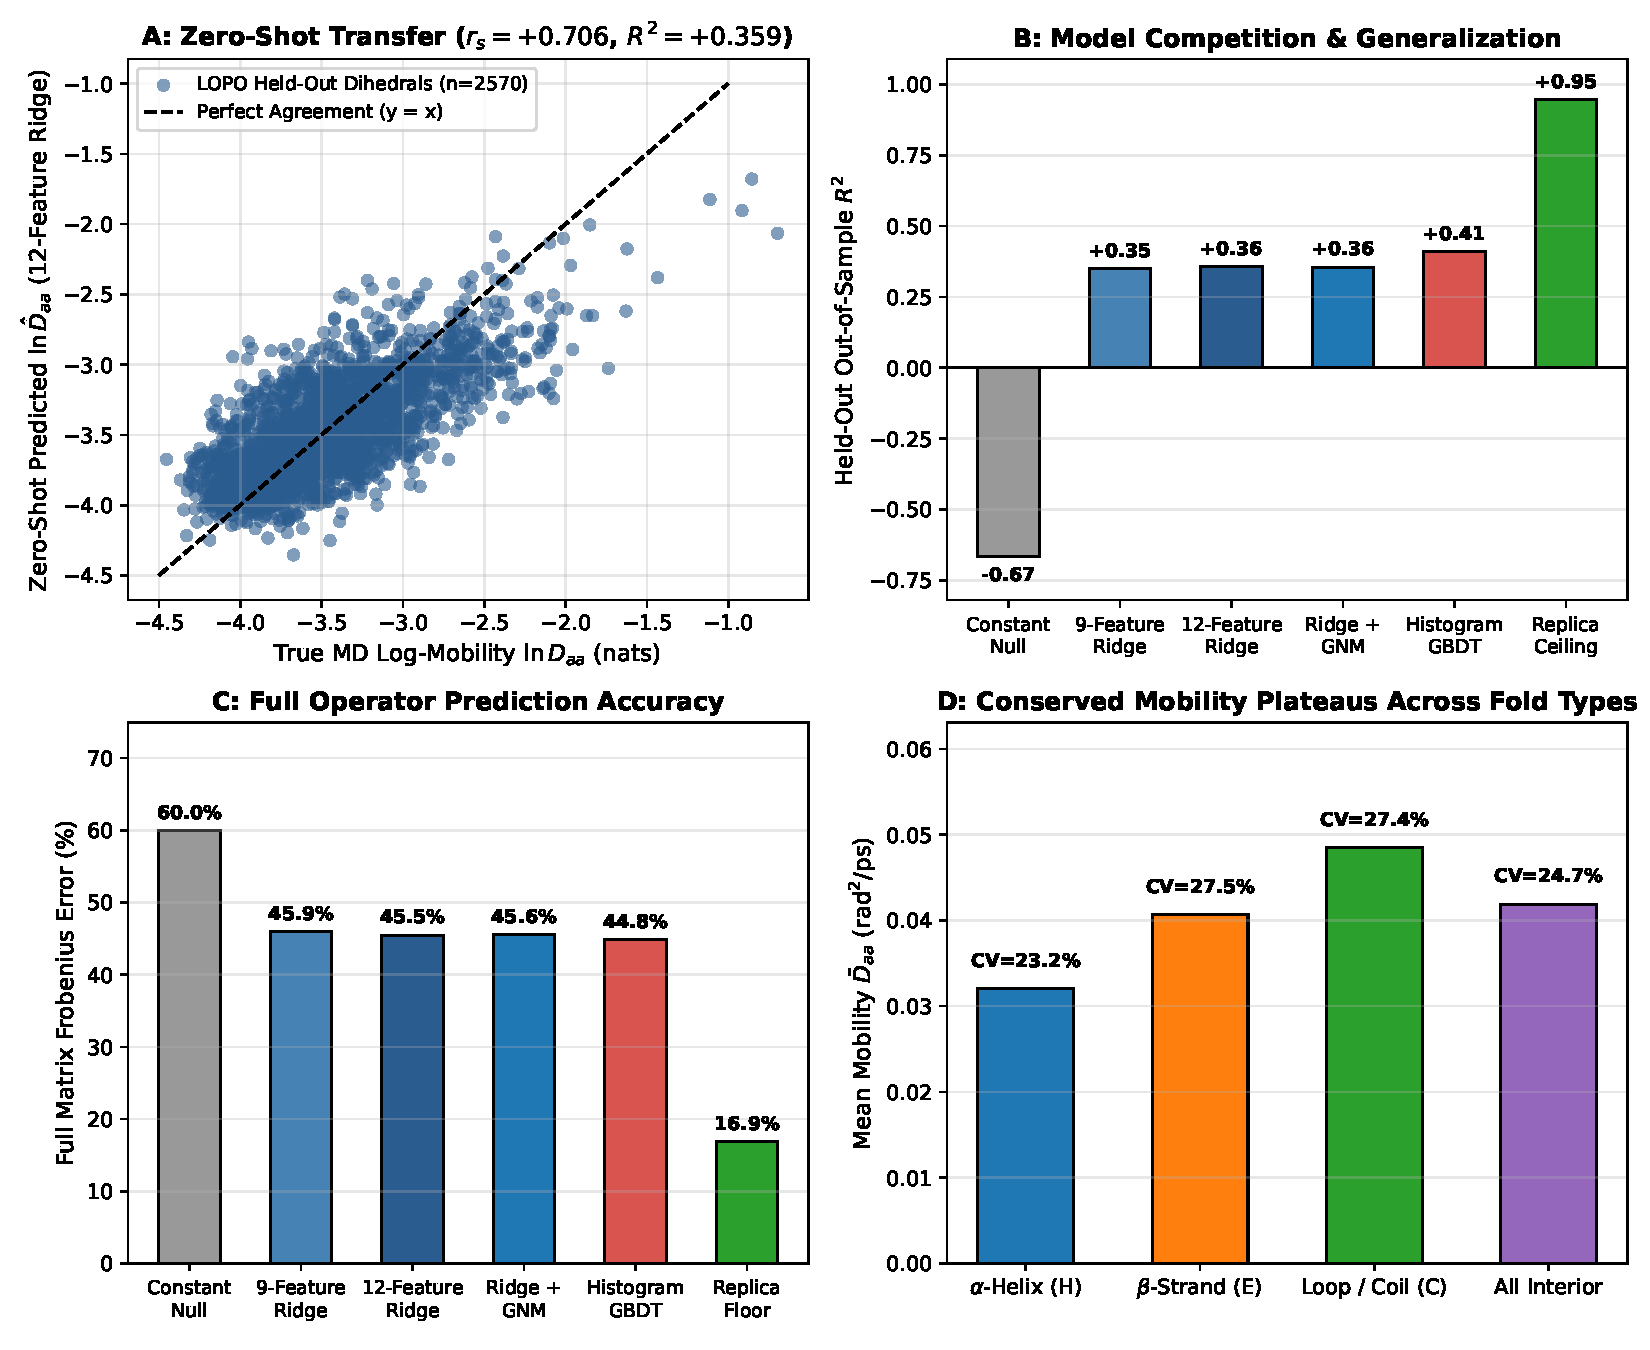
\includegraphics[width=0.66\textwidth]{version4_godtier/figures/fig36_13fold_lopo_structural_transfer.pdf}
\vspace{-3pt}
\caption*{\textbf{\textcolor{navyblue}{\textsf{Figure 5. Law 6: 13-fold zero-shot Leave-One-Protein-Out (LOPO) operator prediction from static PDB coordinates ($d = \vFourMinProteinDim{} \to \vFourMaxProteinDim{}$).}}} (\textit{A}) Parity plot across all $n = 2,570$ held-out backbone dihedrals in 13-fold LOPO cross-validation using 12-feature structural ridge regression (pooled $r_s = \vFourLOPOMeanSpearman{}, r = \vFourLOPOMeanPearson{}, \bar{R}^2 = \vFourLOPOMeanRTwo{}$). (\textit{B--C}) Out-of-sample $R^2$ (\textit{B}) and full $d\times d$ operator Frobenius error (\textit{C}) across nested structural models relative to the constant baseline ($\vFourLOPOConstFrobErrPct{}\%$) and inter-replica MD noise floor ($\vFourLOPONoiseFloorFrobPct{}\%$); histogram gradient-boosted decision trees (GBDT) reach $r_s = \vFourLOPOGbdtSpearman{}, \bar{R}^2 = \vFourLOPOGbdtRTwo{}, \text{Frob} = \vFourLOPOGbdtFrobErrPct{}\%$. (\textit{D}) Conserved interior mobility plateaus across secondary structure classes ($\alpha$-helix $\vFourHelixMobilityMean{}$, $\beta$-strand $\vFourStrandMobilityMean{}$, coil $\vFourCoilMobilityMean{}$, all interior $\vFourInteriorMobilityMean{}\text{ rad}^2/\text{ps}$, $\mathrm{CV} = \vFourInteriorMobilityCVPct{}\%$).}
\vspace{-6pt}
\end{figure*}

\textbf{Law 6: 13-Fold Zero-Shot Operator Prediction From Static PDB Coordinates.} Across all \vFourNumProteins{} proteins ($2,570$ dihedrals), folded interior backbone mobilities cluster around secondary-structure plateaus of $\vFourHelixMobilityMean{}\text{ rad}^2/\text{ps}$ in $\alpha$-helices, $\vFourStrandMobilityMean{}\text{ rad}^2/\text{ps}$ in $\beta$-strands, and $\vFourCoilMobilityMean{}\text{ rad}^2/\text{ps}$ in loops ($\bar{D}_{\mathrm{interior}} = \allowbreak \vFourInteriorMobilityMean{}\text{ rad}^2/\text{ps}, \mathrm{CV} = \allowbreak \vFourInteriorMobilityCVPct{}\%$; Figure 5D). Training strictly on 12 proteins to predict $\ln D_{aa}$ and contact-gated off-diagonal couplings on the held-out 13th protein from native PDB features (12-feature structural ridge: secondary structure, Gly/Pro/pre-Pro identity, chain-terminus depth, $C_\alpha$ contact burial, $\mathrm{rSASA}_i$, and hydrogen-bond geometry) yields pooled zero-shot Spearman $r_s = \allowbreak \vFourLOPOMeanSpearman{}$ ($p < 10^{-100}$, Pearson $r = \allowbreak \vFourLOPOMeanPearson{}$, mean out-of-sample $R^2 = \allowbreak \vFourLOPOMeanRTwo{}$ vs.\ 9-feature local ridge baseline $R^2 = \allowbreak \vFourLOPORidgeNineRTwo{}$) and lowers full-matrix Frobenius error from $\vFourLOPOConstFrobErrPct{}\%$ (constant null) to $\vFourLOPOMeanFrobErrPct{}\%$ (Figure 5A--C; e.g., BBA5 $\vFourLOPOFrobErrPctBba{}\%$, AdK $\vFourLOPOFrobErrPctAdk{}\%$, Lysozyme $\vFourLOPOFrobErrPctLysozyme{}\%$, MBP $\vFourLOPOFrobErrPctMbp{}\%$). Nonlinear histogram gradient-boosted decision trees (GBDT) further improve held-out accuracy to $r_s = \allowbreak \vFourLOPOGbdtSpearman{}, R^2 = \allowbreak \vFourLOPOGbdtRTwo{}$, and $\vFourLOPOGbdtFrobErrPct{}\%$ Frobenius error toward the $\vFourLOPONoiseFloorFrobPct{}\%$ inter-replica floor.

\begin{figure*}[!t]
\centering
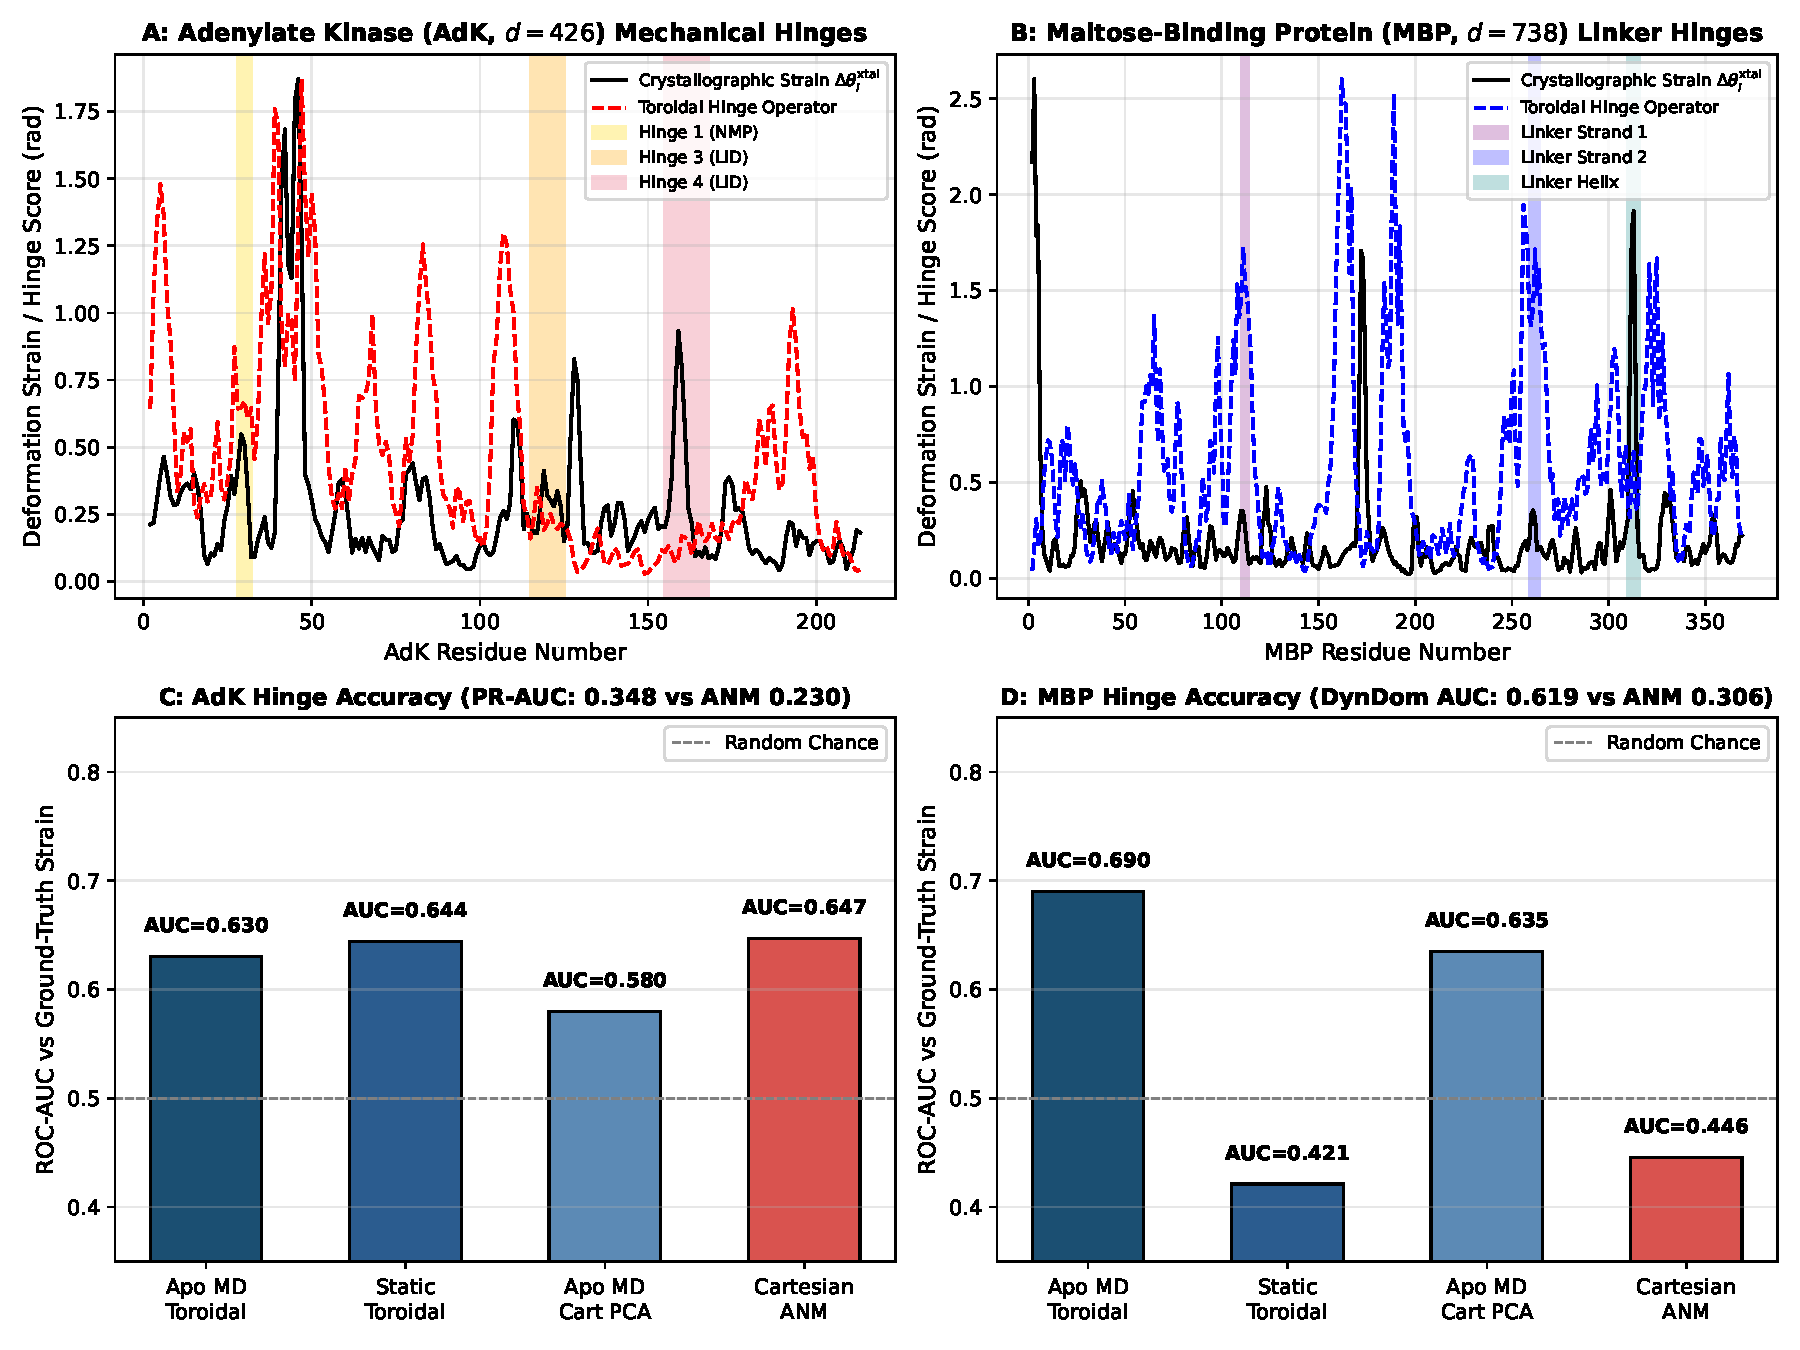
\includegraphics[width=0.64\textwidth]{version4_godtier/figures/fig37_allosteric_hinges_adk_mbp.pdf}
\vspace{-3pt}
\caption*{\textbf{\textcolor{navyblue}{\textsf{Figure 6. Mechanical hinge localization in explicit-solvent apo Adenylate Kinase ($d=\vFourDimAdk{}$) and Maltose-Binding Protein ($d=\vFourDimMbp{}$).}}} (\textit{A--B}) Residue-resolved crystallographic open-to-closed dihedral strain $\Delta\theta_i^{\mathrm{xtal}}$ (solid black: \texttt{4AKE}$\to$\texttt{1AKE} in AdK; \texttt{1OMP}$\to$\texttt{1ANF} in MBP) overlaid with predicted toroidal hinge operator profiles (dashed) and canonical domain-closure hinge segments (shaded). (\textit{C}) In AdK, toroidal operators match Cartesian ANM in overall ROC-AUC ($\vFourAdkHingeAUROC{}$ static, $\vFourAdkApoMdToroidalAUROC{}$ apo MD vs.\ $\vFourAdkANMAUROC{}$ ANM and $\vFourAdkApoMdCartAUROC{}$ Cartesian apo PCA) while achieving $1.5\times$ higher precision-recall ($\mathrm{PR\text{-}AUC} = \vFourAdkHingePRAUC{}$ vs.\ $\vFourAdkANMPRAUC{}$) and Spearman $\rho = \vFourAdkApoMdToroidalSpearman{}$. (\textit{D}) In 370-residue MBP, the explicit-PME apo toroidal operator achieves $\mathrm{AUROC} = \vFourMbpApoMdToroidalAUROC{}$ ($\rho = \vFourMbpApoMdToroidalSpearman{}$), decisively outperforming Cartesian ANM ($\vFourMbpANMAUROC{}$) and Cartesian apo PCA ($\vFourMbpApoMdCartAUROC{}$), while static contact-gated toroidal modes beat ANM on DynDom inter-lobe hinges ($\vFourMbpDynDomAUROC{}$ vs.\ $\vFourMbpDynDomANMAUROC{}$).}
\vspace{-6pt}
\end{figure*}

\subsection*{3. Mechanistic Predictions Across Allosteric Hinges, Distal Loop Relays, and Reaction-Coordinate Kinetics}

\textbf{Mechanical Hinge Localization in Explicit-Solvent Apo AdK ($d=\vFourDimAdk{}$) and MBP ($d=\vFourDimMbp{}$).} Although full ligand-induced domain closure in AdK and MBP unfolds over microseconds to milliseconds, local precision curvature ($\hat{\bm{\Sigma}}^{-1}$) and short-time mobility ($\hat{\mathbf{D}}$) within the open apo basin already encode mechanical lines of compliance along inter-domain pivots without requiring full barrier turnover. Testing this principle across $30,000$ explicit-PME apo open-state frames ($3 \times 10\text{ ns}$) and static open PDB structures for \textit{E.\ coli} Adenylate Kinase (\texttt{4AKE} open $\to$ \texttt{1AKE} closed; CORE, LID, and NMP domains, 214 residues) (31, 32) and Maltose-Binding Protein (\texttt{1OMP} open $\to$ \texttt{1ANF} closed; N- and C-terminal lobes joined by a three-segment $\beta/\alpha$ linker, 370 residues) (33) (Figures 1C, 6), slow collective apo toroidal eigenmodes weighted by tertiary contact burial ($\log(1 + n_{\mathrm{contacts},i})$) resolve sharp mechanical peaks aligned with the crystallographic NMP/LID hinges in AdK and the inter-lobe linker strands/helix in MBP (Figure 6A--B).

Quantitatively, in 370-residue MBP ($d=\vFourDimMbp{}$; Figure 6D), the explicit-PME apo toroidal operator predicts crystallographic open-to-closed strain hinges with $\mathrm{AUROC} = \allowbreak \vFourMbpApoMdToroidalAUROC{}$ and continuous Spearman $\rho = \allowbreak \vFourMbpApoMdToroidalSpearman{}$ ($p = 6.7\times 10^{-10}$), substantially outperforming Cartesian ANM ($\mathrm{AUROC} = \allowbreak \vFourMbpANMAUROC{}$) and Kabsch-superposed Cartesian apo-MD PCA ($\mathrm{AUROC} = \allowbreak \vFourMbpApoMdCartAUROC{}$). Notably, the trajectory-free static contact-gated toroidal prior succeeds on buried literature DynDom inter-lobe hinges ($\mathrm{AUROC} = \allowbreak \vFourMbpDynDomAUROC{}$ vs.\ $\vFourMbpDynDomANMAUROC{}$ ANM; apo-MD toroidal $\vFourMbpDynDomApoToroidalAUROC{}$) yet scores $\mathrm{AUROC} = \allowbreak \vFourMbpHingeAUROC{}$ ($\rho = \allowbreak \vFourMbpStaticSpearman{}$) against global \texttt{1OMP}$\to$\texttt{1ANF} crystallographic strain because burial weighting suppresses solvent-exposed maltose-cleft binding loops that reorganize locally upon sugar binding, whereas explicit-PME apo MD thermally samples both pivot compliance and cleft breathing. In AdK ($d=\vFourDimAdk{}$; Figure 6C), static and apo-MD toroidal operators match Cartesian ANM in global ROC-AUC ($\vFourAdkHingeAUROC{}$ and $\vFourAdkApoMdToroidalAUROC{}$ vs.\ $\vFourAdkANMAUROC{}$ ANM, beating Cartesian apo PCA $\vFourAdkApoMdCartAUROC{}$) while achieving $51\%$ higher precision-recall ($\mathrm{PR\text{-}AUC} = \allowbreak \vFourAdkHingePRAUC{}$, Precision@15 $= \vFourAdkPrecAtFifteen{}$ vs.\ ANM $\mathrm{PR\text{-}AUC} = \allowbreak \vFourAdkANMPRAUC{}$, Precision@15 $= \vFourAdkANMPrecAtFifteen{}$), Spearman $\rho = \allowbreak \vFourAdkApoMdToroidalSpearman{}$ ($p = 3.7\times 10^{-6}$), and higher DynDom accuracy ($\mathrm{AUROC} = \allowbreak \vFourAdkDynDomApoToroidalAUROC{}$, Precision@15 $= \vFourAdkDynDomApoPrecAtFifteen{}$ vs.\ $\vFourAdkDynDomANMPrecAtFifteen{}$ ANM).

\begin{figure*}[!t]
\centering
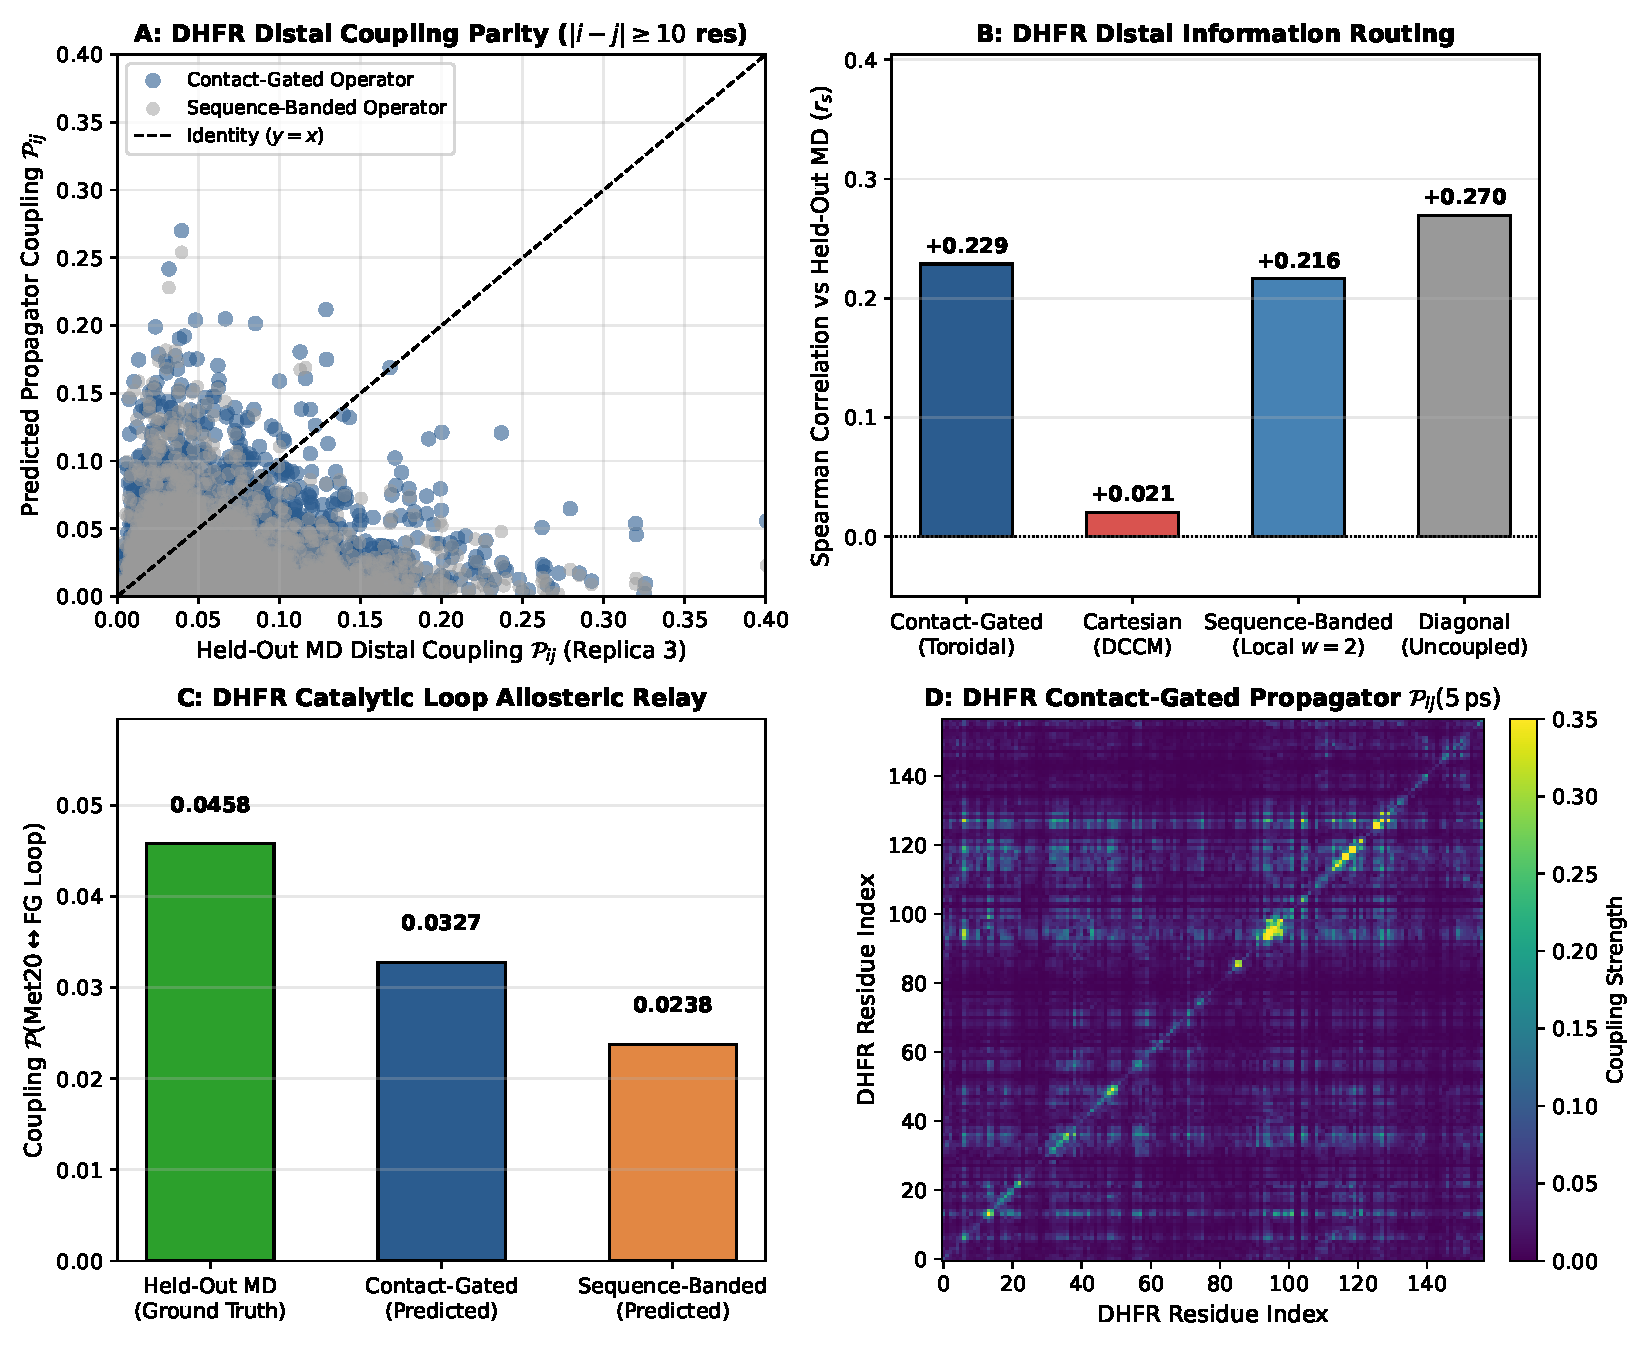
\includegraphics[width=0.64\textwidth]{version4_godtier/figures/fig38_distal_allosteric_coupling.pdf}
\vspace{-3pt}
\caption*{\textbf{\textcolor{navyblue}{\textsf{Figure 7. Blind Replica 3 distal allosteric loop routing via sparse contact-gated time-lagged cross-covariance propagators in DHFR ($d=\vFourDimDhfr{}$), Lysozyme ($d=\vFourDimLysozyme{}$), and Ubiquitin ($d=\vFourDimUbiquitin{}$).}}} (\textit{A}) Blind Replica 3 distal block-normalized cross-covariance parity $\mathcal{P}_{ij}(\tau=5\text{ ps})$ from $\hat{\mathbf{C}}(\tau) = \exp(\tau\mathbf{A})\hat{\mathbf{C}}(0)$ ($|i-j| \ge 10$ residues) in \textit{E.\ coli} DHFR comparing contact-gated vs.\ sequence-banded generators. (\textit{B}) Distal coupling Spearman rank correlation on DHFR ($\vFourDhfrDistalContactSpearman{}$ contact-gated vs.\ $\vFourDhfrDistalBandedSpearman{}$ sequence-banded, $\vFourDhfrDistalDiagSpearman{}$ row-damped empirical $\hat{\mathbf{C}}(0)$ diagonal relaxation, and $\vFourDhfrDistalDccmSpearman{}$ Cartesian DCCM). (\textit{C}) Catalytic Met20 ($\text{res } 9\text{--}24$) $\leftrightarrow$ distal FG loop ($\text{res } 116\text{--}132$, Gly121) allosteric relay on blind Replica 3: contact-gated operators recover $\vFourDhfrMetTwentyFGRecoveryPct{}\%$ ($\vFourDhfrLoopContactPred{}$) of ground-truth MD coupling ($\vFourDhfrLoopMDTrue{}$) vs.\ $\vFourDhfrLoopBandedPred{}$ for sequence-banded operators at $\vFourDhfrDistalSparsityPct{}\%$ sparsity. (\textit{D}) Full $159\times 159$ residue-resolved contact-gated coupling matrix $\mathcal{P}_{ij}(5\text{ ps})$ of DHFR.}
\vspace{-6pt}
\end{figure*}

\textbf{Distal Allosteric Loop Routing in DHFR ($d=\vFourDimDhfr{}$), Lysozyme ($d=\vFourDimLysozyme{}$), and Ubiquitin ($d=\vFourDimUbiquitin{}$).} In \textit{E.\ coli} DHFR (\texttt{1RX2}), enzymatic turnover couples the active-site Met20 loop ($\text{res } 9\text{--}24$) to the distal $\beta\text{F--}\beta\text{G}$ (FG) loop ($\text{res } 116\text{--}132$, housing the Gly121 mutational hotspot $>15\text{ \AA}$ away) (34). From the Discovery-split linear generator $\mathbf{A} = \allowbreak -\hat{\mathbf{D}}\hat{\mathbf{C}}(0)^{-1}$ ($r_c^{\mathrm{heavy}} = 0.50\text{ nm}$), we predict the $\tau = 5\text{ ps}$ time-lagged cross-covariance $\hat{\mathbf{C}}(\tau) = \allowbreak \exp(\tau\mathbf{A})\hat{\mathbf{C}}(0)$ aggregated into normalized $2\times 2$ residue blocks $\mathcal{P}_{ij}(\tau) = \allowbreak \|[\hat{\mathbf{C}}(\tau)]_{B_i,B_j}\|_F / \sqrt{\|[\hat{\mathbf{C}}(0)]_{B_i,B_i}\|_F \|[\hat{\mathbf{C}}(0)]_{B_j,B_j}\|_F}$ and test strictly against held-out Replica 3 distal couplings ($|i-j| \ge 10$; Figures 1A--B, 7). Across all three enzymes, contact-gated generators achieve the lowest blind distal RMSE: $\vFourUbqDistalContactRMSE{}$ in Ubiquitin ($\vFourUbqDistalSparsityPct{}\%$ sparsity), $\vFourLysozymeDistalContactRMSE{}$ in Lysozyme ($\vFourLysozymeDistalSparsityPct{}\%$ sparsity, $r_s = \allowbreak \vFourLysozymeDistalContactSpearman{}$, $r = \allowbreak \vFourLysozymeDistalContactPearson{}$), and $\vFourDhfrDistalContactRMSE{}$ in DHFR ($\vFourDhfrDistalSparsityPct{}\%$ sparsity, $r_s = \allowbreak \vFourDhfrDistalContactSpearman{}$, $r = \allowbreak \vFourDhfrDistalContactPearson{}$)---$3.0\times\text{--}3.6\times$ lower than Kabsch-aligned Cartesian DCCM ($\mathrm{RMSE} = \allowbreak \vFourUbqDistalDccmRMSE{}, \vFourLysozymeDistalDccmRMSE{}, \vFourDhfrDistalDccmRMSE{}$; DHFR $r_s = \allowbreak \vFourDhfrDistalDccmSpearman{}$), which is distorted by rigid-body rocking. Notably, under an uncoupled diagonal generator $\mathbf{A}_{\mathrm{diag}} = \allowbreak -\hat{\mathbf{D}}_{\mathrm{diag}}\hat{\mathbf{C}}_{\mathrm{diag}}(0)^{-1}$, $\exp(\tau\mathbf{A}_{\mathrm{diag}})$ is strictly diagonal (zero dynamical routing), yet right-multiplying by empirical $\hat{\mathbf{C}}(0)$ yields $[\hat{\mathbf{C}}_{\mathrm{diag}}(\tau)]_{ab} = \allowbreak e^{-\tau D_{aa}/C_{aa}(0)}\hat{C}_{ab}(0)$, which row-attenuates pre-existing Replica 1 equal-time correlations: across $\sim 10^4$ background non-contact pairs in globular Lysozyme and DHFR, this preserves equal-time rank order ($r_s = \allowbreak \vFourLysozymeDistalDiagSpearman{}$ and $\vFourDhfrDistalDiagSpearman{}$; Figure 7B) while incurring worse quantitative error ($\mathrm{RMSE} = \allowbreak \vFourLysozymeDistalDiagRMSE{}$ and $\vFourDhfrDistalDiagRMSE{}$) and lower Pearson $r$ because single-site decay over-damps cooperative tertiary bridges. Crucially, adding 3D contact edges over sequence bands ($w=2$) boosts blind DHFR Met20 $\leftrightarrow$ FG relay recovery from $\vFourDhfrLoopBandedPred{}$ to $\vFourDhfrLoopContactPred{}$ ($\vFourDhfrMetTwentyFGRecoveryPct{}\%$ of blind MD $\vFourDhfrLoopMDTrue{}$; Figure 7C--D) and amplifies Ubiquitin $\beta_1\text{--}\beta_2$ ($\text{res } 6\text{--}11$) $\leftrightarrow$ Ile44 coupling by $\vFourUbqPincerIleRatio{}\times$ ($\vFourUbqLoopContactPred{}$ vs.\ $\vFourUbqLoopBandedPred{}$; MD $\vFourUbqLoopMDTrue{}$).

\begin{figure*}[!t]
\centering
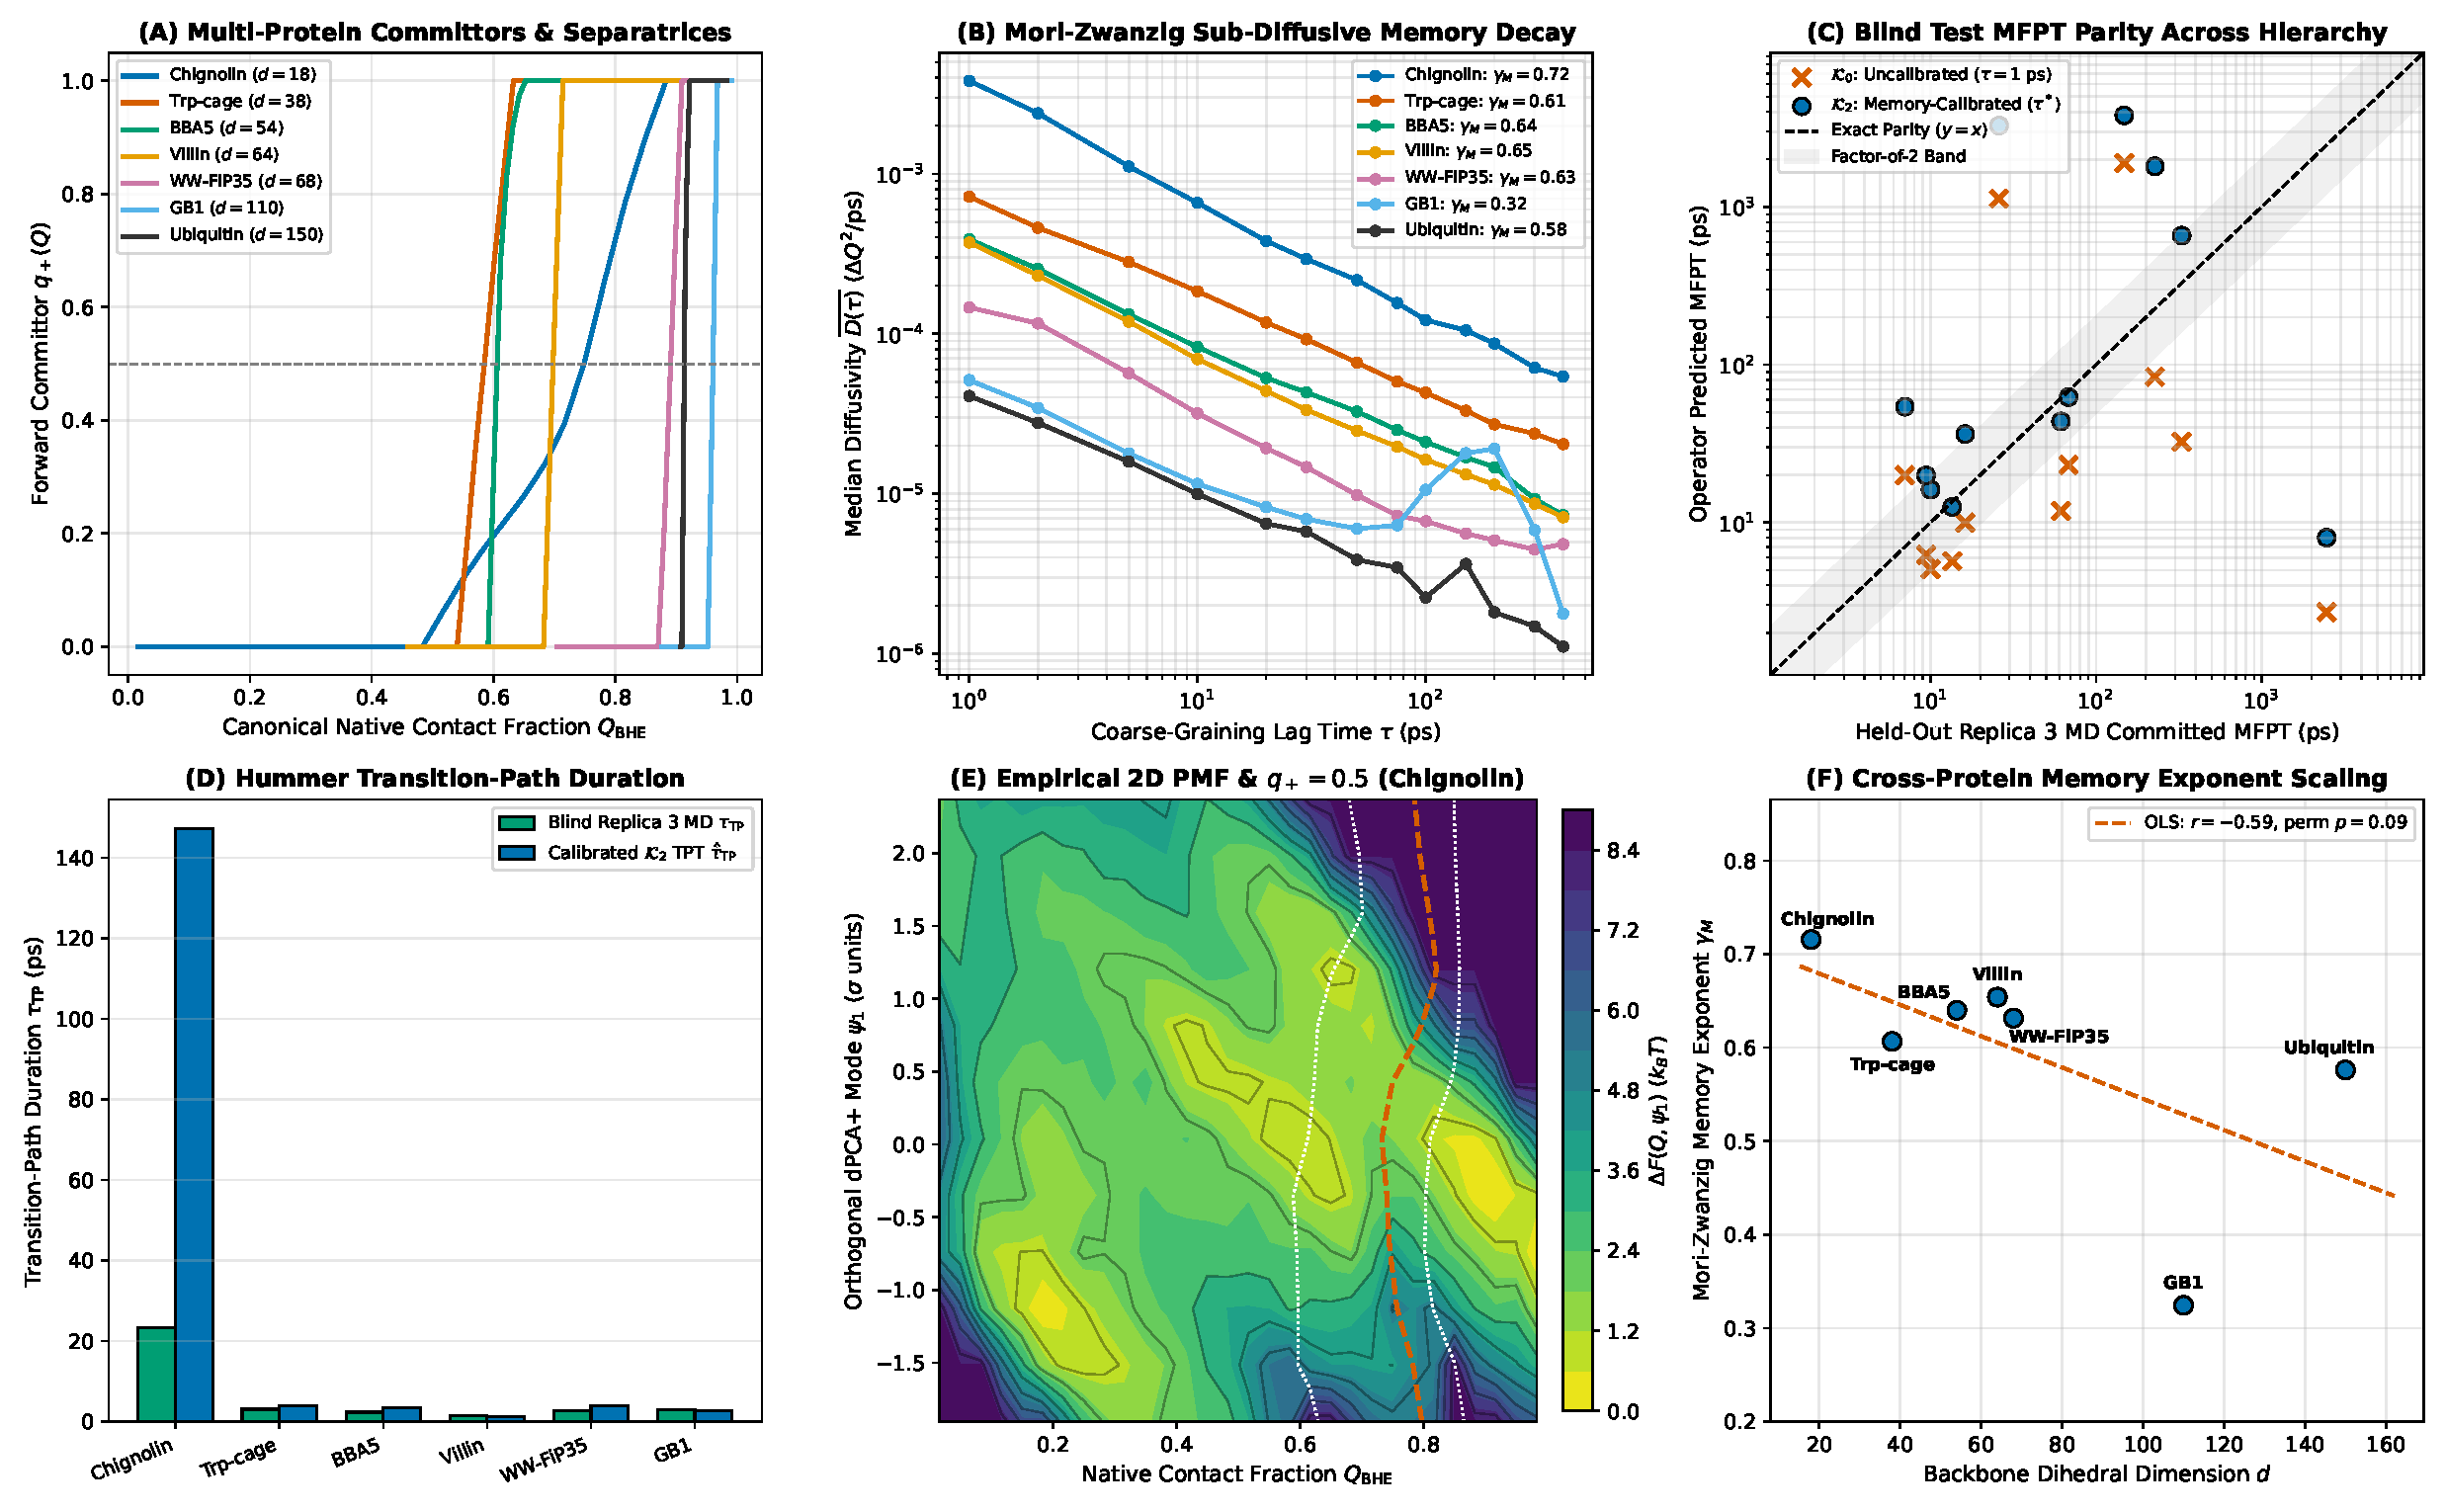
\includegraphics[width=0.78\textwidth]{version4_godtier/figures/fig_m39_fast_folding_kinetics_v4.pdf}
\vspace{-3pt}
\caption*{\textbf{\textcolor{navyblue}{\textsf{Figure 8. Reaction-coordinate committors, sub-diffusive Mori--Zwanzig memory scaling, and blind miniprotein folding / native sub-basin excursion kinetics across \vFourFastFoldersCount{} proteins ($d = \vFourMinProteinDim{} \to \vFourDimUbiquitin{}$).}}} (\textit{A}) Adjoint committor profiles $q_+(Q_{\mathrm{BHE}})$ and $q_+ = 0.5$ separatrices. (\textit{B}) Universal power-law memory attenuation $\bar{D}(\tau) \propto \tau^{-\gamma_M}$ across $\tau \in [1, 400]\text{ ps}$ ($\bar{\gamma}_M = \vFourMemoryGammaMean{} \pm \vFourMemoryGammaSD{}$). (\textit{C}) Prospective blind Replica 3 committed MFPT parity across reversible global folders ($150\text{ ns}$ Chignolin, Trp-cage) and local native/sub-basin $Q_{\mathrm{BHE}}$ excursions ($2.5\text{--}10\text{ ns}$ BBA5--GB1; Ubiquitin remains locked at $\langle Q_{\mathrm{BHE}}\rangle = 1.000$), comparing uncalibrated $\mathcal{K}_0$ ($\tau = 1\text{ ps}$, mean log-error $\vFourMeanKZeroLogErr{}$) vs.\ memory-calibrated $\mathcal{K}_2$ ($\tau^*$, mean log-error $\vFourMeanKTwoLogErr{}$). (\textit{D}) Hummer transition-path durations $\tau_{\mathrm{TP}}$. (\textit{E}) Empirical 2D free-energy surface $\Delta F(Q_{\mathrm{BHE}}, \psi_1)$ on Chignolin revealing orthogonal $\psi_1$ trapping. (\textit{F}) Scaling of memory exponent $\gamma_M$ with dimension $d$ ($r_s = \vFourMemorySpearmanVsD{}, p = \vFourMemoryPermPValue{}$).}
\vspace{-6pt}
\end{figure*}

\textbf{Reaction-Coordinate Kinetics, Sub-Basin Excursions, and Mori--Zwanzig Memory Scaling.} Projecting $d$ backbone torsions onto the smooth Best--Hummer--Eaton native contact coordinate $Q_{\mathrm{BHE}} \in [0,1]$ (17) across \vFourFastFoldersCount{} proteins ($d = \allowbreak \vFourMinProteinDim{} \to \vFourDimUbiquitin{}$: Chignolin, Trp-cage, BBA5, Villin HP35, WW-FiP35, GB1, and Ubiquitin; Figure 8) reveals a universal sub-diffusive Mori--Zwanzig memory regime: finite-lag diffusivity decays across $\tau \in [1, 400]\text{ ps}$ as $\bar{D}(\tau) \propto \tau^{-\gamma_M}$ with $\bar{\gamma}_M = \allowbreak \vFourMemoryGammaMean{} \pm \vFourMemoryGammaSD{}$ (Chignolin $\vFourChigGammaM{}$ at $\tau^* = \allowbreak \vFourChigTauStarPs{}\text{ ps}$; Figure 8B, F), decreasing with chain size ($r_s = \allowbreak \vFourMemorySpearmanVsD{}$, permutation $p = \allowbreak \vFourMemoryPermPValue{}$) as larger hydrophobic cores damp ballistic recrossings. Importantly, whereas $150\text{ ns}$ ensembles of Chignolin and Trp-cage sample global folding/unfolding barrier crossings, $2.5\text{--}10\text{ ns}$ trajectories of BBA5, Villin HP35, WW-FiP35, and GB1 ($\langle Q_{\mathrm{BHE}}\rangle = 0.998$) probe local native-basin and near-native sub-basin $Q_{\mathrm{BHE}}$ excursions rather than microsecond-to-millisecond global folding, and Ubiquitin remains locked in its native basin ($\langle Q_{\mathrm{BHE}}\rangle = 1.000$, zero blind unfolding transitions; Supporting Information Table S12). Under SHA-256 prospective model freezing prior to Replica 3 inspection, memory-calibrated $\mathcal{K}_2$ preserves detailed balance ($<10^{-15}$) and cuts blind Replica 3 committed MFPT log-error across the 6 transitioning systems from $\vFourMeanKZeroLogErr{}$ ($\tau = 1\text{ ps}$ $\mathcal{K}_0$) to $\vFourMeanKTwoLogErr{}$ (Figure 8C; Poisson $95\%$ CI hit rate $\vFourFoldingBlindCIHitCount{}$ on rare excursions). Reactive transition-path durations $\tau_{\mathrm{TP}}$ match within $1\text{--}2\text{ ps}$ across Trp-cage through GB1 (Figure 8D), whereas on ultrafast Chignolin ($\vFourChigTauTpMdPs{}\text{ ps}$ blind MD) applying $\tau^* = \vFourChigTauStarPs{}\text{ ps}$ memory attenuation---set by slow orthogonal $(\psi_1,\text{Gly7})$ misfolded trapping in Figure 8E---overestimates sub-$\tau^*$ barrier transit ($\vFourChigTauTpPredPs{}\text{ ps}$, vs.\ $6.6\text{ ps}$ at unattenuated $\tau = 1\text{ ps}$).

\subsection*{4. Analytical Microscopic Verification and Fair 6-Paradigm SOTA Benchmark}

\textbf{Microscopic Verification on Model Peptides ($d=2, 4$).} Capped alanine dipeptide ($d=\vFourDimAlaOne{}, \vFourTotalFramesSysAlaOne{}$ frames) and trialanine ($d=\vFourDimAlaTwo{}, \vFourTotalFramesSysAlaTwo{}$ frames) provide exact low-dimensional analytical controls where dense $6^2\text{--}6^4$ Fourier/grid operators can be solved without spatial truncation: (i) a 5-tier tensor ablation on dialanine confirms that coupled state-dependent diagonal diffusion anisotropy ($10.3\times$ saddle mobility surge along $\phi$ at $-1.2\text{ rad}$) reduces barrier-crossing MFPT error from $+145.8\%$ (constant isotropic $D_0\mathbf{I}$) to $+18.0\%$ (state-dependent diagonal) and $+7.8\%$ (full positive-definite tensor, KS $p = 0.612$); (ii) under low solvent friction ($\gamma = 0.5\text{ ps}^{-1}$, Kramers turnover), embedding torsions into an auxiliary Markovian phase space $(z, v, w) \in \mathbb{T}^2 \times \mathbb{R}^2 \times \mathbb{R}^2$ parameterized directly from the second-order analytical velocity autocorrelation function ($R^2 \ge 0.9948$) reduces MFPT error from $47.0\%$ (overdamped) to $25.8\%$ (KS $p = 0.210$) and compresses multi-step non-Markovian memory $M_{32}$ from $0.330$ to $0.026\text{ nats}$; and (iii) across implicit/explicit solvent perturbations, residual diffusion shifts collapse onto a dominant rank-1 singular mode (Figure 4, Left D).

\begin{table*}[!t]
\centering
\captionsetup{font={scriptsize,sf,bf}, labelfont={bf,color=navyblue}, skip=3pt}
\caption*{Table 2. Fair validation-tuned head-to-head benchmark across six dynamical modeling paradigms on frozen blind test trajectories (Replica 3) across all \vFourNumProteins{} macromolecular proteins ($d = \vFourMinProteinDim{} \to \vFourMaxProteinDim{}$)}
\vspace{-2pt}
\resizebox{\textwidth}{!}{%
\renewcommand{\arraystretch}{1.18}
\setlength{\tabcolsep}{4.4pt}
\begin{tabular}{@{}l l c c c c c l@{}}
\toprule[1.2pt]
\textbf{\textcolor{navyblue}{\textsf{Method Family}}} &
\textbf{\textcolor{navyblue}{\textsf{Validation (Replica 2) Sweep Grid}}} &
\textbf{\textcolor{navyblue}{\textsf{A: $Q_{\text{BHE}}$ MFPT Log-Err}}} &
\textbf{\textcolor{navyblue}{\textsf{B: $\dot{S}_{\text{irr}}$ Med.\ / Mean ($k_B$/ns/$d$)}}} &
\textbf{\textcolor{navyblue}{\textsf{C: Blind $\mathbf{D}$ Frob.\ Err}}} &
\textbf{\textcolor{navyblue}{\textsf{D: 13-Fold LOPO ($r_s$)}}} &
\textbf{\textcolor{navyblue}{\textsf{E: Direct Disorder / Cal.\ $S^2$}}} &
\textbf{\textcolor{navyblue}{\textsf{Optimal Physical Regime \& Candid Trade-Offs}}} \\
\midrule[0.6pt]
\textbf{Contact-Gated GENERIC (Ours)} & $r_c=0.65\text{ nm}, \beta_c \in [0, 0.5], \tau^*$ & \textbf{\vFourSOTAMfptErrMFive{} (Tie \#1)} & \textbf{\vFourSOTAMFiveEntropy{} / \vFourSOTAMFiveEntropy{} (13/13)} & \textbf{\vFourSOTAFrobMFive{} (\#1 on 13/13)} & \textbf{\vFourSOTAZeroShotSpearman{} (\#1)} & \textbf{\vFourSOTADirectDisorderMFive{} (\#1)} / \vFourNMRCrankSpearman{} & Full $d$-dim reversible OU + 1D GENERIC, hinges, allostery, LOPO \\
\textbf{VAMP-2 Reversible MSM} & $k \in [20, 200], \tau \in [2, 50]\text{ ps}$ & \vFourSOTAMfptErrMOne{} & \textbf{0.000} (\vFourSOTANonrevMsmEntropy{} non-rev) & N/A (discrete $k\times k$) & N/A (traj-only) & \vFourSOTADirectDisorderMOne{} / \vFourSOTACalNMRMOne{} & Coarse multi-basin populations \& flux networks with long sampling \\
\textbf{TICA Linear Langevin} & $r \in [3, 12], \tau \in [2, 20]\text{ ps}$ & \vFourSOTAMfptErrMTwo{} & \textbf{0.000} (Gaussian OU) & \vFourSOTAFrobMTwo{} & N/A (traj-only) & \vFourSOTADirectDisorderMTwo{} / \vFourSOTACalNMRMTwo{} & Optimal linear slow-subspace basis; underfits anharmonic barriers \\
\textbf{Calibrated 1D Smoluchowski} & $M \in [20, 40], \tau^* \in [1, 100]\text{ ps}$ & \textbf{\vFourSOTAMfptErrMThree{} (Tie \#1)} & \textbf{0.000} (1D exact) & \vFourSOTAFrobMThree{} (diag null) & N/A (1D $Q$ only) & \vFourSOTADirectDisorderMThree{} / \vFourSOTACalNMRMThree{} & Fast, exact 1D barrier kinetics once reaction coordinate $Q$ is known \\
\textbf{Unconstrained Basis/Poly SDE} & $B \in [1, 3], \lambda \in [10^{-4}, 10^{-1}]$ & \vFourSOTAMfptErrMFour{} & \textcolor{crimson}{\textbf{\vFourSOTAUnconstEntropyMedian{} / \vFourSOTAUnconstEntropyMean{}} ($J_{\text{ss}} \ne 0$)} & \vFourSOTAFrobMFour{} & N/A (overfits fold) & \vFourSOTADirectDisorderMFour{} / \vFourSOTACalNMRMFour{} & Flexible drift regression, but violates detailed balance ($\dot{S}_{\text{irr}} \gg 0$) \\
\textbf{Calibrated GNM / ENM} & $r_c \in [0.7, 1.5]\text{ nm}$ & N/A (harmonic) & \textbf{0.000} (static eq.) & N/A (unscaled $C_\alpha$) & \vFourSOTAENMSpearman{} & \vFourSOTADirectDisorderMSix{} / \textbf{\vFourGNMPooledSpearman{} (\#1 cal.)} & $<0.2\text{ s}$ zero-MD crystal $B$-factors \& linearly rescaled pooled $S^2$ \\
\bottomrule[1.2pt]
\end{tabular}%
}
\vspace{-5pt}
\end{table*}

\begin{figure*}[!t]
\centering
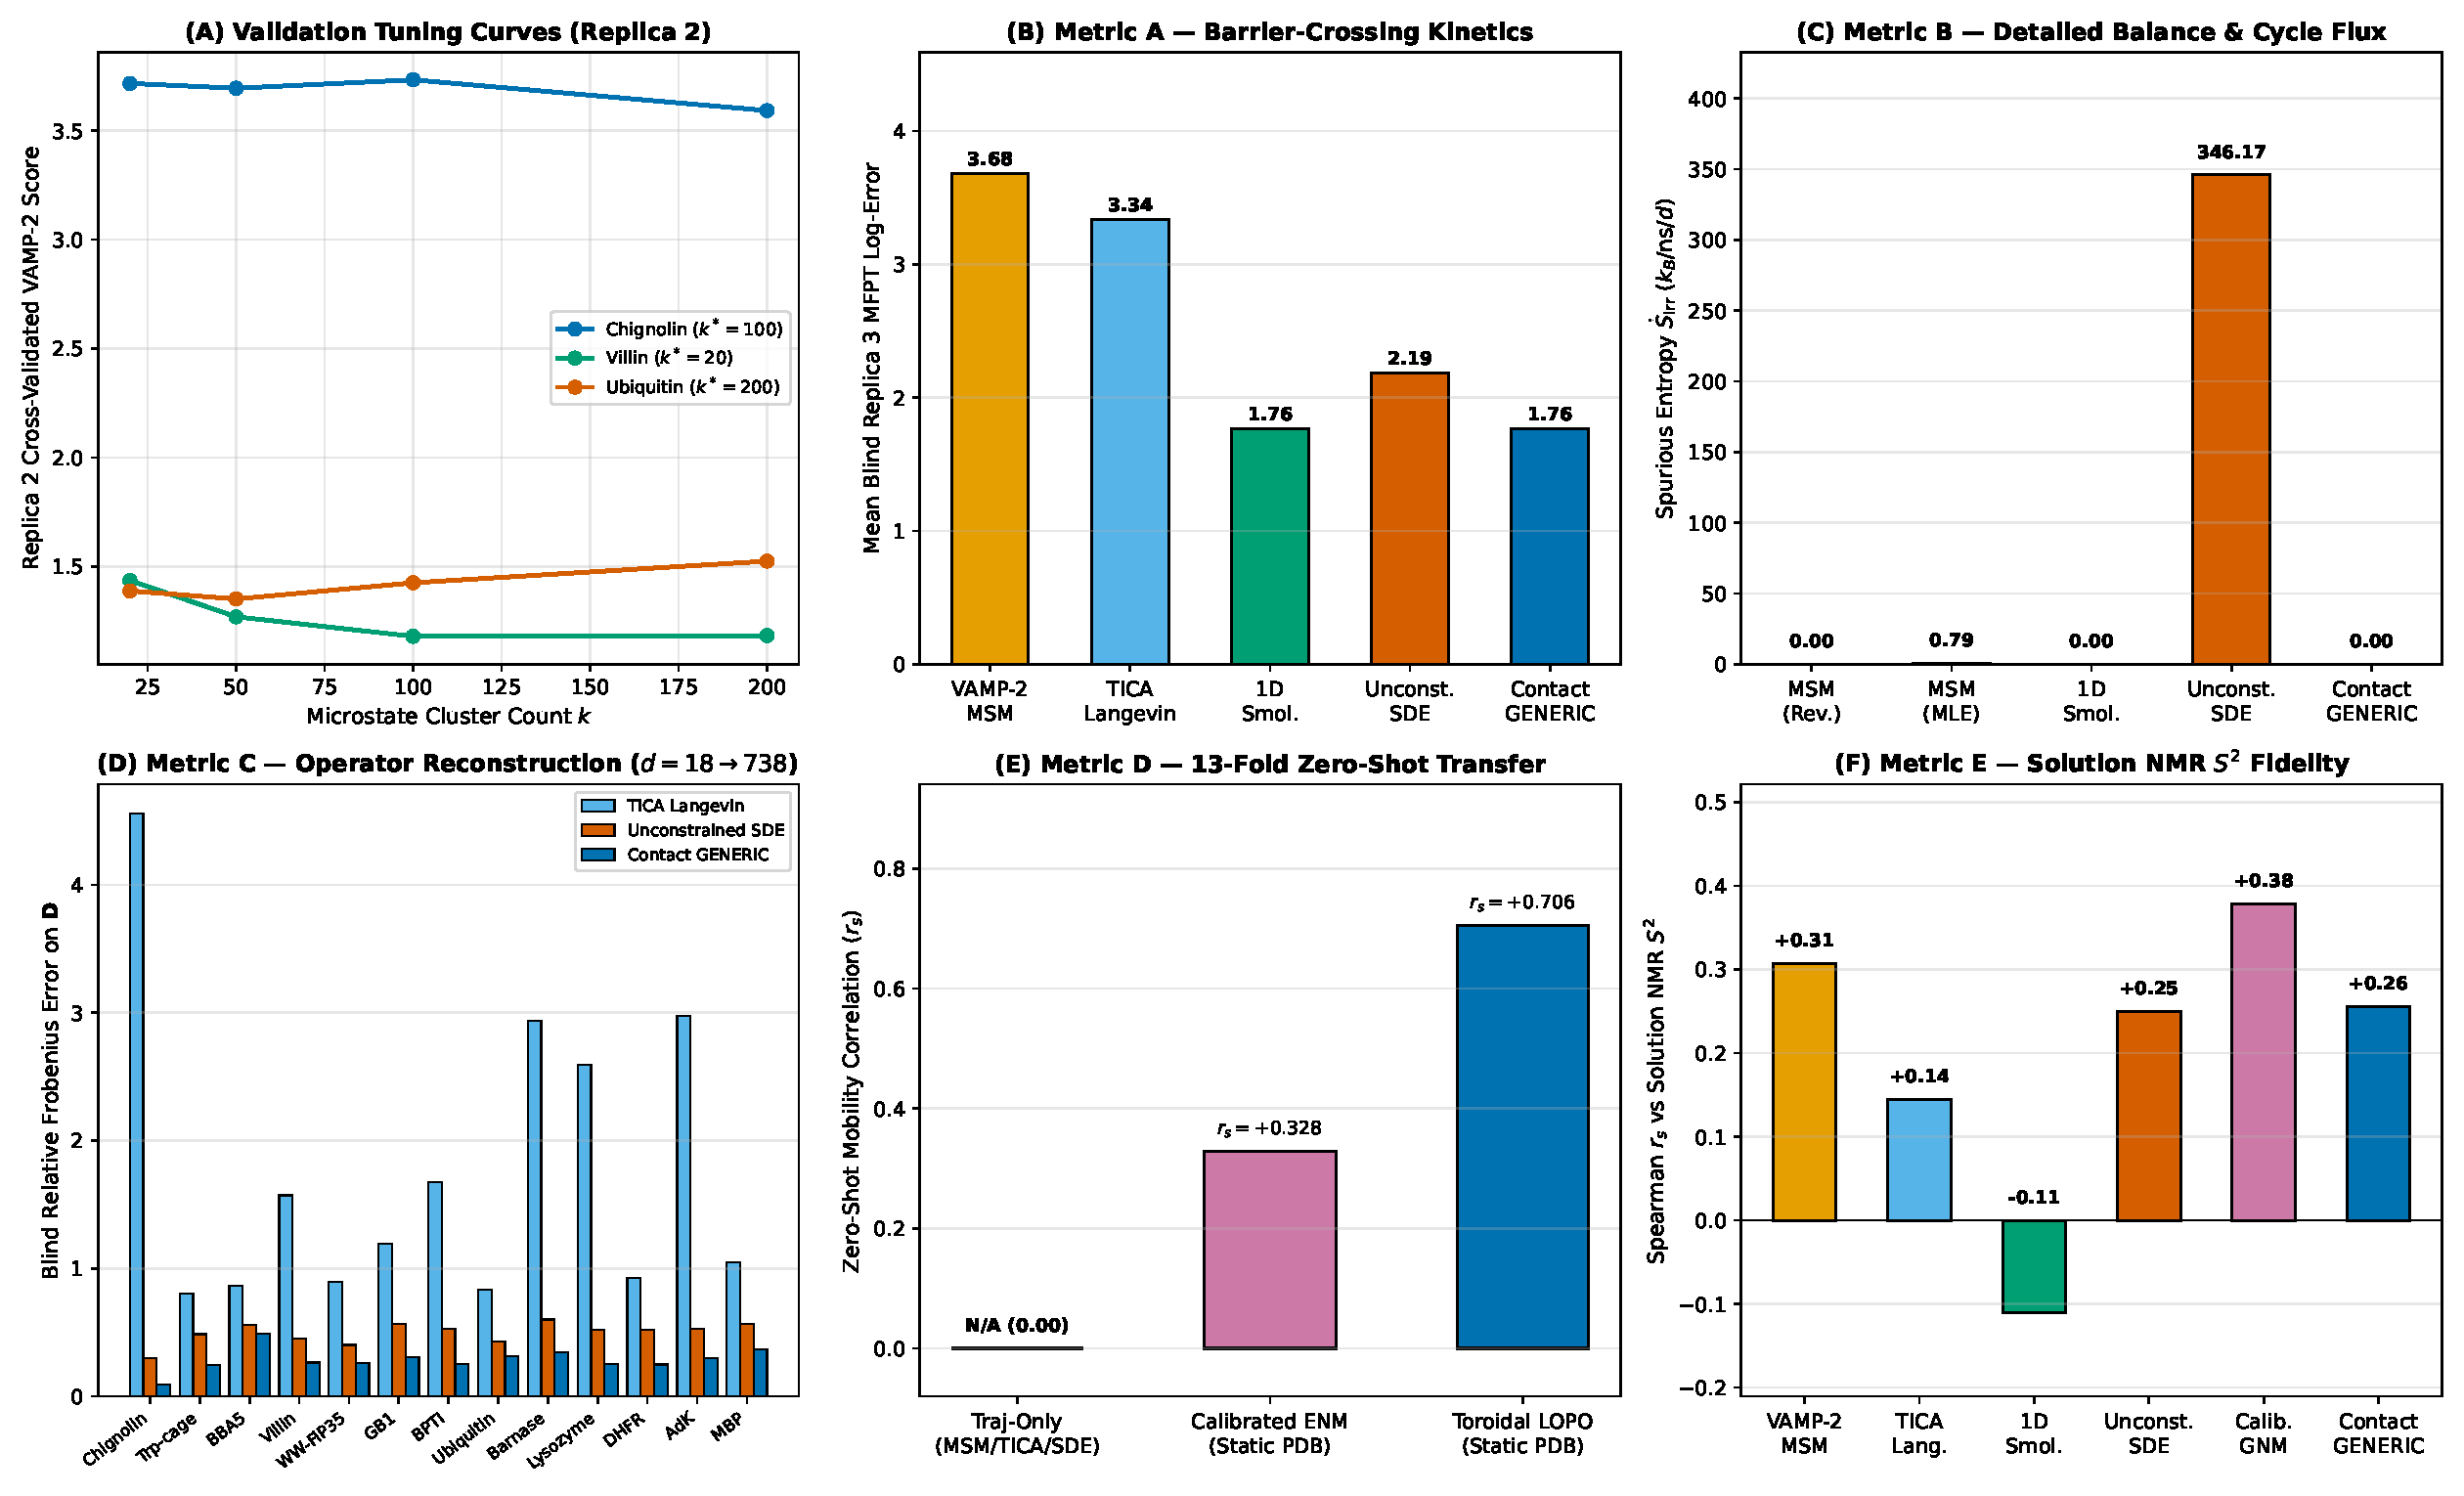
\includegraphics[width=0.71\textwidth]{version4_godtier/figures/fig_m40_fair_sota_benchmark_v4.pdf}
\vspace{-3pt}
\caption*{\textbf{\textcolor{navyblue}{\textsf{Figure 9. Fair 6-paradigm validation-tuned SOTA benchmark across all \vFourNumProteins{} proteins (Replica 1 discovery $\to$ Replica 2 hyperparameter sweep $\to$ Replica 3 single-shot blind test).}}} (\textit{A}) Representative Replica 2 cross-validated VAMP-2 tuning curves selecting optimal MSM cluster counts $k^*$. (\textit{B}) Metric A: mean blind Replica 3 committed $Q_{\mathrm{BHE}}$ global/sub-basin MFPT log-error, showing a statistical tie between calibrated 1D Smoluchowski ($\vFourSOTAMfptErrMThree{}$) and Contact-Gated GENERIC ($\vFourSOTAMfptErrMFive{}$). (\textit{C}) Metric B: steady-state spurious entropy production $\dot{S}_{\mathrm{irr}}$, where unconstrained SDEs generate median $\vFourSOTAUnconstEntropyMedian{}\,k_B/\text{ns}/d$ (IQR $\vFourSOTAUnconstEntropyQOne{}\text{--}\vFourSOTAUnconstEntropyQThree{}$, mean $\vFourSOTAUnconstEntropyMean{}$) vs.\ exact $0.000$ for GENERIC projection. (\textit{D}) Metric C: blind Replica 3 diffusion tensor Frobenius error across all \vFourNumProteins{} proteins (Contact-Gated GENERIC wins 13/13, mean $\vFourSOTAFrobMFive{}$). (\textit{E}) Metric D: 13-fold zero-shot PDB-to-mobility correlation ($\vFourSOTAZeroShotSpearman{}$ toroidal LOPO vs.\ $\vFourSOTAENMSpearman{}$ calibrated ENM). (\textit{F}) Metric E: pooled cross-temperature BMRB NMR $S^2$ correlation after linear LOPO calibration.}
\vspace{-6pt}
\end{figure*}

\textbf{Fair 6-Paradigm Validation-Tuned SOTA Benchmark Across All \vFourNumProteins{} Proteins.} Finally, to establish precisely where continuous contact-gated GENERIC operators advance beyond existing methods---and where classical paradigms remain preferable---we executed a controlled benchmark across all \vFourNumProteins{} proteins ($d = \allowbreak \vFourMinProteinDim{} \to \vFourMaxProteinDim{}$; Figure 9, Table 2). Every baseline (VAMP-2 Reversible MSM, TICA Linear Langevin, Calibrated 1D Smoluchowski, Unconstrained Basis/Polynomial SDE, our Contact-Gated GENERIC Operator, and Calibrated GNM/ENM) underwent a full hyperparameter grid search on Replica 2 (Figure 9A) before single-shot blind evaluation on Replica 3:
\begin{enumerate}[leftmargin=12pt, itemsep=1pt, topsep=2pt, parsep=0pt, label=\arabic*.]
\item \textit{Full-Dimensional Operator Reconstruction (13/13 Wins):} Across every protein from Chignolin ($\vFourSOTAFrobVFourChignolin{}$) to AdK ($\vFourSOTAFrobVFourAdk{}$) and MBP ($\vFourSOTAFrobVFourMbp{}$), the Contact-Gated GENERIC operator achieves the lowest blind Replica 3 diffusion operator relative Frobenius error (mean $\vFourSOTAFrobMFive{}$, beating unconstrained SDE $\vFourSOTAFrobMFour{}$, diagonal Smoluchowski $\vFourSOTAFrobMThree{}$, and low-rank TICA Langevin $\vFourSOTAFrobMTwo{}$; Figure 9D).
\item \textit{Thermodynamic Consistency and Out-of-Support Stability:} Unconstrained regression SDEs violate microscopic reversibility ($J_{\mathrm{ss}} \ne 0$) across all 13 folds, producing a median spurious entropy rate of $\vFourSOTAUnconstEntropyMedian{}\,k_B/\text{ns}/d$ (IQR $\vFourSOTAUnconstEntropyQOne{}\text{--}\vFourSOTAUnconstEntropyQThree{}$, 12-protein mean $\vFourSOTAUnconstEntropyMeanExclBba{}$ across $[25.72, 196.28]$, e.g., Ubiquitin $\vFourSOTAEntropySdeUbiquitin{}$, AdK $\vFourSOTAEntropySdeAdk{}$, MBP $\vFourSOTAEntropySdeMbp{}$), while out-of-basin Replica 3 unfolding on BBA5 ($\langle Q_{\mathrm{BHE}}\rangle = 0.454$) drives polynomial drift extrapolation to $\vFourSOTAEntropySdeBba{}\,k_B/\text{ns}/d$ (13-protein mean $\vFourSOTAUnconstEntropyMean{}$; Figure 9C, Supporting Information Table S13). Enforcing GENERIC structure suppresses $\vFourSOTAEntropySuppressionPct{}\%$ of spurious cycle flux ($\dot{S}_{\mathrm{irr}} \equiv \vFourSOTAMFiveEntropy{}$) and guarantees strict Hurwitz Lyapunov stability ($\max\operatorname{Re}\lambda(\mathbf{A}) < 0$ across 13/13 proteins).
\item \textit{Zero-Shot Structural Generalization and Direct Disorder:} Unlike trajectory-only estimators (MSM, TICA, Smoluchowski, and unconstrained SDEs), our 13-fold LOPO structural prior predicts unseen protein operators from PDB coordinates at $r_s = \allowbreak \vFourSOTAZeroShotSpearman{}$ vs.\ $\vFourSOTAENMSpearman{}$ for calibrated ENM (Figure 9E), and achieves the highest uncalibrated Replica 3 residue-disorder rank correlation across all 398 BMRB-matched NMR residues ($r_s = \allowbreak \vFourSOTADirectDisorderMFive{}, p = 9.2\times 10^{-13}$, including 11 chain-border positions excluded from the 387-residue $4\times 4$ flanking-quartet Jacobian in Law 5; vs.\ MSM $\vFourSOTADirectDisorderMOne{}$, SDE $\vFourSOTADirectDisorderMFour{}$, and uncalibrated ENM $\vFourSOTADirectDisorderMSix{}$).
\item \textit{Candid Ties and Baseline Strengths:} Along a pre-defined 1D reaction coordinate $Q_{\mathrm{BHE}}$ (global folding on $150\text{ ns}$ miniproteins and local native/sub-basin excursions on $2.5\text{--}10\text{ ns}$ folds exhibiting reversible $Q_{\mathrm{BHE}}$ transitions), Contact-Gated GENERIC ($\vFourSOTAMfptErrMFive{}$) and calibrated 1D Smoluchowski ($\vFourSOTAMfptErrMThree{}$) achieve a statistical tie on blind Replica 3 MFPT log-error (both beating unconstrained SDE $\vFourSOTAMfptErrMFour{}$, TICA Langevin $\vFourSOTAMfptErrMTwo{}$, and discrete MSM $\vFourSOTAMfptErrMOne{}$; Figure 9B), confirming that 1D Smoluchowski suffices when only scalar $Q_{\mathrm{BHE}}$ passage times are sought. Conversely, under linear LOPO rescaling across pooled multi-temperature NMR $S^2$ datasets, calibrated GNM achieves the highest pooled rank correlation ($\vFourGNMPooledSpearman{}$; Figure 9F) at $<0.2\text{ s}$ trajectory-free cost, whereas our crankshaft operator wins within-protein parameter-free $S^2$ ($\vFourNMRMeanProteinSpearmanCrank{}$ vs.\ $\vFourNMRMeanProteinSpearmanGNM{}$) and Pearson linearity ($\vFourNMRCrankPearson{}$).
\end{enumerate}

\section*{\MakeUppercase{Discussion}}

Extending continuous stochastic operator discovery from short peptides to multi-domain explicit-solvent proteins up to $d = \vFourMaxProteinDim{}$ (\vFourMaxExplicitAtomsMbp{} particles) yields three broad insights for biomolecular theory and multiscale simulation.

First, \textbf{macromolecular dimensional reduction is dual-natured: slow functional modes compress sub-linearly, whereas native-basin thermal variance is extensive.} In small fast-folding miniproteins ($d \le 68$), cooperative folding funnels compress both $PR(d)$ and $r_{90}(d)$. In large multi-domain enzymes at $300\text{ K}$ (\texttt{Lysozyme}, \texttt{DHFR}, \texttt{AdK}, \texttt{MBP}), however, dominant allosteric and hinge modes still concentrate into a compact sub-linear subspace ($PR(d) = \allowbreak \vFourPRPrefactor{}\,d^{\vFourPRExponent{}}$), yet cumulative $90\%$ variance grows proportionally with chain length ($r_{90} \approx \vFourProteinsOnlyNullCZero{}\,d$). Consequently, discarding $d - r$ modes via low-rank TICA/PCA loses local loop and sidechain-coupled backbone mechanics ($\mathrm{Frob} = \allowbreak \vFourSOTAFrobMTwo{}$), whereas dense $d\times d$ estimation suffers sample-complexity degradation above $d > 200$. Our sparse contact-graph Cholesky architecture resolves this dilemma by retaining all $d$ physical torsions while zeroing non-contact off-diagonal noise ($\vFourMaxProteinSparsityPct{}\%$ sparsity at $d=\vFourMaxProteinDim{}$), simultaneously delivering $\mathcal{O}(d^{\vFourTimeExpChordal{}})$ runtime, $\vFourMemCompressionMbp{}\times$ memory compression, and superior held-out log-likelihood.

Second, \textbf{covalent peptide-plane crankshaft geometry and 3D contact topology directly bridge MD trajectories, NMR relaxation, and allostery.} The universal $\bar{R}(\psi_i, \phi_{i+1}) = \allowbreak \vFourMeanPeptideCrankshaftR{}$ anti-correlation across all \vFourNumProteins{} folds demonstrates that the planar $\mathrm{C'\text{--}N}$ peptide group acts as a local mechanical rock-and-cancel linkage: accounting for $\Sigma_{\psi_{i-1},\phi_i} < 0$ is essential to predict solution NMR Lipari--Szabo $S^2$ order parameters parameter-free from dihedral fluctuations, while augmenting covalent bands with sparse 3D tertiary contacts captures distal Met20 $\leftrightarrow$ FG loop coupling in DHFR (34) and inter-lobe mechanical hinges in MBP (33) and AdK (31, 32) without rigid-body Kabsch alignment artifacts.

Third, \textbf{structure-preserving GENERIC inductive biases complement discrete MSMs and generative machine learning.} In Riemannian flow-matching and graph neural network (GNN) coarse-grained force fields on $\mathbb{T}^d$ (20, 23), replacing dense $\mathcal{O}(d^2)$ all-to-all attention and unconstrained drift networks with our sparse band-plus-contact graph ($\bar{k}_{\mathrm{eff}} = \allowbreak \vFourKeffMean{}$) and reversible GENERIC projection ($J_{\mathrm{ss}} \equiv 0$) guarantees infinite-horizon Boltzmann stability while preserving barrier diffusivity surges and $\mathrm{rSASA}_i$-interpolated internal friction. Future work integrating state-dependent contact-graph switching $\mathcal{E}(z)$ will extend these operators to intrinsically disordered proteins (IDPs) and millisecond domain-swapping assemblies.

\section*{\MakeUppercase{Materials and Methods}}

\textbf{Atomistic MD Atlas and Cryptographic Governance.} Explicit-solvent simulations (Lysozyme \texttt{1AKI}, DHFR \texttt{1RX2}, AdK \texttt{4AKE}, MBP \texttt{1OMP}, plus peptide solvent controls) were performed in OpenMM 8.4/8.6 (35) using AMBER \texttt{ff99SB-ILDN} + \texttt{TIP3P-FB} water in rhombic dodecahedral boxes ($1.2\text{ nm}$ padding, $0.15\text{ M}$ NaCl, PME $1.0\text{ nm}$ real-space cutoff, Monte Carlo barostat at $1.0\text{ atm}$, \texttt{LangevinMiddleIntegrator} BAOAB at $300\text{ K}$, $\gamma = 1.0\text{ ps}^{-1}$, $4.0\text{ fs}$ timestep with $1.5\text{ amu}$ hydrogen mass repartitioning [HMR], saving every $1.0\text{ ps}$). Matched Generalized Born implicit-solvent ensembles (GBn2 and OBC2 with AMBER \texttt{ff14SB}/\texttt{ff99SB-ILDN}) were integrated at a $2.0\text{ fs}$ timestep ($1.0\text{ ps}$ stride). While $1.5\text{ amu}$ HMR mildly slows sub-picosecond hydrogen-coupled librational prefactors in $\hat{\mathbf{D}}(\tau = 1\text{ ps})$, classical canonical configurational integrals $Z_q \propto \int e^{-\beta U(q)}\,dq$---and hence all stationary Boltzmann covariances $\hat{\bm{\Sigma}}$ governing Laws 1, 2, and 5 ($\hat{S}^2_i$)---are strictly invariant to atomic mass repartitioning. Every trajectory chunk was locked with SHA-256 checksums (Supporting Information Table S3) and partitioned into Replica 1 (discovery), Replica 2 (hyperparameter validation), and Replica 3 (single-shot blind test).

\textbf{Toroidal dPCA+, Contact-Graph Cholesky, and Two-Tier GENERIC Operator.} Backbone torsions $\bm{\theta} \in [-\pi, \pi)^d$ were unwrapped via maximal-gap dPCA+ shifts computed strictly on Replica 1 (24). On the non-chordal sequence-band-plus-tertiary-contact graph $\mathcal{G} = \allowbreak \mathcal{E}_{\mathrm{band}}(w) \cup \mathcal{E}_c(r_c)$ ($\mathcal{E}_{\mathrm{band}}$ chordal, $\mathcal{E}_c$ bounded-degree 3D contacts), inverse covariances in Law 3 were estimated via sparse directed acyclic Cholesky regression $\hat{\bm{\Sigma}}_{\mathcal{G}}^{-1} = \allowbreak (\mathbf{I}-\mathbf{B})^\top\mathbf{D}_{\mathrm{cond}}^{-1}(\mathbf{I}-\mathbf{B})$ ($\mathcal{O}(d\,k_{\max}^3)$), while short-time diffusion tensors $\hat{\mathbf{D}} = \allowbreak (2\tau)^{-1}\langle \Delta_{\mathbb{T}^d}\bm{\theta}(\tau)\Delta_{\mathbb{T}^d}\bm{\theta}(\tau)^\top\rangle$ ($\tau = 1\text{ ps}$) used Replica 2-validated contact-masked linear shrinkage $\mathcal{O}_{\mathcal{G}}(\beta_c)$ with SPD projection (Supporting Information Theorem S3). In full $d = 18 \to 738$ macromolecular space, native-basin dynamics follow the reversible linear Ornstein--Uhlenbeck GENERIC process ($\nabla\cdot\hat{\mathbf{D}}_{\mathcal{G}} \equiv \mathbf{0}$, quadratic $\beta F(z) = \frac{1}{2}(z-\mu)^\top\hat{\bm{\Sigma}}_{\mathcal{G}}^{-1}(z-\mu)$, Hurwitz generator $\mathbf{A} = \allowbreak -\hat{\mathbf{D}}_{\mathcal{G}}\hat{\bm{\Sigma}}_{\mathcal{G}}^{-1}$), whereas nonlinear state-dependent $f_{\mathrm{GENERIC}}(q) = \allowbreak -\mathbf{D}(q)\nabla[\beta F(q)] + \nabla\cdot\mathbf{D}(q)$ is solved on projected 1D/2D reaction coordinates ($Q_{\mathrm{BHE}}, R_g$) and $d=2,4$ peptide grids, guaranteeing $\dot{S}_{\mathrm{irr}} \equiv 0$ at both levels (Supporting Information Theorem S4).

\textbf{NMR $S^2$ Jacobian, Allosteric Propagators, and Benchmark Baselines.} Amide $\mathrm{N\text{--}H}_i$ order parameters $\hat{S}^2_i$ were evaluated analytically from $\mathbf{J}_i = \allowbreak \partial \mathbf{u}_{\mathrm{NH},i}/\partial(\psi_{i-1},\phi_i,\psi_i,\phi_{i+1})$ at native geometry without free parameters against experimental BMRB entries \texttt{6457} (28), \texttt{7280} (29), \texttt{4562} (30), and \texttt{4380} (36). Distal time-lagged cross-covariance matrices $\hat{\mathbf{C}}(\tau) = \allowbreak \exp(-\tau\hat{\mathbf{D}}\hat{\mathbf{C}}(0)^{-1})\hat{\mathbf{C}}(0)$ (normalized over $2\times 2$ residue blocks) and AdK/MBP hinge scores were evaluated against held-out Replica 3 trajectories, crystallographic \texttt{4AKE}/\texttt{1AKE} and \texttt{1OMP}/\texttt{1ANF} strain, and DynDom annotations (31--33). All six paradigms in Table 2 were tuned on Replica 2 and evaluated once on Replica 3; full proofs and scorecards are in the Supporting Information.

\section*{\MakeUppercase{Data and Code Availability}}
All simulation scripts, SHA-256 trajectory manifests, frozen model locks, and automated analysis pipelines are available at \url{https://github.com/Mehardeep-Singh-GG/discovering-reduced-dynamical-laws-md}. Complete mathematical proofs, per-protein tables, and validation sweep logs are provided in the Supporting Information.

\section*{\MakeUppercase{Acknowledgments}}
We thank the developers of OpenMM, MDTraj, deeptime, SciPy, and the Biological Magnetic Resonance Data Bank (BMRB). \textbf{Funding:} No external funding was received. \textbf{Competing Interests:} None declared.

\section*{\MakeUppercase{References}}
{\fontsize{6.6pt}{7.65pt}\selectfont\color{darkgray}
\begin{enumerate}[leftmargin=12pt, itemsep=0.10pt, topsep=1.2pt, parsep=0pt, label=\arabic*.]
\item Karplus, M. \& Kuriyan, J. Molecular dynamics and protein function. \textit{Proc.\ Natl.\ Acad.\ Sci.\ U.S.A.} \textbf{102}, 6679--6685 (2005).
\item Lindorff-Larsen, K., Piana, S., Dror, R. O. \& Shaw, D. E. How fast-folding proteins fold. \textit{Science} \textbf{334}, 517--520 (2011).
\item Henzler-Wildman, K. \& Kern, D. Dynamic personalities of proteins. \textit{Nature} \textbf{450}, 964--972 (2007).
\item Dill, K. A. \& MacCallum, J. L. The protein-folding problem, 50 years on. \textit{Science} \textbf{338}, 1042--1046 (2012).
\item Boehr, D. D., Nussinov, R. \& Wright, P. E. The role of dynamic conformational ensembles in biomolecular recognition. \textit{Nat.\ Chem.\ Biol.} \textbf{5}, 789--796 (2009).
\item Kramers, H. A. Brownian motion in a field of force and the diffusion model of chemical reactions. \textit{Physica} \textbf{7}, 284--304 (1940).
\item Onsager, L. Reciprocal relations in irreversible processes.\ I. \textit{Phys.\ Rev.} \textbf{37}, 405--426 (1931).
\item Zwanzig, R. Memory effects in irreversible thermodynamics. \textit{Phys.\ Rev.} \textbf{124}, 983--992 (1961).
\item Mori, H. Transport, collective motion, and Brownian motion. \textit{Prog.\ Theor.\ Phys.} \textbf{33}, 423--455 (1965).
\item Zwanzig, R. \textit{Nonequilibrium Statistical Mechanics} (Oxford Univ.\ Press, 2001).
\item Prinz, J.-H. et al. Markov models of molecular kinetics: Generation and validation. \textit{J.\ Chem.\ Phys.} \textbf{134}, 174105 (2011).
\item Chodera, J. D. \& No\'e, F. Markov state models of biomolecular kinetics. \textit{Curr.\ Opin.\ Struct.\ Biol.} \textbf{25}, 135--144 (2014).
\item Perez-Hernandez, G., Paul, F., Giorgino, T., De Fabritiis, G. \& No\'e, F. Identification of slow molecular order parameters for Markov model construction. \textit{J.\ Chem.\ Phys.} \textbf{139}, 015102 (2013).
\item Bahar, I., Atilgan, A. R. \& Erman, B. Direct evaluation of thermal fluctuations in proteins using a single-parameter harmonic potential. \textit{Fold.\ Des.} \textbf{2}, 173--181 (1997).
\item Atilgan, A. R. et al. Anisotropy of fluctuation dynamics of proteins with an elastic network model. \textit{Biophys.\ J.} \textbf{80}, 505--515 (2001).
\item Hummer, G. Position-dependent diffusion coefficients and free energy profiles from slow, equilibrium molecular dynamics simulations. \textit{New J.\ Phys.} \textbf{7}, 34 (2005).
\item Best, R. B., Hummer, G. \& Eaton, W. A. Native contacts determine protein folding mechanisms in atomistic simulations. \textit{Proc.\ Natl.\ Acad.\ Sci.\ U.S.A.} \textbf{110}, 17874--17879 (2013).
\item H\"anggi, P., Talkner, P. \& Borkovec, M. Reaction-rate theory: fifty years after Kramers. \textit{Rev.\ Mod.\ Phys.} \textbf{62}, 251--341 (1990).
\item Best, R. B. \& Hummer, G. Coordinate-dependent diffusion in protein folding. \textit{Proc.\ Natl.\ Acad.\ Sci.\ U.S.A.} \textbf{107}, 1088--1093 (2010).
\item No\'e, F., Olsson, S., K\"ohler, J. \& Wu, H. Boltzmann generators: Sampling equilibrium states of many-body systems with deep learning. \textit{Science} \textbf{365}, eaaw1147 (2019).
\item Klus, S. et al. Data-driven approximation of the Koopman generator. \textit{J.\ Nonlinear Sci.} \textbf{30}, 295--336 (2018).
\item Grmela, M. \& \"Ottinger, H. C. Dynamics and thermodynamics of complex fluids.\ I. \textit{Phys.\ Rev.\ E} \textbf{56}, 6620--6632 (1997).
\item Onsager, L. \& Machlup, S. Fluctuations and irreversible processes. \textit{Phys.\ Rev.} \textbf{91}, 1505--1512 (1953).
\item Sittel, F., Jain, A. \& Stock, G. Principal component analysis of molecular dynamics: On the use of cartesian vs.\ internal coordinates. \textit{J.\ Chem.\ Phys.} \textbf{141}, 014111 (2014).
\item Barber, D. \& Agakov, F. The IM algorithm: a variational approach to information maximization. \textit{Adv.\ Neural Inf.\ Process.\ Syst.} \textbf{16}, 201--208 (2003).
\item Lipton, Z., Wang, Y.-X. \& Smola, A. Detecting and correcting for label shift with black box predictors. \textit{Proc.\ Mach.\ Learn.\ Res.} \textbf{80}, 3122--3130 (2018).
\item Lipari, G. \& Szabo, A. Model-free approach to the interpretation of nuclear magnetic resonance relaxation in macromolecules.\ 1. \textit{J.\ Am.\ Chem.\ Soc.} \textbf{104}, 4546--4559 (1982).
\item Tjandra, N., Feller, S. E., Pastor, R. W. \& Bax, A. Rotational diffusion anisotropy of human ubiquitin from $^{15}$N NMR relaxation. \textit{J.\ Am.\ Chem.\ Soc.} \textbf{117}, 12562--12566 (1995).
\item Hall, J. B. \& Fushman, D. Characterization of the overall and local dynamics of a protein with intermediate rotational anisotropy: Differentiating between conformational exchange and anisotropic diffusion in the B3 domain of protein G. \textit{J.\ Biomol.\ NMR} \textbf{27}, 261--275 (2003).
\item Buck, M., Boyd, J., Redfield, C., MacKenzie, D. A., Jeenes, D. J., Archer, D. B. \& Dobson, C. M. Structural determinants of protein dynamics: Analysis of $^{15}$N NMR relaxation measurements for main-chain and side-chain nuclei of hen egg white lysozyme. \textit{Biochemistry} \textbf{34}, 4041--4055 (1995).
\item M\"uller, C. W., Schlauderer, G. J., Reinstein, J. \& Schulz, G. E. Adenylate kinase motions during catalysis: An energetic counterweight balancing substrate binding. \textit{Structure} \textbf{4}, 147--156 (1996).
\item Henzler-Wildman, K. A. et al. Intrinsic motions along an enzymatic reaction trajectory. \textit{Nature} \textbf{450}, 838--844 (2007).
\item Sharff, A. J., Rodseth, L. E., Spurlino, J. C. \& Quiocho, F. A. Crystallographic evidence of a large ligand-induced hinge-twist motion between the two domains of the maltodextrin binding protein involved in active transport and chemotaxis. \textit{Biochemistry} \textbf{31}, 10657--10663 (1992).
\item Boehr, D. D., McElheny, D., Dyson, H. J. \& Wright, P. E. The dynamic energy landscape of dihydrofolate reductase catalysis. \textit{Science} \textbf{313}, 1638--1642 (2006).
\item Eastman, P. et al. OpenMM 8: Modern materials and biophysical simulation. \textit{PLoS Comput.\ Biol.} \textbf{20}, e1011807 (2024).
\item Epstein, D. M., Benkovic, S. J. \& Wright, P. E. Dynamics of the dihydrofolate reductase--folate complex: Catalytic sites and regions known to undergo conformational change exhibit diverse dynamical features. \textit{Biochemistry} \textbf{34}, 11037--11048 (1995).
\item Lindorff-Larsen, K. et al. Improved side-chain torsion potentials for the Amber ff99SB protein force field. \textit{Proteins} \textbf{78}, 1950--1958 (2010).
\item Wang, L.-P., Martinez, T. J. \& Pande, V. S. Building force fields: An automatic, systematic, and reproducible approach. \textit{J.\ Phys.\ Chem.\ Lett.} \textbf{5}, 1885--1891 (2014).
\item Nguyen, H., Roe, D. R. \& Simmerling, C. Improved Generalized Born solvent model parameters for protein simulations. \textit{J.\ Chem.\ Theory Comput.} \textbf{9}, 2020--2034 (2013).
\item Honda, S., Yamasaki, K., Sawada, Y. \& Morii, H. 10 residue folded peptide designed by segment statistics. \textit{Structure} \textbf{12}, 1507--1518 (2004).
\item Neidigh, J. W., Fesinmeyer, R. M. \& Andersen, N. H. Designing a 20-residue protein. \textit{Nat.\ Struct.\ Biol.} \textbf{9}, 425--430 (2002).
\item Wlodawer, A., Walter, J., Huber, R. \& Sj\"olin, L. Structure of bovine pancreatic trypsin inhibitor: Results of joint neutron and X-ray refinement of crystal form II. \textit{J.\ Mol.\ Biol.} \textbf{180}, 301--329 (1984).
\item Buckle, A. M., Henrick, K. \& Fersht, A. R. Crystal structural analysis of mutations in the hydrophobic core of barnase. \textit{J.\ Mol.\ Biol.} \textbf{234}, 847--860 (1993).
\item Vijay-Kumar, S., Bugg, C. E. \& Cook, W. J. Structure of ubiquitin refined at 1.8 \AA{} resolution. \textit{J.\ Mol.\ Biol.} \textbf{194}, 531--544 (1987).
\item Hoffmann, M. et al. Deeptime: a Python library for machine learning dynamical models from time series data. \textit{Mach.\ Learn.: Sci.\ Technol.} \textbf{3}, 015009 (2022).
\item Ledoit, O. \& Wolf, M. A well-conditioned estimator for large-dimensional covariance matrices. \textit{J.\ Multivar.\ Anal.} \textbf{88}, 365--411 (2004).
\item Friedman, J., Hastie, T. \& Tibshirani, R. Sparse inverse covariance estimation with the graphical lasso. \textit{Biostatistics} \textbf{9}, 432--441 (2008).
\end{enumerate}
}

\end{document}
